%This template was prepared by Dorothea F. Brosius of the 
%Institute for Electronics and Applied Physics, University of Maryland, College Park, MD
%The template was last updated in April 2012
%Thesis Main Page used with thesis.sty based on the
%University of Maryland Electronic Thesis and Dissertation (ETD) Style Guide

\documentclass[12pt]{thesis}  %12pt is larger than 11pt
%\usepackage[pctex32]{graphics}
\author{Jiabin Wang}
\title{Master Thesis of software engineering -- 2}
\usepackage{graphicx}
\usepackage{lscape}
\usepackage{indentfirst}
\usepackage{latexsym}
\usepackage{multirow}
\usepackage{tabls}
\usepackage{wrapfig}
\usepackage{amsmath}
\usepackage{slashbox}
\usepackage{longtable}
\usepackage{supertabular}
\usepackage{caption}
\usepackage{subcaption}
\usepackage[table]{xcolor}
\renewcommand{\baselinestretch}{2}
\setlength{\textwidth}{5.9in}
\setlength{\textheight}{9in}
\setlength{\topmargin}{-.50in}
%\setlength{\topmargin}{0in}    %use this setting if the printer makes the the top margin 1/2 inch instead of 1 inch
\setlength{\oddsidemargin}{.55in}
\setlength{\parindent}{.4in}
\pagestyle{empty}

\begin{document}
%Abstract Page 

\hbox{\ }

\renewcommand{\baselinestretch}{2}
\small \normalsize
\begin{center}
\textbf{Automated Classification of Massive Scale Image Data}
\end{center}
\begin{center}
by
\end{center}
\begin{center}
Jiabin Wang
\end{center}
\begin{center}
December 2016
\end{center}
Director of Thesis:  Dr. Junhua Ding\\
Major Department:  Computer Science\par

\large \normalsize

The diffraction image is a useful method to facilitate the representation of tiny entities such as the cell. It provides an efficient way to analyze the 3D morphological features of biological cells.   However, the representation of diffraction images is so abstract that classifying them is challenging. When it comes to the massive amount of diffraction images, a manual classification for them can be time-consuming, and their accuracy cannot be guaranteed. This research focuses on the automated classification of diffraction images with high accuracy. In this research, gray level co-occurrence matrix (GLCM) that is a Statistical method for image texture analysis is used to extract texture features and the support vector machine (SVM) algorithm is applied for classification among three types of diffraction image based on image texture features. These types are cell, debris, and strip. \par
Two diffraction images which are captured at the same time but from different directions are combined together to improve the pattern recognition of the diffraction image. The diffraction image is processed by a developed JAVA application into a numerical data example which contains 34 texture features. The application is implemented with simple User Interface (UI) to facilitate user's operation of the application. In contrast to two existing tools implemented in MATLAB and C++, the JAVA application provides a new functionality that allows users to modify the primary parameters of GLCM without changing the code. A case study is performed for selecting feature parameters. From the case study, 28 out of 34 texture features are selected as feature parameters applied for the SVM. Thus, a stable SVM classifier is attained using these feature parameters. Finally, an improvement process is performed by identifying the parameter pair of Radial Basis Function (RBF) kernel. Through assigning the parameter pair with ($C = 2^{12}$,$\gamma = 2^{-3}$), the classification accuracy is improved to 80.33\%. As the confusion matrix shows, the SVM classifier we selected from the experiment has high performance in selecting the cell and debris image types. Their accuracy is 88.76\% and 88.75\%.   
\newpage
\mbox{}
 %(must be first, required, non-numbered)
\newpage

%Pages from this point start at lower-case Roman number ii)
\pagestyle{plain}
\pagenumbering{roman}
\setcounter{page}{1}


%Titlepage

\thispagestyle{empty}
\hbox{\ }
\vspace{1in}
\renewcommand{\baselinestretch}{2}
\small\normalsize
\begin{center}

\textbf{Automated Classification of Massive Scale Image Data}

\vspace{2cm}

A Thesis\\
Presented To the Faculty of the Department of Computer Science\\
East Carolina University

\vspace{3cm}

In Partial Fulfillment of the Requirements for the Degree\\
Master of Science in Software Engineering

\vspace{3cm}

by\\
Jiabin Wang\\
December, 2016

\end{center}
 %(must follow Abstract, required, non-numbered)
%Copyright

\thispagestyle{empty}
\hbox{\ }

\vfill
\renewcommand{\baselinestretch}{1}
\small\normalsize

\vspace{-.65in}

\begin{center}
\large{\copyright \hbox{ }Jiabin Wang, 2016 }  %Type your name as it appears %in University records

\end{center}

\vfill
 %(highly recommended, non-numbered)

%Signature Page 

\hbox{\ }

\renewcommand{\baselinestretch}{2}
\small \normalsize
\begin{center}
\textbf{Automated Classification of Massive Scale Image Data}
\end{center}
\begin{center}
by
\end{center}
\begin{center}
Jiabin Wang
\end{center}
 
\begin{flushleft}
APPROVED BY:
\end{flushleft}
DIRECTOR OF\\ 
THESIS:
\noindent\rule{14cm}{0.4pt}
\begin{flushright}
\renewcommand{\baselinestretch}{0}
\small\normalsize
(Junhua Ding, PhD)
\end{flushright}
COMMITTEE MEMBER: 
\noindent\rule{10.75cm}{0.4pt}
\begin{flushright}
\renewcommand{\baselinestretch}{0}
\small\normalsize
(Type Name, Degree Here)
\end{flushright}
COMMITTEE MEMBER: 
\noindent\rule{10.75cm}{0.4pt}
\begin{flushright}
\renewcommand{\baselinestretch}{0}
\small\normalsize
(Type Name, Degree Here)
\end{flushright}
CHAIR OF THE DEPARTMENT\\ 
OF COMPUTER SCIENCE:
\noindent\rule{10.4cm}{0.4pt}
\begin{flushright}
\renewcommand{\baselinestretch}{0}
\small\normalsize
(Type Name, Degree Here)
\end{flushright}
DEAN OF THE\\ 
GRADUATE SCHOOL: 
\noindent\rule{11.3cm}{0.4pt}
\begin{flushright}
\renewcommand{\baselinestretch}{0}
\small\normalsize
(Paul J. Gemperline, PhD)
\end{flushright}
	

%Acknowledgments

\renewcommand{\baselinestretch}{2}
\small\normalsize
\hbox{\ }
\thispagestyle{empty} 
\vspace{-.65in}

\begin{center}
\large{ACKNOWLEDGEMENTS} 
\end{center} 

\vspace{1ex}

I would like to appreciate my supervisor Dr. Junhua Ding for his tireless guidance and funding. I would like to appreciate Dr. Xin-Hua Hu for providing me the background knowledge and all the diffraction images. I also would like to thank my committee members Dr. Tabrizi and Dr. Vilkomir for taking to time to attend my thesis defense and providing feedback. I am  grateful for having Dr. Hills, Dr. George Wang and all professors and students in my thesis defense. Finally, I want to thank Dr. Tedesco for reviewing my thesis and providing feedback on grammar.  


%\include{Preface}  %(if present, start at lower-case Roman number ii)
%\include{Foreword} %(if present, lower-case Roman)
%\include{Dedication} %(if present, lower-case Roman)
%%Acknowledgments

\renewcommand{\baselinestretch}{2}
\small\normalsize
\hbox{\ }
\thispagestyle{empty} 
\vspace{-.65in}

\begin{center}
\large{ACKNOWLEDGEMENTS} 
\end{center} 

\vspace{1ex}

I would like to appreciate my supervisor Dr. Junhua Ding for his tireless guidance and funding. I would like to appreciate Dr. Xin-Hua Hu for providing me the background knowledge and all the diffraction images. I also would like to thank my committee members Dr. Tabrizi and Dr. Vilkomir for taking to time to attend my thesis defense and providing feedback. I am  grateful for having Dr. Hills, Dr. George Wang and all professors and students in my thesis defense. Finally, I want to thank Dr. Tedesco for reviewing my thesis and providing feedback on grammar.  
 %(if present, lower-case Roman)

\renewcommand{\baselinestretch}{1}
\small\normalsize

\pagestyle{empty}{
	\renewcommand{\thispagestyle}[1]{}
    \tableofcontents %(required, lower-case Roman)
	\newpage
    \listoftables %(if present, lower-case Roman)
    \newpage
	\listoffigures %(if present, lower-case Roman)
}
\newpage

% LIST OF ABBREVIATIONS
\addcontentsline{toc}{chapter}{List of Abbreviations}
%List of Abbreviations

\renewcommand{\baselinestretch}{1}
\small\normalsize
\hbox{\ }

\vspace{-4em}

\begin{center}
\large{List of Abbreviations}
\end{center} 

\vspace{3pt}

\begin{tabular}{ll}
ASM & Angular Second Moment \\
API & Application Program Interface\\
\\
BUS & Breast Lesions on Ultrasound \\
\\
CON & Contrast \\
COR & Correlation \\
CLS & Cluster Shade \\
CLP & Cluster Prominence \\
CSV & Comma-Separated Values\\
\\
DEN & Difference Entropy \\
DVA & Difference Variance \\
DIS & Dissimilarity \\

\\
ENT & Entropy \\
\\
RBF & Radial Basis Function \\
\\
GLCM & Gray Level Co-occurrence Matrix\\
\\
IDM & Inverse Difference Moment \\
IMIN & Relative Minimum Pixel Intensity\\
IMAX & Relative Maximum Pixel Intensity\\
IMEA & Mean Value of Pixel Intensity\\
\\
MIP & Minimum Probability \\
MAP & Maximum Probability \\
MEA & Mean \\
\\
SVM & Support Vector Machine \\
SAR & Synthetic Aperture Radar\\
SAV & Sum Average \\
SEN & Sum Entropy \\
SVA & Sum Variance \\
\\
UI & User Interface \\
\\
VAR & Variance 
\end{tabular}



\setlength{\parskip}{0em}
\renewcommand{\baselinestretch}{2}
\small\normalsize

\newpage
%Pages from this point start at Arabic numeral 1
\pagestyle{plain}
\setcounter{page}{1}
\pagenumbering{arabic}

%Chapter 1

\renewcommand{\thechapter}{1}

\chapter{Introduction}

Big data is a term that describes the large amount or high complexity of data sets. With the rapid development of information technology, the concept of big data becomes more and more prevalent. Since the data sets are large or complex, traditional data processing applications are inadequate to handle them\cite{Snijders}. Image data is a direct representation of an entity or object using pictorial information and, because of that, is widely applied in many research fields such as biology, physics, geology, medicine and so on. The diffraction image is a kind of image data that makes tiny entities more visible to the observer. For instance, it provides an efficient way for analysis of three-dimensional (3D) morphological features of biological cells\cite{Brown}. However, the representation of diffraction images is so abstract that it is challenging for observers to classify them. When it comes to the concept of big data, manually processing them is time-consuming, and the accuracy which depends on the experience and skills of observers cannot be guaranteed. Based on the concept of digital imaging, image data can be represented by physical points called pixel\cite{Foley}. With the resolution of images enhanced, the analysis for images becomes tougher and tougher. Therefore, analyst involves texture analysis which is a common method that is widely used to analyze image texture that can provide the spatial relationship of intensities in an image or selected segment of an image\cite{Linda}. Within all the best methods of texture analysis, gray level co-occurrence matrix (GLCM) is the most useful approach because it is easy for the analyst to learn and be extensively applied\cite{Nanni}. To perform the method, GLCM is created by counting the spatial relation between two pixels over the whole image, and the texture of GLCM, such as contrast, correlation, energy, or homogeneity, is calculated from the GLCM. Machine learning is one of the state-of-the-art approaches to deal with analyzing the massive amount of data. Practically speaking, machine learning is the process that provides the computer the ability to grow and improve by itself with certain data sets\cite{Mitchell}. It constructs an algorithm that enables the computer to learn from and predict data\cite{Mehryar}. By applying the concept of machine learning, the computer is enabled to process a massive amount of specific data with the corresponding model. However, to achieve the model used in machine learning requires certain data to train. Support vector machine (SVM) algorithm is a kind of supervised learning model in machine learning to facilitate classification, regression, or other tasks\cite{Cortes}. In SVM algorithm, given a set of labeled data, the SVM algorithm can build a classifier to predict new unlabeled data. In general, the training data in a vector contains multiple feature parameters. For instance, a tumor diagnosis model is trained on a certain amount of data that contains patient's age and the tumor's size, as well as the corresponding label which is either benign or malignant. By providing the unknown data with the same format, the model is able to label the example either benign or malignant. To validate whether the SVM algorithm can be applied for image classification based on texture features extracted from GLCM, a case study was conducted. Finally, kernel methods are widely applied in SVM, which enables SVM to be competitive with neural networks on some tasks such as handwriting recognition\cite{Aizerman}.   \par 
This thesis research focuses on applying the SVM algorithm for classification based on texture features of diffraction images. First, we want to develop and verify a GLCM calculation tool for extracting texture features because the existing tools cannot be satisfied with the requirements. Then, we want to validate whether the SVM algorithm can be applied for classification by using texture features of the diffraction image. Finally, we want to validate whether the parameters of kernel methods affect the performance of the SVM classifier. \par
Through this thesis study, we have developed a GLCM application for extracting texture features from diffraction images. In contrast to two existing tools implemented in MATLAB and C++, the newly developed application provides simple User Interface (UI) for users. Thus, users who do not have programming skills can modify the parameter offset and parameter angle direction without changing the code when creating the GLCM. Furthermore, we have verified the newly developed application through functionality testing. Based on the results of testing, we have debugged some defects in the component which is used to load the image data and convert image data to a numerical pixel matrix. We also have verified that the difference between tools implemented in MATLAB and JAVA is caused by the way the applications realize the texture features from GLCM. In the JAVA application, we implemented the common algorithms which are defined by Haralick for calculating texture features\cite{Haralick}. We also have validated that the SVM can be applied for classification based on the texture feature of the diffraction image. Instead of using an extensive feature correlation study and fully automated algorithm CFS for selecting feature parameters, the validation process has fully utilized the tool LIBSVM to select feature parameters and examine how each texture feature or texture feature combination affects the classification accuracy of SVM. In addition, we have selected the SVM classifier with the highest accuracy by modifying the parameters of radial basis function (RBF) kernel. Finally, we have proved that the representation of diffraction images can be improved by using two diffraction images which are captured at the same time but from different directions. \par
This thesis is organized into the following chapters. Chapter 2 mainly presents the GLCM. In this chapter, we present a detailed description of GLCM. Following the description, the thesis demonstrates the development of GLCM texture feature calculation application in JAVA and a procedure to verify all the applications. In the end of chapter 2, we draw a brief conclusion. Chapter 3 provides the procedure for selecting an SVM classifier. This chapter, it starts with experiment data preprocessing. Then, it describes the experiment method we proposed step by step with the results of each step. It also discusses the validation of the SVM classifier, and we propose another method for selecting the SVM classifier to mitigate the limitations of the first approach. This chapter also presents the SVM kernel and the parameter pair of the RBF kernel, and we demonstrate the modification process to achieve the highest accuracy of the classifier. Finally, chapter 4 provides a summary of the whole thesis.      
%Chapter 2

\renewcommand{\thechapter}{2}

\chapter{Image Texture Analysis}

\section{Texture Analysis Using GLCM Algorithm}

\subsection{Overview}
Grey-Level Co-occurrence Matrix (GLCM) is a common method to represent the distance and angular spatial relationship over the image with a whole segment or sub-segment of specific size. It is created from the array of pixels of an image. Texture is a term to describe an image in another way. The texture measurements of GLCM is firstly proposed by Haralick in the 1970s for image classification\cite{Haralick}. And then, it is widely applied into many fields to solve some specific problems such as the classification of breast lesions on ultrasound (BUS) images\cite{Gomez} and the analysis for synthetic aperture radar (SAR) imagery\cite{Umasankar}. In general, GLCM is a statistic method for calculating the frequency between the pixel of reference and its neighbor. It is created by counting the total number of pairs occurred in the array of pixels. Each pair consists of the reference pixel value and its corresponding neighbor pixel value. Given the symbol $G_{(i,j)}$ which represents the element in GLCM,  we have parameter i that means the reference pixel value and j that means the corresponding neighbor pixel value of the parameter i. In creating a GLCM, there are two major parameters that need to be considered, angle direction and offset. The angle direction of GLCM specifies the possible location of the neighbor pixel regard to its reference pixel. General speaking, there are four basic GLCM directions that are the $0^0$ degree $P_0$, the $90^0$ degree $P_{90}$ and the diagonal degree that includes the $45^0$ representing bottom left to to top right $P_{45}$ and the $135^0$ representing top left to bottom right $P_{135}$ shown in Figure 2.1. 
\begin{figure}[!t]
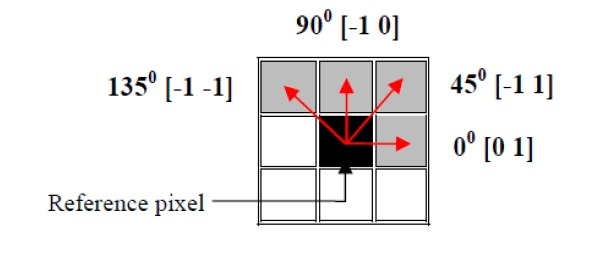
\includegraphics{GLCM_direction_sample}
\caption{GLCM angle directions for calculating textural features\cite{Biswajit}}
\end{figure}
In addition, by considering the symmetric property, the value of each element is doubled. In general, there is the fifth GLCM created by considering the average over created GLCM along with four angle directions. Offset means the distance between reference pixel value and its neighbor. Given $E_{(i,j)}$ which is the element in the array of pixels representing an image, if we consider $E_{(i,j)}$ as reference, the $E_{(i,j+n)}$ where n means the value of the offset is the neighbor in horizontal direction from left to right. Similarly, the the $E_{(i-n,j+n)}$ is the neighbor in diagonal direction from bottom left to top right, the $E_{(i-n,j)}$ is the neighbor in vertical direction from bottom to top, and the $E_{(i-n,j-n)}$ is the neighbor from bottom right to top left.\par
For example, given a 3-by-6 array  
\begin{align*}
I = 
\begin{bmatrix}
& 1 & 1 & 5 & 6 & 8 & 8 &\\
& 2 & 3 & 5 & 7 & 0 & 2 &\\
& 0 & 2 & 3 & 5 & 6 & 7 &
\end{bmatrix}
\end{align*}
it represents a sub-region of an image with pictorial information. GLCM is a m-by-m matrix where m is the gray levels of an image. For image I, since the pixel value ranges from 0 to 8, the gray level of image I is 9. Thus, a 9-by-9 matrix is created as a part of the whole GLCM in $0^0$ angle direction with offset 1. Under this circumstance, considering $E_{(1, 1)} = 1$ as the reference pixel value, its neighbor is $E_{(1, 2)} = 1$. Thus, the $G_{(1,1)}$ is currently equal to 1. In the meantime, we can find that the $G_{(0, 2)} = 2$, because when we treat the pixel value 0 as the reference, the pixel value 2 as the corresponding neighbor appears twice, which are $E_(2,6)$ and $E_(3,2)$.    
\begin{table}[!h]
\begin{center}
\renewcommand{\arraystretch}{0.5}
\begin{tabular}{c | c c c c c c c c c|}
 \backslashbox{\textit{reference}}{\textit{neighbor}} & 0 & 1 & 2 & 3 & 4 & 5 & 6 & 7 & 8 \\
\hline
 0 & 0 & 0 & 2 & 0 & 0 & 0 & 0 & 0 & 0 \\
 1 & 0 & 1 & 0 & 0 & 0 & 0 & 0 & 0 & 0 \\
 2 & 0 & 0 & 0 & 2 & 0 & 0 & 0 & 0 & 0 \\
 3 & 0 & 0 & 0 & 0 & 0 & 2 & 0 & 0 & 0 \\
 4 & 0 & 0 & 0 & 0 & 0 & 0 & 0 & 0 & 0 \\
 5 & 0 & 0 & 0 & 0 & 0 & 0 & 2 & 1 & 0 \\
 6 & 0 & 0 & 0 & 0 & 0 & 0 & 0 & 1 & 1 \\
 7 & 1 & 0 & 0 & 0 & 0 & 0 & 0 & 0 & 0 \\
 8 & 0 & 0 & 0 & 0 & 0 & 0 & 0 & 0 & 1 \\
\end{tabular}
\caption{The sub-region of GLCM in 0 degree (offset = 1)}
\end{center}
\end{table}
By counting all reference pixel values, we achieve the GLCM shown in Table 2.1. Similarly, we create the different GLCM in the rest three directions shown in Table 2.2, Table 2.3 and Table 2.4.
\begin{table}[!h]
\begin{center}
\renewcommand{\arraystretch}{0.5}
\begin{tabular}{c | c c c c c c c c c|}
 \backslashbox{\textit{reference}}{\textit{neighbor}} & 0 & 1 & 2 & 3 & 4 & 5 & 6 & 7 & 8 \\
\hline
 0 & 0 & 0 & 0 & 1 & 0 & 0 & 0 & 0 & 1 \\
 1 & 0 & 0 & 0 & 0 & 0 & 0 & 0 & 0 & 0 \\
 2 & 0 & 1 & 0 & 0 & 0 & 1 & 0 & 0 & 0 \\
 3 & 0 & 0 & 0 & 0 & 0 & 1 & 0 & 1 & 0 \\
 4 & 0 & 0 & 0 & 0 & 0 & 0 & 0 & 0 & 0 \\
 5 & 1 & 0 & 0 & 0 & 0 & 0 & 1 & 0 & 0 \\
 6 & 0 & 0 & 1 & 0 & 0 & 0 & 0 & 0 & 0 \\
 7 & 0 & 0 & 0 & 0 & 0 & 0 & 0 & 0 & 1 \\
 8 & 0 & 0 & 0 & 0 & 0 & 0 & 0 & 0 & 0 \\
\end{tabular}
\caption{The sub-region of GLCM in 45 degree (offset = 1)}
\end{center}
\begin{center}
\renewcommand{\arraystretch}{0.5}
\begin{tabular}{c | c c c c c c c c c|}
 \backslashbox{\textit{reference}}{\textit{neighbor}} & 0 & 1 & 2 & 3 & 4 & 5 & 6 & 7 & 8 \\
\hline
 0 & 0 & 0 & 1 & 0 & 0 & 0 & 0 & 0 & 1 \\
 1 & 0 & 0 & 0 & 0 & 0 & 0 & 0 & 0 & 0 \\
 2 & 0 & 1 & 0 & 1 & 0 & 0 & 0 & 0 & 1 \\
 3 & 0 & 1 & 0 & 0 & 0 & 1 & 0 & 0 & 0 \\
 4 & 0 & 0 & 0 & 0 & 0 & 0 & 0 & 0 & 0 \\
 5 & 0 & 0 & 0 & 0 & 0 & 1 & 0 & 1 & 0 \\
 6 & 1 & 0 & 0 & 0 & 0 & 0 & 0 & 0 & 0 \\
 7 & 0 & 0 & 1 & 0 & 0 & 0 & 1 & 0 & 0 \\
 8 & 0 & 0 & 0 & 0 & 0 & 0 & 0 & 0 & 0 \\
\end{tabular}
\caption{The sub-region of GLCM in 90 degree (offset = 1)}
\end{center}
\end{table}
\begin{table}
\begin{center}
\renewcommand{\arraystretch}{0.5}
\begin{tabular}{c | c c c c c c c c c|}
  \backslashbox{\textit{reference}}{\textit{neighbor}} & 0 & 1 & 2 & 3 & 4 & 5 & 6 & 7 & 8 \\
\hline
 0 & 0 & 0 & 0 & 0 & 0 & 0 & 1 & 0 & 0 \\
 1 & 0 & 0 & 0 & 0 & 0 & 0 & 0 & 0 & 0 \\
 2 & 0 & 0 & 1 & 0 & 0 & 0 & 0 & 0 & 1 \\
 3 & 0 & 1 & 0 & 1 & 0 & 0 & 0 & 0 & 0 \\
 4 & 0 & 0 & 0 & 0 & 0 & 0 & 0 & 0 & 0 \\
 5 & 0 & 1 & 0 & 0 & 0 & 1 & 0 & 0 & 0 \\
 6 & 0 & 0 & 0 & 0 & 0 & 0 & 0 & 1 & 0 \\
 7 & 1 & 0 & 0 & 0 & 0 & 1 & 0 & 0 & 0 \\
 8 & 0 & 0 & 0 & 0 & 0 & 0 & 0 & 0 & 0 \\
\end{tabular}
\caption{The sub-region of GLCM in 135 degree (offset = 1)}
\end{center}
\end{table}
For all tables from 2.1 to 2.4, the 
Finally, through adding these four GLCM together and dividing it by 4, we have the fifth GLCM.

\subsection{Texture Measurements of GLCM}
The texture measures of GLCM are calculated from the normalized GLCM. To achieve the normalized GLCM, each value in GLCM is divided by the total number of occurrences in the GLCM. Normally, the total number of occurrences is the amount of valid reference pixel. For instance, if we create the GLCM from the image I along with the $0^0$ direction with offset 1, the total number of occurrences is 15 because the reference pixels in the last column have no neighbors. Some basic functions will be used in calculating the texture features of GLCM\cite{Haralick}. Assuming that the parameter G represents the number of gray levels, the basic functions are defined as follow:\\
The probability of i as the reference pixel value in a gray-scale image:
\begin{equation}
    p_x(i) = \sum_{j=0}^{G-1}p(i,j) 
\end{equation}
The probability of j as the neighbor pixel value in a gray-scale image:
\begin{equation}
    p_y(j) = \sum_{i=0}^{G-1}p(i,j)
\end{equation}
The probability of k which is the summary of reference and neighbor pixel value:
\begin{equation}
    p_{x+y}(k) = \sum_{i=0}^{G-1}\sum_{j=0}^{G-1} p(i,j) \; where\; k = i + j\;(k=0,1,\ldots,2G-2)
\end{equation}
The probability of k which is the difference of reference and neighbor pixel value:
\begin{equation}
    p_{x-y}(k) = \sum_{i=0}^{G-1}\sum_{j=0}^{G-1} p(i,j) \; where\; k = |i - j|\;(k=0,1,\ldots,G-1)
\end{equation}
The mean value of $p_x$:
\begin{equation}
\mu_x = \sum_{i=0}^{G-1}ip_x(i)=\sum_{i=0}^{G-1}\sum_{j=0}^{G-1} ip(i,j)
\end{equation}
The standard deviation of $p_x$:
\begin{equation}
\sigma_x = \sqrt{\sum_{i=0}^{G-1}(i-\mu_x)^2p_x(i)}
\end{equation}
The mean value of $p_y$:
\begin{equation}
\mu_y = \sum_{j=0}^{G-1}jp_j(j)=\sum_{i=0}^{G-1}\sum_{j=0}^{G-1} jp(i,j)
\end{equation}
The standard deviation of $p_y$:
\begin{equation}
\sigma_y = \sqrt{\sum_{j=0}^{G-1}(j-\mu_y)^2p_y(j)}
\end{equation}
Consequently, due to the normalized GLCM and the basic functions listed above, the texture feature parameters of GLCM are defined as follow\cite{Haralick}:\\
1. Energy, Homogeneity, Angular Second Moment(ASM): 
\begin{equation}
ASM = \sum_{i=0}^{G-1}\sum_{j=0}^{G-1}\{p(i,j)\}^2
\end{equation}
The feature ASM is used to measure the homogeneity of an image\cite{Peng}. The value of ASM is usually more than $G^{-2}$ but less than 1. If a GLCM only has a few but relatively high value of $p(i,j)$, the homogeneous scene contains only a few gray levels\cite{Albregtsen}.\\
2. Inertia, Contrast(CON):
\begin{equation}
CON = \sum_{k=0}^{G-1}k^2p_{x-y}(k)
\end{equation}
The feature CON is used to measure the local difference within an image. Its value depends the position of pixel. In general, the more elements away from the diagonal, the higher value the feature has. Otherwise, the more elements in the diagonal, the lower value it has.\\ 
3. Correlation(COR):
\begin{equation}
COR = \frac{\sum_{i=0}^{G-1}\sum_{j=0}^{G-1}(i-\mu_x)(j-\mu_y)p(i,j)}{\sigma_x\sigma_y} = \frac{\sum_{i=0}^{G-1}\sum_{j=0}^{G-1}(ij)p(i,j)-\mu_x\mu_y}{\sigma_x\sigma_y}
\end{equation}
The feature COR is used to measure the linear dependence of gray levels between the specific position of pixels relative to each other. It depends how an image is organized. The value of COR is more than -1 but less than 1.\\
4. Sum of squares, variance(VAR):
\begin{equation}
VAR = \sum_{i=0}^{G-1}\sum_{j=0}^{G-1}(i-\mu_x)^2p(i,j) \\
    = \sum_{i=0}^{G-1}(i-\mu_x)^2p_x(i)
\end{equation}
The feature VAR measures the degree how the elements differ from the average value of $p(i,j)$. \\
5. Local Homogeneity, Inverse Difference Moment(IDM):
\begin{equation}
IDM = \sum_{i=0}^{G-1}\sum_{j=0}^{G-1}\frac{1}{1+(i-j^2)}p(i,j)
\end{equation}
The feature IDM is affected by the homogeneity of an image, because of the weighting factor $1+(i - j)^2$. Thus, the value is high if the image is homogeneous, while the value is low if the image is inhomogeneous.\\
6. Sum Average(SAV):
\begin{equation}
SAV = \sum_{k=0}^{2G-2}kp_{x+y}(k)
\end{equation}
7. Sum Entropy(SEN):
\begin{equation}
SEN = -\sum_{k=0}^{2G-2}p_{x+y}(k)\log(p_{x+y}(k))
\end{equation}
8. Sum Variance(SVA):
\begin{equation}
SVA = \sum_{k=0}^{2G-2}(k-SEN)^2p_{x+y}(k)
\end{equation}
9. Entropy(ENT)
\begin{equation}
ENT = - \sum_{i=0}^{G-1}\sum_{j=0}^{G-1}p(i,j)\log(p(i,j))
\end{equation}
10. Difference Entropy(DEN):
\begin{equation}
DEN = -\sum_{k=0}^{G-1}p_{x-y}(k)\log(p_{x-y}(k))
\end{equation}
11. Difference Variance(DVA):
\begin{equation}
DVA = \sum_{k=0}^{G-1}k^2p_{x-y}(k)
\end{equation}
12. Dissimilarity(DIS):
\begin{equation}
DIS = \sum_{i=0}^{G-1}\sum_{j=0}^{G-1}|i-j|p(i,j)
\end{equation}
13. Cluster shade(CLS):
\begin{equation}
CLS = \sum_{i=0}^{G-1}\sum_{j=0}^{G-1}(i+j-\mu_x-\mu_y)^3p(i,j) = \sum_{i=0}^{G-1}\sum_{j=0}^{G-1}(i+j-2\mu_x)^3p(i,j)
\end{equation}
14. Cluster prominence(CLP):
\begin{equation}
CLP=\sum_{i=0}^{G-1}\sum_{j=0}^{G-1}(i+j-\mu_x-\mu_y)^4p(i,j) = \sum_{i=0}^{G-1}\sum_{j=0}^{G-1}(i+j-2\mu_x)^4p(i,j)
\end{equation}
15. Minimum probability(MIP):
\begin{equation}
MIP = \min(p(i,j))
\end{equation}
16. Maximum probability(MAP):
\begin{equation}
MAP=max(p(i,j))
\end{equation}
17. Mean(MEA):
\begin{equation}
MEA = \sum_{i=0}^{G-1}i\sum_{j=0}^{G-1}p(i,j) = \mu_x
\end{equation}
18. relative minimum pixel intensity(IMIN):
\begin{equation}
IMIN = \frac{min(J(x,y))}{mean(J(x,y))}
\end{equation}
19. relative maximum pixel intensity(IMAX):
\begin{equation}
IMAX = \frac{max(J(x,y))}{mean(J(x,y))}
\end{equation}
20. Mean value of pixel intensity(IMEA):
\begin{equation}
IMEA = mean(J(x,y))
\end{equation}
where J(x,y) represents the 12-bit diffraction image before normalization. Based on Haralick's research\cite{Thati}, the texture features defined above are categorized into three groups named as \textit{Contrast}, \textit{Uniformity} or \textit{Orderliness} of pixels, and \textit{Correlation} and \textit{statistic} over the pixels. In Group 1, the measures of Contrast includes CON, DIS, IDM, VAR, SVA and DVA. In Group 2, the measures of Uniformity or Orderliness of pixels consist of MAP, ASM, ENT, DEN, SEN, CLS and CLP. In group 3, the measures of Correlation and other descriptive statistics contain COR, MIP, MEA, IMIN, IMAX, IMEA and SAV.\par
These feature parameters facilitate representing an image from the textural level. For example, given two different types of diffraction images taking both from camera with s-polarizer in front of as the Figure 2.2 shown, we examine three basic feature parameters from different group. The feature CON in group 1 describes the difference moment of image pixel matrix by measuring the amount of local variations present in an image. As for the images shown in Figure 2.2, the CON value of Cell image is 2.511395, while the value of Debris image is 104.8141, which is calculated using equation 2.10. The Debris image has larger CON value than the Cell image because the Cell image has less amount of local variations than the Debris image as the Figure 2.2 shown. The feature ASM in group 2 describes the degree of homogeneity that an image has by measuring the total number of dominant gray-tone transitions. Through calculation, the value of Cell image is 0.031834, whereas the value of Debris image is 0.000838. Due to the fact that the Cell image has very fewer dominant gray-tone transitions than the Debris image, the ASM of Cell image is higher than the Debris image. Another feature COR in group 3 describes the gray-tone linear-dependencies by considering the amount of linear structure across the image. The Debris image has lower value than the Cell image because the Debris image contains noise sample which is usually uncorrelated. In the meanwhile, by comparing the COR value of the Debris image along different directions, the values along $0^0$ and $90^0$ are higher than the values along $45^0$ and $135^0$ because the Debris image has a certain amount of linear structure along these two lines across it. 
\begin{figure}[!t]
\centering
  \begin{subfigure}[b]{0.4\textwidth}
    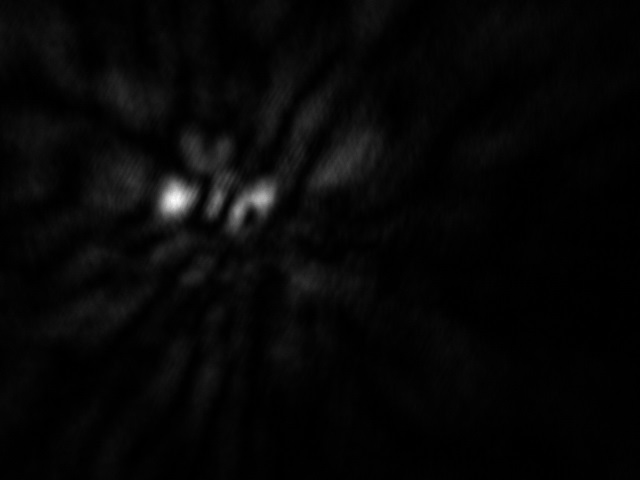
\includegraphics[width=\textwidth]{diffraction_image/2015040117594700116-2}
    \caption{Cell image}
  \end{subfigure}
  \begin{subfigure}[b]{0.4\textwidth}
    
\includegraphics[width=\textwidth]{diffraction_image/2015040117594700009-2}
    \caption{Debris image}
  \end{subfigure}
  \caption{Two diffraction images with different types captured with s-polarizer}
\end{figure}
\section{Development of GLCM Feature Calculation Application}
\subsection{Problem Statement}
Since the GLCM as a texture analysis approach is so popular, some tools provide the built-in method to create GLCM, such as MATLAB. However, for users who do not have the experience on MATLAB, it is hard for them to utilize the built-in method there. Even though users have little knowledge or experience of MATLAB, it is inconvenient to implement a script for extracting GLCM texture feature parameters. Thus, a developed application is necessary to be implemented. From the requirement perspective, the application shall allow users to specify the image folder so that the application can automatically process all images in that folder. The application also shall allow users to customize the offset value and the direction for creating the GLCM. To expand the function, the application should enable users to have the choices that the application presents feature parameters in single direction or combination of directions or the feature parameters normalized by all processed directions. Finally, the application shall automatically combine an image pair as a feature parameter example.  
\subsection{Class Diagram and GLCM Application Implementation}
\begin{figure}[!h]
\begin{center}
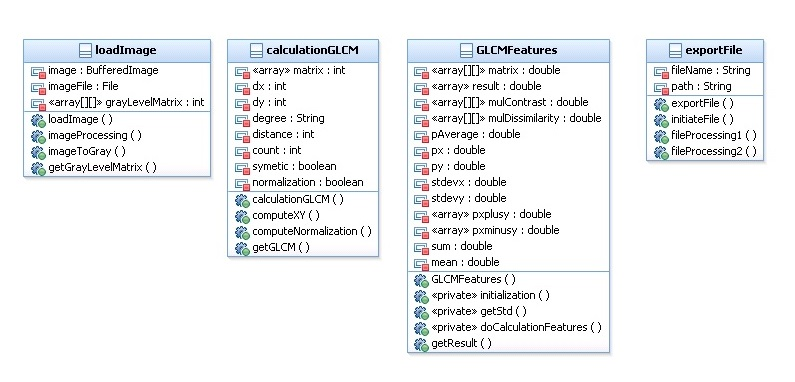
\includegraphics[width=4.25in]{class_diagram}
\end{center}
\renewcommand{\baselinestretch}{1}
\small\normalsize
\begin{quote}
\caption{The major classes for GLCM feature calculation application}
\label{fig2.2}
\end{quote}
\end{figure}
\renewcommand{\baselinestretch}{2}
\small\normalsize
Based on the problem statement above, the application should comprise several components which are loading images, converting into 2D matrix, computing GLCM based on the 2D matrix, calculating features from GLCM, and exporting comma-separated values (CSV) file that is used to store the desirable result. Therefore, the major classes shown in Figure 2.3 are constructed to represent the attributes and operations within the application. To process the massive amount of images, the application loops the procedure consisting of class loadImage, class calculationGLCM, and class GLCMFeatures until no image remained. During each loop, all calculated features are stored using ArrayList method. Finally, class exportFile extracts all features from ArrayList and conducts them into CSV file.\par
In this application, class loadImage is implemented by applying the Application Program Interface (API) Image I/O in JAVA library. The API provides a way loading the image into its BufferedImage formats. It supports with built-in methods for GIF, PNG, JPEG, BMP, and WBMP which are some different format of image data. In JAVA, the BufferedImage which is a subclass of Image class describes an image with an accessible buffer of image data. Within the BufferedImage class, it is constructed by the raster of image data that represents a rectangle array of pixels. Thus, through applying these APIs, the image data is processed and generate a rectangle array of pixels whose size is due to the resolution of the image. for example, if the resolution of an image is 640x480, the raster of the image data is a 640-by-480 array of pixels. In the meantime, the range of image pixel depends on its color depth. For instance, the highest pixel of an 8-bit image data is 256. \par
The calculationGLCM class takes the array of pixels that is the output of loadImage class as input and create the specific GLCM due to other input parameters such as distance and angular. The mechanism for this class is going through all elements in the array of pixels, and for each element, finding its corresponding neighbor element with specific conditions. Meanwhile, if an element has no neighbor, it contributes nothing to GLCM. As a result, given an m-by-n array of pixels
\begin{align*}
I = 
\begin{bmatrix}
E(0,0) & E(0,1) & \ldots & E(0,n-1) \\
\vdots &         &         & \vdots \\
E(d,0) & E(d,1) & \ldots & E(d,n-1) \\
\vdots &         &         & \vdots \\
E(m-1,0) & E(m-1,1) & \ldots & E(m-1,n-1) 
\end{bmatrix}
\end{align*} where d is the offset value and considering the exception problem in programming,
to calculate GLCM along 0 degree direction, a two dimension loop that counting the frequency starts from the element $E(0,0)$ and ends at the element $E(m-1, n-d)$; to calculate GLCM along 45 degree direction, the loop starts from the element $E(d,0)$ and ends at the element $E(m-1, n-d)$; to calculate GLCM along 90 degree direction, the loop starts from the element $E(d,0)$ and ends at the element $E(m-1, n-1)$; to calculate GLCM along 135 degree direction, the loop starts from the element $E(d,d)$ and ends at the element $E(m-1, n-1)$. 
By applying class GLCMFeatures, all texture features are calculated from the GLCM created through class calculationGLCM. In this class, the method initialization() is implemented to calculate parameters $p_x(i)$, $p_y(j)$, $p_{x+y}(k)$, $p_{x-y}(k)$, $\mu_x$, $\mu_y$, $\sigma_x$ and $\sigma_y$ due the equations from 2.1 to 2.8. Then, we implement the doCalculationFeatures() method that is responsible for calculating the 17 texture features of an image which are listed from equation 2.9 to 2.25.\par
Finally, the class exportFile is implemented for creating the result report in CSV format. General speaking, the common strategy is building a string with the comma. In this case, we utilize the StringBuilder method to construct the string in that format and apply the printWriter function to add it to a specific CSV file. 

\subsection{GLCM Application Verification}
Software verification as a part of software testing is an important procedure to ensure that the software is implemented all requirements. The two primary goals for software testing is finding bugs or defects and getting confidence in the software\cite{Jiantao}. Traditionally, the testing methods are divided into white-box testing that examines the internal structure or workings of a program and black-box testing that examines the functionality without knowing the internal implementation and seeing the source code. To do the black-box testing, test oracle which is a mechanism in software testing to determine whether a test has passed or not\cite{Kaner} is required. in the meanwhile, the test case which includes a set of test data as inputs, the expected outputs, and the execution condition is the central factor that is involved in the use of an oracle. As for the GLCM application, the input is an image and the output is the corresponding texture features based on the image's GLCM for system testing which is a high-level software testing process.
In this thesis research, there are MATLAB scripts implemented for research in selecting features to analyze the diffraction image\cite{Thati} and the C++ tool implemented for calculating texture features from GLCM. To verify them, we consider the black-box testing because tester lacks enough knowledge in MATLAB and C++ programming language. However, by using four diffraction images shown in Figure 2.4 as inputs for the testing process, the calculated texture features are different between these two tools. 
\begin{figure}[!b]
  \begin{subfigure}[b]{0.5\textwidth}
    
\includegraphics[width=\textwidth]{PicA1000}
    \caption{}
  \end{subfigure}
  \begin{subfigure}[b]{0.5\textwidth}
    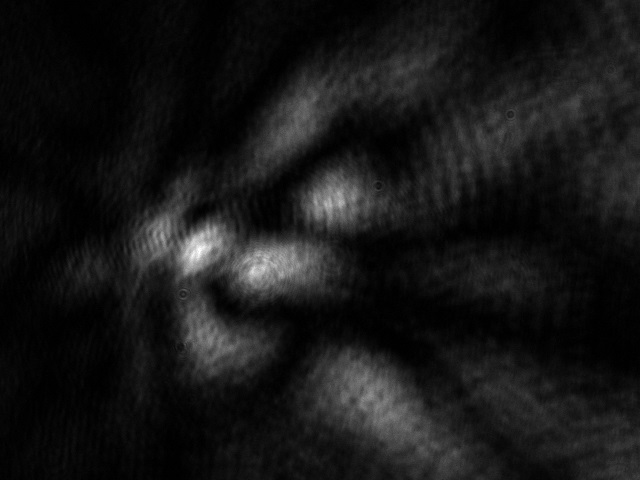
\includegraphics[width=\textwidth]{PicA1001}
    \caption{}
  \end{subfigure}
  \begin{subfigure}[b]{0.5\textwidth}
    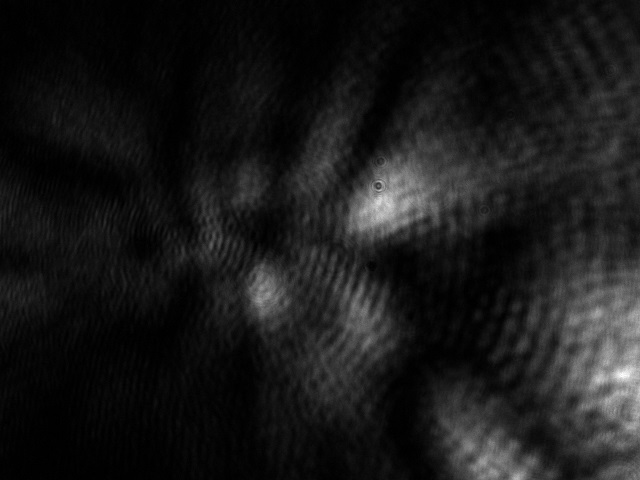
\includegraphics[width=\textwidth]{PicA1002}
    \caption{}
  \end{subfigure}
  \begin{subfigure}[b]{0.5\textwidth}
    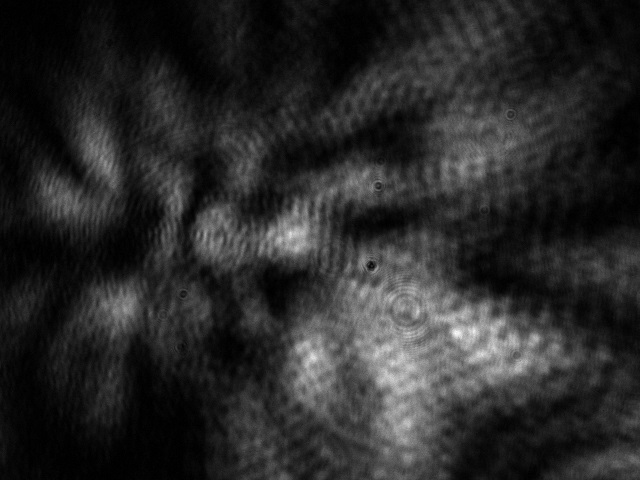
\includegraphics[width=\textwidth]{PicA1003}
    \caption{}
  \end{subfigure}
  \caption{The test input for verifying GLCM applications}
\end{figure}
In Table 2.5, we select five textural features from total 17 features to compare. Based on the comparison of results between MATLAB and C++, we can assume that either one of the code has or both of them have bugs or defects inside so that the requirements are not satisfied well. To prove, another application is implemented in JAVA, which is discussed in previous section, to verify the assumption proposed above. 
\begin{table}[!b]
\begin{center}
\begin{tabular}{||c c c ||}
& Image (a) & \\
\hline
Feature & MATLAB & C++ \\[0.7ex]
\hline\hline
COR & 0.985299 & 0.984588 \\
DIS & 2.20703 & 2.234017 \\
CON & 10.06387 & 10.63786 \\
IDM & 0.380147 & 0.407319 \\
ASM & 0.005497 & 0.013697 \\
\hline
\end{tabular}
\vspace{0.5cm}
\begin{tabular}{||c c c ||}
& Image (b) & \\
\hline
Feature & MATLAB & C++ \\[0.7ex]
\hline\hline
COR & 0.990801 & 0.990473 \\
DIS & 2.459202 & 2.487369 \\
CON & 12.97538 & 13.50661 \\
IDM & 0.364664 & 0.387451 \\
ASM & 0.003817 & 0.009142 \\
\hline
\end{tabular}
\begin{tabular}{||c c c ||}
& Image (c) & \\
\hline
Feature & MATLAB & C++ \\[0.7ex]
\hline\hline
COR & 0.991887 & 0.991633 \\
DIS & 2.626308 & 2.651188 \\
CON & 14.99225 & 15.53600 \\
IDM & 0.355747 & 0.380085 \\
ASM & 0.003739 & 0.009151 \\
\hline
\end{tabular}
\begin{tabular}{||c c c ||}
& Image (d) & \\
\hline
Feature & MATLAB & C++ \\[0.7ex]
\hline\hline
COR & 0.989492 & 0.989358 \\
DIS & 3.956470 & 3.969021 \\
CON & 30.91669 & 31.39502 \\
IDM & 0.254904 & 0.272799 \\
ASM & 0.001061 & 0.002534 \\
\hline
\end{tabular}
\caption {The feature values calculated from MATLAB and C++ for images in Figure 2.4}
\end{center}
\end{table}
At the beginning, the JAVA code is only implemented for calculating the COR, DIS, CON, IDM and ASM texture feature parameters for verification purpose. By using the same four diffraction images shown in Figure 2.4 as test inputs, we unfortunately got another version of result that is different from both MATLAB and C++. In Table 2.6, we present the comparison of result for Figure 2.4(a). 
\begin{table}[!t]
\begin{center}
\begin{tabular}{||c c c c||}
\hline
Feature & MATLAB & C++ & JAVA\\[0.7ex]
\hline\hline
COR & 0.985299 & 0.984588 & 0.962522 \\
DIS & 2.20703 & 2.234017 & 6.818101\\
CON & 10.06387 & 10.63786 & 82.14295 \\
IDM & 0.380147 & 0.407319 & 0.217207 \\
ASM & 0.005497 & 0.013697 & 0.005483\\
\hline
\end{tabular}
\caption{The texture feature results of Figure 2.4(a)}
\end{center}
\end{table}
From this result, we can't prove the assumption until we verify that the JAVA application is implemented to meet requirements. We apply the JUnit testing for major components comprising loadImage, calculationGLCM and GLCMFeatures. Consequently, we construct an 10-by-10 array of pixels ranging from 0 to 9 
\begin{align*}
I = 
\renewcommand{\arraystretch}{0.5}
\begin{bmatrix}
    1 & 6 & 2 & 3 & 9 & 3 & 0 & 6 & 2 & 8\\
    6 & 5 & 4 & 4 & 8 & 6 & 5 & 3 & 3 & 8\\
    0 & 9 & 7 & 0 & 0 & 6 & 8 & 2 & 6 & 7\\
    1 & 6 & 7 & 9 & 7 & 5 & 6 & 4 & 2 & 2\\
    5 & 7 & 1 & 2 & 2 & 6 & 2 & 4 & 7 & 5\\
    1 & 4 & 4 & 1 & 4 & 6 & 3 & 1 & 9 & 0\\
    7 & 4 & 5 & 3 & 5 & 2 & 4 & 5 & 7 & 4\\
    7 & 7 & 4 & 2 & 8 & 1 & 9 & 2 & 3 & 3\\
    7 & 1 & 6 & 4 & 4 & 9 & 1 & 3 & 5 & 1\\
    1 & 1 & 6 & 3 & 9 & 2 & 8 & 5 & 1 & 2
\end{bmatrix}
\end{align*}
as a test input to represent an image. By manually creating GLCM along 0 degree direction from the array of pixels, we achieve the GLCM
\begin{align*}
G_0 = 
\renewcommand{\arraystretch}{0.5}
\begin{bmatrix}
    1&     0&     0&     0&     0&     0&      2&     0&     0&     1\\
    0&     1&     2&     1&     2&     0&     4&     0&     0&     2\\
    0&     0&     2&     2&     2&     0&     2&     0&     3  &   0\\
    1&     1&     0&     2&     0&     2&     0&     0&     1 &    2\\
    0&     1&     2&     0&     3&     2&     1&     1 &    1  &   1\\
    0 &    2  &   1  &   2   &  1  &   0  &   1 &    2&     0  &   0\\
    0&     0&     3&     2&     2&     2&     0&     2&     1  &   0\\
    1&     2&     0&     0&     3&     2&     0&     1 &    0  &   1\\
    0 &    1  &   1   &  0   &  0  &   1 &    1&     0&     0  &   0\\
    1&     1&     2&     1&     0&     0&     0&     2&     0  &   0
\end{bmatrix}
\end{align*}
Based on the GLCM, we calculate the values of texture feature parameters COR, DIS, CON, IDM and ASM which are the expected outputs. Therefore, we create a test case including the test input I and expected output G for the JAVA application that is treated as execution condition. Through the verification process, we achieve the result shown in Table 2.7. 
\begin{table}[!h]
\begin{center}
\begin{tabular}{|| c | c  c | c ||}
\hline
Texture Feature & expected Result & Actual Result & Passed \\
\hline\hline
COR & 0.999965 & 0.999965 & Y \\
DIS & 290.0 & 290.0 & Y \\
CON & 1432.0 & 1432.0 & Y \\
IDM & 22.749199 & 22.749199 & Y\\
ASM & 174.0 & 174.0 & Y\\
\hline
\end{tabular}
\end{center}
\caption{Testing result for JAVA application}
\end{table}
As the table shown, all actual results are matched with expected results, which indicates the JAVA application can satisfy the requirements and achieve the correct feature values. To cover all possible GLCM created along all directions, we perform the same process for 45 degree, 90 degree and 135 degree angle and manually create the GLCM for the rest single direction:
\begin{align*}
G_{45} = 
\renewcommand{\arraystretch}{0.5}
\begin{bmatrix}
     0&     0&     0&     0&     0 &    1&     1&     0&     1&     0\\
     0&     2&     2&     0&     2 &    0&     1&     2&     0&     2\\
     0&     1&     0&     2&     1 &    2&     0&     3&     0&     0\\
     0&     0&     1&     1&     4 &    0&     0&     0&     1&     0\\
     0&     3&     2&     2&     1 &    0&     2&     0&     1&     1\\
     0&     1&     1&     1&     0 &    1&     3&     0&     1&     1\\
     1&     0&     3&     0&     1 &    1&     2&     1&     1&     0\\
     2&     0&     1&     0&     3 &    1&     1&     2&     0&     0\\
     0&     0&     1&     3&     0 &    0&     0&     0&     0&     0\\
     1&     0&     0&     0&     1 &    2&     0&     0&     0&     2
\end{bmatrix}
G_{90} = 
\begin{bmatrix}
     0&     0&     0&     0&     1&     1&     1&     0&     1&     0\\
     1&     1&     2&     1&     1&     2&     0&     3&     0&     1\\
     0&     1&     0&     2&     0&     1&     3&     2&     0&     2\\
     0&     1&     3&     0&     2&     0&     1&     1&     0&     0\\
     1&     1&     4&     2&     2&     1&     0&     1&     1&     0\\
     1&     2&     1&     2&     2&     0&     2&     0&     0&     0\\
     0&     1&     0&     2&     1&     1&     3&     0&     1&     1\\
     1&     1&     1&     0&     2&     0&     1&     3&     1&     1\\
     0&     1&     0&     0&     0&     2&     0&     0&     1&     1\\
     1&     1&     0&     0&     2&     1&     0&     1&     0&     0
\end{bmatrix}
\end{align*}
\begin{align*}
G_{135} = 
\renewcommand{\arraystretch}{0.5}
\begin{bmatrix}
     0&     0&     0&     0 &    2 &    0 &    0 &    1  &   0  &   0\\
     0&     2&     1&     2 &    0 &    1 &    1 &    2  &   0  &   0\\
     0&     0&     1&     0 &    3 &    4 &    1 &    1  &   0  &   1\\
     1&     0&     0&     0 &    1 &    1 &    3 &    1  &   0  &   1\\
     0&     1&     3&     0 &    2 &    1 &    3 &    1  &   1  &   1\\
     1&     3&     2&     2 &    1 &    0 &    0 &    0  &   0  &   0\\
     1&     1&     1&     1 &    0 &    0 &    1 &    2  &   1  &   1\\
     1&     2&     0&     1 &    1 &    1 &    0 &    1  &   0  &   1\\
     0&     0&     1&     2 &    0 &    0 &    1 &    0  &   0  &   1\\
     0&     0&     1&     0 &    2 &    0 &    1 &    1  &   1  &   0
\end{bmatrix}
\end{align*}
Based on these GLCM, we further create the average GLCM from all directions via dividing the sum for each element in GLCM by 4. The average GLCM is 
\begin{align*}
G_{ave} = 
\renewcommand{\arraystretch}{0.5}
\begin{bmatrix}
0.25 &0 &0 &0 &0.75 &0.5 &1 &0.25 &0.5 &0.25\\
0.25 &1.5 &1.75 &1 &1.25 &0.75 &1.5 &1.75 &0 &1.25\\
0 &0.5 &0.75 &1.5 &1.5 &1.75 &1.5 &1.5 &0.75 &0.75\\
0.5 &0.5 &1 &0.75 &1.75 &0.75 &1 &0.5 &0.5 &0.75\\
0.25 &1.5 &2.75 &1 &2 &1 &1.5 &0.75 &1 &0.75\\
0.5 &2 &1.25 &1.75 &1 &0.25 &1.5 &0.5 &0.25 &0.25\\
0.5 &0.5 &1.75 &1.25 &1 &1 &1.5 &1.25 &1 &0.5\\
1.25 &1.25 &0.5 &0.25 &2.25 &1 &0.5 &1.75 &0.25 &0.75\\
0 &0.5 &0.75 &1.25 &0 &0.75 &0.5 &0 &0.25 &0.5\\
0.75 &0.5 &0.75 &0.25 &1.25 &0.75 &0.25 &1 &0.25 &0.5
\end{bmatrix}
\end{align*}
Through operating the calculationGLCM method, all GLCM generated from JAVA application are the same as the expected results. 
Although we confirm that the texture features can be correctly calculated from GLCM, as well as that the GLCM can be created from the array of pixels, it is required to verify whether the array of pixels can represent the image correctly or not. Because of the complexity of image data, it is impossible to manually create the expected output for an image. Instead, we consider using a verified method to generate the expect output from image such as the imread() method in MATLAB. However, by comparing some elements with the same position in the matrix, the values are different. We pick 27-pixel values of image ranging from 10 to 255 in the matrix generated from the imread() method and choose the same number of the pixel value in the same position of a matrix created from JAVA application. Through building a map between each pixel value from MATLAB and its corresponding value from JAVA, we can obviously see the nonlinear line trend shown in Figure 2.5, 
\begin{figure}[!h]
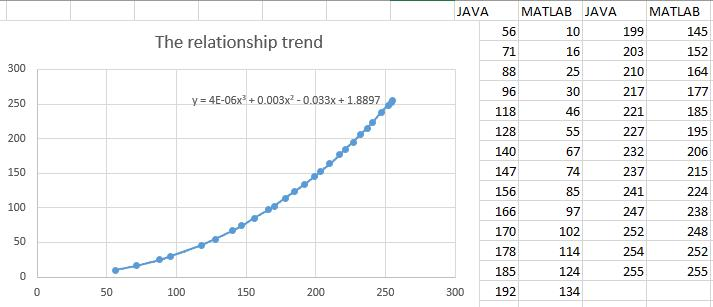
\includegraphics[width = \linewidth]{rgb_statistical}
\caption{The nonlinear relationship between JAVA and MATLAB result}
\end{figure}
which means we fail to create the correct pixel matrix from the image using JAVA application. Through some research, the misuse of the class Color is the reason of getting the wrong matrix. Instead of class Color, class Raster is the correct choice for a Gray-level image. The problem is caused by default color space sRGB, a proposed standard RGB color space, in Color class. Also, in BufferedImage class, the method getRGB() return an integer pixel in default color model TYPE\_INT\_ARGB, while the color model of our images is TYPE\_BYTE\_GRAY. Thus, we replace the Color class with the Raster class. After fixing the defects existing in loadingImage class, we use the Figure 2.4(a) as input to run JAVA application again and receive the new result shown in Table 2.8. 
\begin{table}[!t]
\begin{center}
\begin{tabular}{||c c c c||}
\hline
Feature & MATLAB & C++ & JAVA\\[0.7ex]
\hline\hline
COR & 0.985299 & 0.984588 & 0.985184 \\
DIS & 2.20703 & 2.234017 & 2.2324890\\
CON & 10.06387 & 10.63786 & 10.13244 \\
IDM & 0.380147 & 0.407319 & 0.375932 \\
ASM & 0.005497 & 0.013697 & 0.005439\\
\hline
\end{tabular}
\caption{The texture feature results of Figure 2.4(a) after modification}
\end{center}
\end{table}
From the result, we can see there are still three different version of feature result, but for JAVA application, all components have passed the verification process, and the all possible directions for creating GLCM are covered within the testing procedure. Thus, we can confirm the assumption that both C++ application and MATLAB script contain defects, and the JAVA application can be applied in the future research.

\section{Diffraction Images Pre-Classification and Feature Calculation}
In this experiment, we are provided 6000 diffraction images within which there are 3000 diffraction image pairs. Each image pair contains two diffraction images captured at the same time by two cameras with s-polarizer or p-polarizer placed separately in front of them. All diffraction images we use in the experiment are 8-bit color, so the gray levels of an image are 256 ranging from 0 to 255. In addition, the resolution of these images is 640x480. Thus, the array of pixels is a 640-by-480 matrix with that the maximum number of each element is 255. To identify, the diffraction image pair has the same name as the symbol (-) and different part (1 or 2) after the symbol. For instance, the 2015040718412300745-1.bmp means the p-polarized, whereas the 2015040718412300745-2.bmp means the s-polarized. There is some research using the similar approach to acquiring diffraction images, such as the classification of Jurkat T and Ramos B cells\cite{Feng} and the analysis of cellular objects through diffraction images\cite{Zhang}. \par
The primary goal of this research is to select a model to solve automated classification problem for these diffraction image data. In general, the common strategy is to train computer by using supervised learning algorithm in machine learning. By applying this approach, the computer can attain the ability that classifying massive amount of diffraction image data itself. However, for training process, we have to have the training data set labeled. Therefore, all 3000 diffraction image pairs are pre-classified visually into to three types, Cell, Debris, and Strip. Some image pairs for each group are shown in Figure 2.6, 2.7 and 2.8. 
\begin{figure}[!h]
\centering
  \begin{subfigure}[b]{0.2\textwidth}
    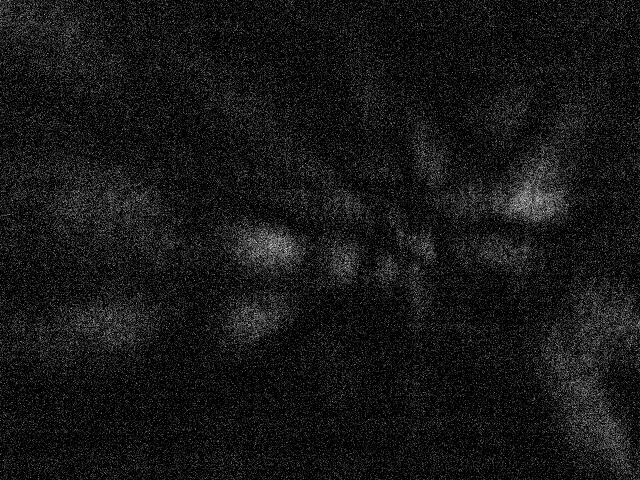
\includegraphics[width=\textwidth]{diffraction_image/2015040117594700171-1}
    \caption{p-polarizer}
  \end{subfigure}
  \begin{subfigure}[b]{0.2\textwidth}
    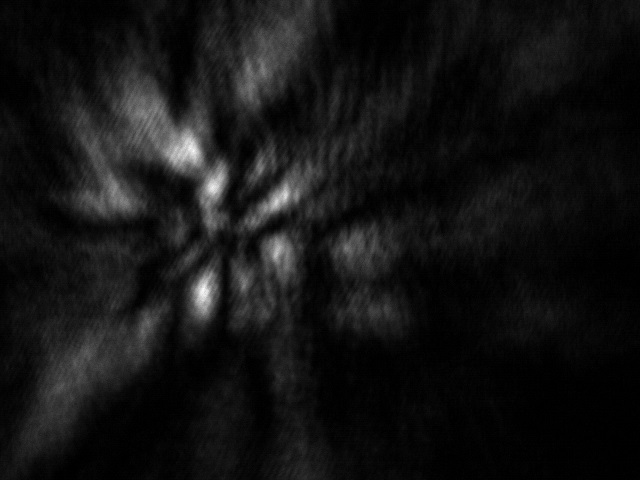
\includegraphics[width=\textwidth]{diffraction_image/2015040117594700171-2}
    \caption{s-polarizor}
  \end{subfigure}
  \begin{subfigure}[b]{0.2\textwidth}
    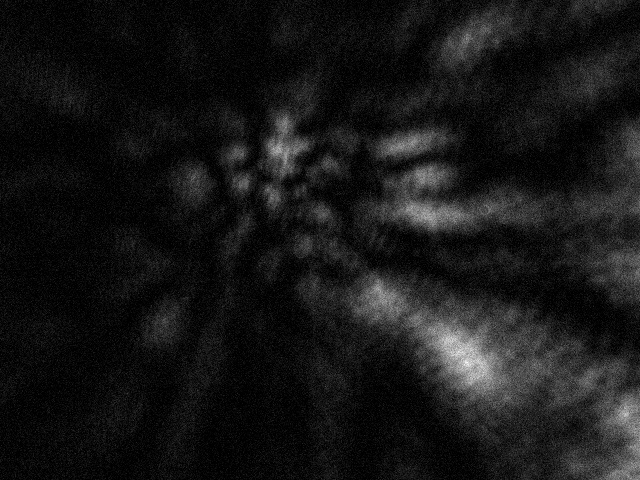
\includegraphics[width=\textwidth]{diffraction_image/2015040117594700185-1}
    \caption{p-polarizer}
  \end{subfigure}
  \begin{subfigure}[b]{0.2\textwidth}
    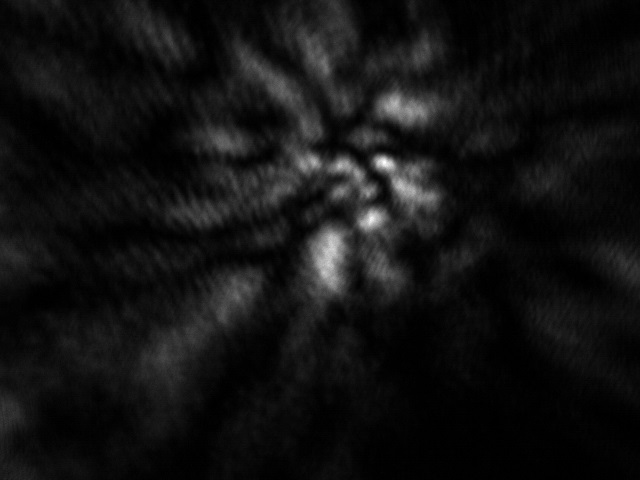
\includegraphics[width=\textwidth]{diffraction_image/2015040117594700185-2}
    \caption{s-polarizor}
  \end{subfigure}
  \caption{Diffraction images classified as Cell type}
\end{figure}
\begin{figure}[!h]
\centering
  \begin{subfigure}[b]{0.2\textwidth}
    
\includegraphics[width=\textwidth]{diffraction_image/2015040117594700004-1}
    \caption{p-polarizer}
  \end{subfigure}
  \begin{subfigure}[b]{0.2\textwidth}
    
\includegraphics[width=\textwidth]{diffraction_image/2015040117594700004-2}
    \caption{s-polarizor}
  \end{subfigure}
  \begin{subfigure}[b]{0.2\textwidth}
    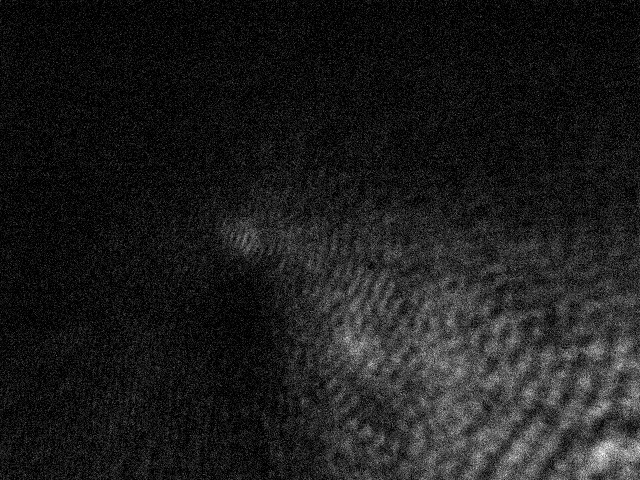
\includegraphics[width=\textwidth]{diffraction_image/2015040117594700050-1}
    \caption{p-polarizer}
  \end{subfigure}
  \begin{subfigure}[b]{0.2\textwidth}
    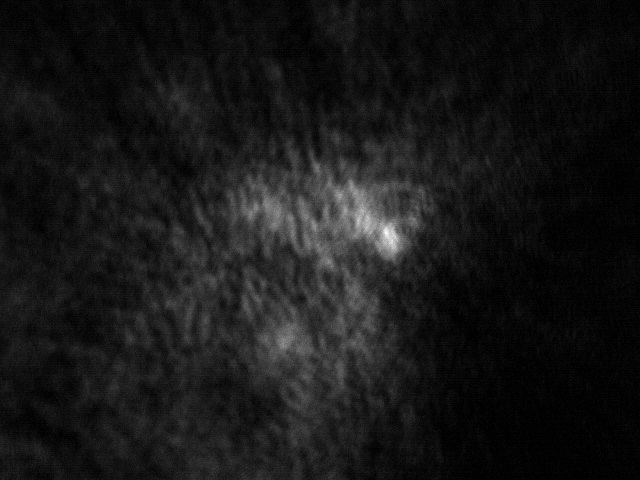
\includegraphics[width=\textwidth]{diffraction_image/2015040117594700050-2}
    \caption{s-polarizor}
  \end{subfigure}
  \caption{Diffraction images classified as Debris type}
\end{figure}
\begin{figure}[!h]
\centering
  \begin{subfigure}[b]{0.2\textwidth}
    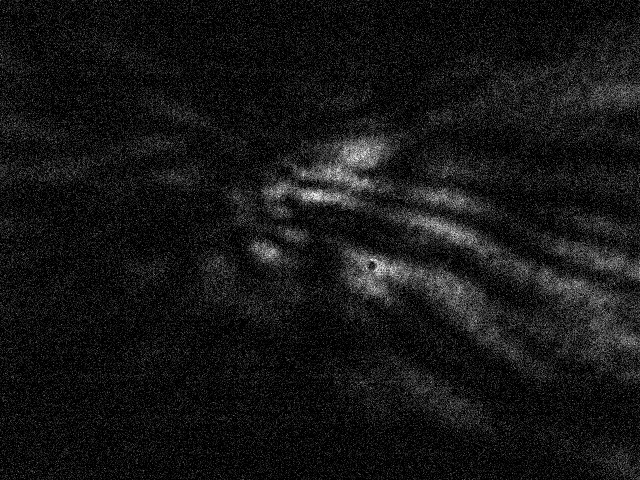
\includegraphics[width=\textwidth]{diffraction_image/2015040117594700071-1}
    \caption{p-polarizer}
  \end{subfigure}
  \begin{subfigure}[b]{0.2\textwidth}
    
\includegraphics[width=\textwidth]{diffraction_image/2015040117594700071-2}
    \caption{s-polarizor}
  \end{subfigure}
  \begin{subfigure}[b]{0.2\textwidth}
    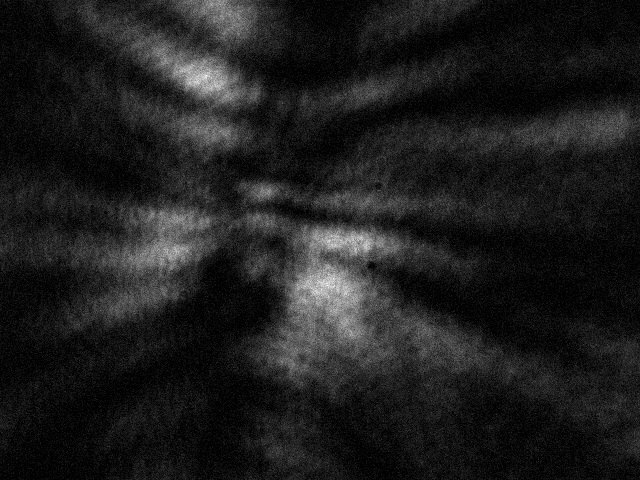
\includegraphics[width=\textwidth]{diffraction_image/2015040117594700158-1}
    \caption{p-polarizer}
  \end{subfigure}
  \begin{subfigure}[b]{0.2\textwidth}
    
\includegraphics[width=\textwidth]{diffraction_image/2015040117594700158-2}
    \caption{s-polarizor}
  \end{subfigure}
  \caption{Diffraction images classified as Strip type}
\end{figure}
Through the pre-classification process, we have 957 image pairs in Cell folder, 1555 image pairs in Debris folder, and 488 pairs in Strip folder. To process these image data, we operate the JAVA application and set up the offset and angular direction parameters shown in Figure 2.9. 
\begin{figure}
\centering
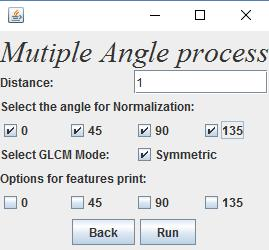
\includegraphics{java_panel}
\caption{JAVA application main panel}
\end{figure}
As it shown, the distance between two pixels is 1 and the application process the diffraction image data along with all directions. Because of having the symmetric checked, each value of an element in GLCM along each direction is doubled. In the meantime, the value of each element in GLCM is divided by the number of created GLCM, as well as normalized by the total amount of occurrences of valid reference pixel values. Eventually, the application generates three CSV files, Cell.CSV, Debris.csv, and Strip.csv, as the results that are used in the automated classification research later. 
\section{Conclusion}
In this section, we focus on the image texture analysis approach. As we discussed above, texture analysis is a common way to facilitate the analysis process. Within the texture analysis, GLCM is a popular and useful method to deal with the image texture analysis problems. It is proposed by Haralick\cite{Haralick} in 1973. The GLCM is created based on the spatial relations between two pixels of an image through counting the total number of occurrence of each pixel pair. The texture features are calculated from the GLCM to facilitate describing an image. In this research, we present the calculation of 20 texture features of images and apply 17 out of the total 20 features for automated classification experiment later. We implement JAVA application to verify MATLAB script and C++ tool but achieve three different versions of results. By applying black-box testing for all components of JAVA application, we confirmed the application has been implemented to meet all requirements. Through the operation of this application, all experiment image data are processed into texture features.  
%Chapter 3

\renewcommand{\thechapter}{3}

\chapter{Automated Classification for Diffraction Image Data}

\section{Overview}
In this research, we apply the supervised learning algorithm in machine learning to support image automated classification. In general, supervised learning conducts a model using a set of labeled training examples\cite{Mehryar}. Each example is a pair including an object as input and desired value as output. Typically, the input object is represented by M-by-N matrix where M is the number of training examples and N is the number of feature parameters in an example and the desired output value is called the supervisory signal. Thus, we construct the feature vector using the texture features calculated from GLCM and assign the desired output with diffraction image type which is cell, debris or strip. To realize supervised learning, there are lots of approaches and algorithms which are proposed and developed, such as support vector machine (SVM)\cite{Cortes}, artificial neural network\cite{McCulloch}, and so on.

\section{Support Vector Machine Algorithm}
Support Vector Machine (SVM) is a supervised learning model in machine learning for classification and regression analysis\cite{Cortes}. Given a set of labeled training data, the algorithm generates an optimal model which is able to be used to classify new examples. Therefore, given a set of training data of the form \{($x_1,y_1$),($x_2,y_2$),\ldots,($x_N,y_N$)\} where N is the number of examples in training data set, the major purpose of the SVM algorithm is to create a function 
\textit{f :} X $\rightarrow$ Y,
where $x_i$ $\in$ X (\textit{i} = 1,2,3,\ldots,N) is a training example with different feature parameters of an object and $y_i$ $\in$ Y is the output value corresponding to the $x_i$. For instance, the value of $y_i$ is sometimes either +1 or -1 for classification problem.   
\par
In SVM, the primary step is to achieve the hypothesis representation defined as 
\begin{equation}
    h_\theta(x) = \theta _0 + \theta_1x_1 + \theta_2x_2 + \theta_3x_3 + \dots + \theta_nx_n 
\end{equation}
where $x_n$ is the value of $n^{th}$ feature parameter in the training example. By considering the definition of matrix multiplication, the hypothesis representation also can be represented as 
\begin{equation}
    h_\theta(x) = 
    \begin{bmatrix}
        \theta_0 & \theta_1 & \dots & \theta_n
    \end{bmatrix}
    \begin{bmatrix}
        x_0\\
        x_1\\
        \vdots\\
        x_n
    \end{bmatrix}
    = \theta^Tx
\end{equation}
where $x_0$ normally equals to 1 from computation perspective. Once we achieved the hypothesis function, we can translate the output of the hypothesis function as follow 
\begin{equation}
     y=\left\{
  \begin{array}{@{}ll@{}}
    1, & \text{if}\ h_\theta(x) \geq 1 \\
    -1, & \text{if}\ h_\theta(x) \leq -1
  \end{array}\right.
\end{equation}
to get the discrete -1 or 1 classification. Due to the circumstance, the line that separates the area where y = 1 and where y = -1 is called decision boundary. Figure 3.1 is a instance of the decision boundary. Taking spam classification for email as an example, we create a set of training examples by converting each email into a feature vector $x \in R^n$ through referring the vocabulary list. For this example, n is the number of words in vocabulary list, and the feature $x_i\in {0,1}$ for an email depends on whether or not the $i^{th}$ word appears in the email. Given the label y $\in \{1, -1\}$, the corresponding feature vector looks like 
\begin{figure}[!b]
    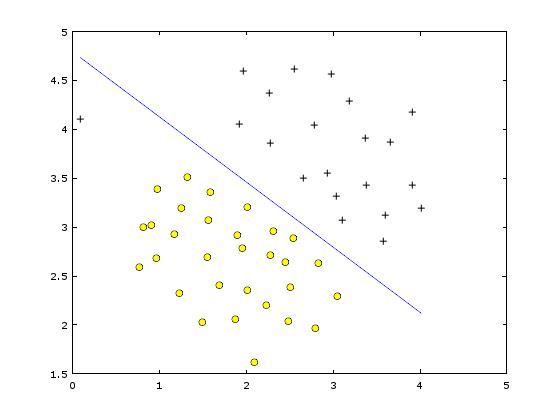
\includegraphics[width = \linewidth]{Fig1}
    \caption{A decision boundary that separates two class areas}
    \label{fig3.1}
\end{figure}
\begin{align*}
x = 
\renewcommand{\arraystretch}{0.4}
\begin{bmatrix}
        & 0 &\\
        & \vdots &\\
        & 1 &\\
        & 0 &\\
        & \vdots &\\
        & 0 &\\
        & 1 &\\
        & \vdots &\\
        & 0 &
    \end{bmatrix}
    \in R^n
\end{align*}
By training SVM classifier on multiple data like this, we can achieve a model which is able to predict the new example either the spam-email or the nonspam-email.\par   
However, the decision boundary may not be linear line in most of time. In order to solve more complex and non-linear classification problem, the kernel method is proposed in SVM to create the corresponding classifier. Given training set ($x^{(1)}$, $y^{(1)}$), ($x^{(2)}$, $y^{(2)}$), \ldots, ($x^{(m)}$, $y^{(m)}$), we choose 
\begin{align*}
    l^{(1)} = x^{(1)}, l^{(2)} = x^{(2)}, \ldots, l^{(m)} = x^{(m)}
\end{align*}
Due to the circumstance, an example x is given so that we can have
\begin{align*}
    f_1 = similarity(x, l^{(1)})\\
    f_2 = similarity(x, l^{(2)})\\
    \dots 
\end{align*}
As a result, we can build a map as follow
\begin{align*}
    g: x^{(i)} \rightarrow 
    \begin{bmatrix}
        f_1^{(i)} \\
        f_2^{(i)} \\
        \dots \\
        f_m^{(i)} \\
    \end{bmatrix}
\end{align*}
where $f_i^{(i)}$ = similarity($x^{(i)}$, $l^{(i)}$) = K($x^{(i)}$, $l^{(i)}$) that is the representation of the kernel.\par
In addition, the SVM algorithm can be applied in not only binary classification, but also multiple-class classification. To solve multiple-class classification problem, a common approach called one-vs-all is introduced. the one-vs-all approach is evolved from binary classification approach by considering the fact that the multiple-class classification problem can be considered as n+1 binary classification problem. For example, we can assume that we have a set of class data y $\in$ \{0, 1, 2, $\ldots$, n\} where n means the number of classes in the data. By considering it as n+1 binary classification problem, we can select one class and then group all the others into a single second class. We predict the probability of each selecting class through the formula as follow:
\begin{align*}
    {h_\theta}^{(0)}(x) = P (y = 0 | x ;\theta)\\
    {h_\theta}^{(1)}(x) = P (y = 1 | x ;\theta)\\
    \ldots \ldots \ldots \ldots\\
    {h_\theta}^{(n)}(x) = P (y = n | x ;\theta)
\end{align*}
Eventually, after repeating the process for all classes, we can achieve the highest value as prediction via using the hypothesis as follow:
\begin{align*}
    prediction = max ({h_\theta}^{(i)}(x))
\end{align*}
As a result, the SVM algorithm can solve the classification problem with more than two classes via one-vs-all approach.

\section{The Integrated Tool for SVM Classifier}
LIBSVM is a very useful integrated software for SVM algorithm\cite{Chang}. In LIBSVM, there are four basic kernels involved in LIBSVM which is an integrated software using SVM algorithm for classification, regression, and distribution estimation. Linear kernel, which is also called SVM without kernel, is represented as 
\begin{align*}
K(x^{(i)}, l^{(i)}) = {x^{(i)}}^Tl^{(i)}
\end{align*}
Polynomial kernel is represented as 
\begin{align*}
K(x^{(i)}, l^{(i)}) = (\gamma{x^{(i)}}^Tl^{(i)} + r)^d
\end{align*}
Radial basis function (RBF) is represented as 
\begin{align*}
K(x^{(i)}, l^{(i)}) = \textbf{exp}(-\gamma*\|x^{(i)} - l^{(i)}\|^2)
\end{align*}
Finally, sigmoid kernel is represented as 
\begin{align*}
K(x^{(i)}, l^{(i)}) = \textbf{tanh}(\gamma{x^{(i)}}^Tl^{(i)} + r)
\end{align*}
In LIBSVM, the default value for $\gamma$, r and d are $\gamma$=1/number\_features, r = 0 and d = 3. 
\par
Since kernel plays a significant part in SVM, selecting the best kernel for solving classification or regression problem is extremely important. In LIBSVM, the RBF kernel is normally the first choice using for SVM classifier. As it described, the advantages of choosing RBF kernel include, firstly, it can handle nonlinear relationship between class labels and features; secondly, the RBF kernel has less hyperparameters which affects the complexity of selecting model than the polynomial kernel; finally, the RBF kernel has fewer numerical difficulties.
\par
However, it is not always the case that uses the RBF kernel for SVM classifier. If the number of features is larger than the number of training examples, there is no need to map the data to a higher dimensional space. As a result, it is much wiser to consider the linear kernel instead of the RBF kernel. \par

We apply LIBSVM for our current research because it provides multiple interfaces, such as Python, MATLAB, Ruby, PHP, and so on, for users to integrate the tool into their own application for solving classification problem, instead of developing it from scratch. In our research, we consider integrating LIBSVM into MATLAB to deal with the 3-class classification problem.\par
In general, the LIBSVM tool has the following procedure:
\begin{itemize}
\item Prepare data to the format of an SVM package
\item Simply scale data for each feature parameter
\item Consider the RBF kernel
\item Find the best parameter C and $\gamma$
\item validate the selected SVM classifier
\end{itemize}
Within the procedure above, the parameter C comes from the solution of the following optimization problem:
\begin{align}
    \min\limits_{w,b,\xi}\;\; \frac{1}{2}w^Tw + C\sum_{i=1}^{l}\xi_i\nonumber \\subject\;to\;\;y_i(w^T\phi(x_i)+b) \geq 1 - \xi_i,\\\xi_i\geq0\nonumber
\end{align}


\section{Experimental Method and Result}
\subsection{Experimental Data Preprocessing}
In chapter 2, we discussed a statistic method GLCM as well as its texture features, and a JAVA application is developed to create the GLCM and calculate the texture feature parameters. During that experimental procedure, there are 6000 diffraction images that are processed and 3000 feature vectors that are achieved. In this research, 17 texture features are estimated to classify diffraction images. Thus, the feature vector contains 34 features and is represented as follow:
\begin{align*}
x = 
\renewcommand{\arraystretch}{0.5}
\begin{bmatrix}
    & s-ASM & \\
    & s-CON & \\
    & \vdots & \\
    & s-MEA & \\
    & p-ASM & \\
    & \vdots & \\
    & p-MAP & \\
    & p-MEA & 
\end{bmatrix}
\in R^{34}
\end{align*}
By categorizing each feature vector with label y $\in {1,2,3}$, the $n^{th}$ data example is presented as $(x_n,y_n)$. The whole experimental data comprise massive amount of data examples, and some data examples are presented in Table 3.1.
\begin{table}[!h]
\renewcommand{\arraystretch}{0.5}
\begin{tabular}{||c c | c c c c c c c||}
\hline
& & & & & s-polarizer & & &\\
\hline
Index & Label & ASM & CON & $\cdots$ & ENT & $\cdots$ & MAP & MEA\\[0.7ex]
\hline\hline
1 & 1(Cell) & 0.005231 & 12.80734 & $\cdots$ & 6.083719 & $\cdots$ & 0.017720 & 15.59143 \\
2 & 2(Debris) & 0.005735 & 23.77143 & $\cdots$ & 6.521346 & $\cdots$ & 0.040336 & 21.52553 \\
3 & 3(Strip) & 0.001789 & 173.6012 & $\cdots$ & 7.801943 & $\cdots$ & 0.029414 & 35.95368 \\
4 & 2(Debris) & 0.000877 & 48.90878 & $\cdots$ & 7.634998 & $\cdots$ & 0.003237 & 32.81473 \\
5 & 1(Cell) & 0.007662 & 10.50349 & $\cdots$ & 5.847001 & $\cdots$ & 0.032482 & 14.93335 \\
$\cdots$ & $\cdots$ & $\cdots$ & $\cdots$ & $\cdots$ & $\cdots$ & $\cdots$ & $\cdots$ & $\cdots$\\
\hline
\end{tabular}
\begin{tabular}{||c c | c c c c c c c||}
\hline
& & & & & p-polarizer & & &\\
\hline
Index & Label & ASM & CON & $\cdots$ & ENT & $\cdots$ & MAP & MEA\\[0.7ex]
\hline\hline
1 & 1(Cell) & 0.017970 & 318.8146 & $\cdots$ & 5.593921 & $\cdots$ & 0.107508 & 22.90067 \\
2 & 2(Debris) & 0.009067 & 35.29935 & $\cdots$ & 6.045092 & $\cdots$ & 0.057153 & 13.01318 \\
3 & 3(Strip) & 0.002249 & 11.78266 & $\cdots$ & 6.730682 & $\cdots$ & 0.006889 & 31.97666 \\
4 & 2(Debris) & 0.002810 & 380.3817 & $\cdots$ & 6.747705 & $\cdots$ & 0.029754 & 35.74588 \\
5 & 1(Cell) & 0.024522 & 210.0059 & $\cdots$ & 5.184235 & $\cdots$ & 0.128860 & 15.44677 \\
$\cdots$ & $\cdots$ & $\cdots$ & $\cdots$ & $\cdots$ & $\cdots$ & $\cdots$ & $\cdots$ & $\cdots$\\
\hline
\end{tabular}
\caption {The data examples consisting of feature vector and label vector}
\end{table}
In addition, it is very important for data preprocessing to scale features into the specific range. The primary advantage of this is to prevent the features in larger numerical ranges from dominating those in smaller numerical ranges. In general, features are linearly scaled into range $[-1, 1]$ or $[0, 1]$. In this research, we scale the values of each feature in the whole experimental data into range $[0,1]$. By applying the method, all experimental data are scaled as Table 3.2 shown. 
\begin{table}[!h]
\renewcommand{\arraystretch}{0.5}
\begin{tabular}{||c c | c c c c c c c||}
\hline
& & & & & s-polarizer & & &\\
\hline
Index & Label & ASM & CON & $\cdots$ & ENT & $\cdots$ & MAP & MEA\\[0.7ex]
\hline\hline
1 & 1(Cell) & 0.137243 & 0.063841 & $\cdots$ & 0.425415 & $\cdots$ & 0.144437 & 0.156314 \\
2 & 2(Debris) & 0.151231 & 0.127675 & $\cdots$ & 0.523982 & $\cdots$ & 0.351240 & 0.271903 \\
3 & 3(Strip) & 0.041784 & 1 & $\cdots$ & 0.812410 & $\cdots$ & 0.251371 & 0.552946 \\
4 & 2(Debris) & 0.016477 & 0.274027 & $\cdots$ & 0.774810 & $\cdots$ & 0.012014 & 0.491803 \\
5 & 1(Cell) & 0.204676 & 0.050428 & $\cdots$ & 0.372099 & $\cdots$ & 0.279424 & 0.143495 \\
$\cdots$ & $\cdots$ & $\cdots$ & $\cdots$ & $\cdots$ & $\cdots$ & $\cdots$ & $\cdots$ & $\cdots$\\
\hline
\end{tabular}
\begin{tabular}{||c c | c c c c c c c||}
\hline
& & & & & p-polarizer & & &\\
\hline
Index & Label & ASM & CON & $\cdots$ & ENT & $\cdots$ & MAP & MEA\\[0.7ex]
\hline\hline
1 & 1(Cell) & 0.223629 & 0.119862 & $\cdots$ & 0.385473 & $\cdots$ & 0.419955 & 0.039849 \\
2 & 2(Debris) & 0.110118 & 0.012186 & $\cdots$ & 0.476774 & $\cdots$ & 0.218175 & 0.039849 \\
3 & 3(Strip) & 0.023185 & 0.003255 & $\cdots$ & 0.615512 & $\cdots$ & 0.016762 & 0.241881 \\
4 & 2(Debris) & 0.030345 & 0.143244 & $\cdots$ & 0.618957 & $\cdots$ & 0.108382 & 0.282038 \\
5 & 1(Cell) & 0.307159 & 0.078537 & $\cdots$ & 0.302568 & $\cdots$ & 0.505513 & 0.065776 \\
$\cdots$ & $\cdots$ & $\cdots$ & $\cdots$ & $\cdots$ & $\cdots$ & $\cdots$ & $\cdots$ & $\cdots$\\
\hline
\end{tabular}
\caption {The scaled data examples consisting of feature vector and label vector}
\end{table}
Finally, the texture feature MIP is eliminated from the experimental data because the minimum probability of all diffraction images in in experimental data set is always 0. Consequently, 16 texture features including ASM, CON, COR, VAR, IDM, SAV, SEN, SVA, ENT, DEN, DVA, DIS, CLS, CLP, MAP and MEA are estimated for expressing an image. Since a feature vector is comprised two images separately captured by camera using either p-polarizer or s-polarizer, it contains 32 texture features as attribute parameters.    
\subsection{Feature Selection and Classifier Validation}
Through preprocessing the experimental data, we achieved a 3000-by-33 matrix. However, whether or not these texture features can be used for classification is unknown. If we use a invalid feature parameter for classification, the accuracy may be affected negatively. Thus, it is necessary to select valid features used by SVM for classification. In this research, we firstly propose a forward propagation approach that adding new feature as attribute parameter into existing attributes used by SVM and monitoring the accuracy variation of SVM classifier. By applying the approach, we start with training the SVM classifier on data with single attribute. Thus, we evolve a n-by-2 matrix from the n-by-33 matrix which may look like
\begin{align*}
X = 
\renewcommand{\arraystretch}{0.5}
\begin{bmatrix}
 & y_1 & x_1^{(1)} & \\
 & y_2 & x_2^{(1)} & \\
 & y_3 & x_3^{(1)} & \\
 & $\ldots$ & $\ldots$ \\
 & y_{n-1} & x_{n-1}^{(1)} & \\
 & y_n & x_n^{(1)} & \\
\end{bmatrix}
\end{align*}
where $x^{(1)}$ represents one of the 32 texture features. For instance, if we examine the accuracy of texture feature s-ASM, $x^{(1)}$ is the value of feature s-ASM. Therefore, the matrix of experimental data set should be 
\begin{align*}
X = 
\renewcommand{\arraystretch}{0.5}
\begin{bmatrix}
 & 1 & 0.137243 & \\
 & 2 & 0.151231 & \\
 & 3 & 0.041784 & \\
 & $\ldots$ & $\ldots$ \\
 & 2 & 0.016477 & \\
 & 1 & 0.204676 & \\
\end{bmatrix}
\end{align*}
By adding one more feature, the experimental data matrix is 
\begin{align*}
X = 
\renewcommand{\arraystretch}{0.5}
\begin{bmatrix}
 & y_1 & x_1^{(1)} & x_1^{(2)} &\\
 & y_2 & x_2^{(1)} & x_2^{(2)} &\\
 & y_3 & x_3^{(1)} & x_3^{(2)} &\\
 & $\ldots$ & $\ldots$ & $\ldots$\\
 & y_{n-1} & x_{n-1}^{(1)} & x_{n-1}^{(2)} &\\
 & y_n & x_n^{(1)} & x_n^{(2)} &\\
\end{bmatrix}
\end{align*}
By following the steps, we can find the highest accuracy of SVM classifier. When the accuracy reaches the peak, all the added feature parameters are the attribute parameters used by SVM for classification. In general, the experimental data matrix is represented as 
\begin{align*}
X = 
\renewcommand{\arraystretch}{0.5}
\begin{bmatrix}
 & y_1 & x_1^{(1)} & x_1^{(2)} & $\ldots$ & x_1^{(m)} & \\
 & y_2 & x_2^{(1)} & x_2^{(2)} & $\ldots$ & x_2^{(m)} &\\
 & y_3 & x_3^{(1)} & x_3^{(2)} & $\ldots$ & x_3^{(m)} &\\
 & $\ldots$ & $\ldots$ & $\ldots$ & $\ldots$\\
 & y_{n-1} & x_{n-1}^{(1)} & x_{n-1}^{(2)} & $\ldots$ & x_{n-1}^{(m)} &\\
 & y_n & x_n^{(1)} & x_n^{(2)} & $\ldots$ & x_n^{(m)} &\\
\end{bmatrix}
\end{align*}
Since the diffraction image is so abstract that the manual pre-classification process can't guarantee the accuracy. Thus, we manually select 200 data examples by experience from each type of diffraction image to reduce the risk that ambiguous diffraction images affect the accuracy of SVM classifier. As for the 600 examples in total, they are divided into three part, the training data set, the validating data set and the testing data set. We select 120 data examples from each type as the training data, 20 data examples from each type as the validating data, and 60 data examples from each type as the testing data. Thus, we have 360 examples in training set, 60 examples in validating set, as well as 180 examples in testing set. We apply one feature parameter in SVM and achieve the accuracy as Table 3.3 shown.  
\begin{table}[!t]
\begin{center}
\renewcommand{\arraystretch}{0.5}
\begin{tabular}{||c c c c c c ||}
\hline
Index & Feature & Accuracy & Index & Feature & Accuracy \\[0.7ex]
\hline\hline
1 & s-ASM & 32.22\% & 21 & p-ASM & 53.33\% \\
2 & s-CON & 35.00\% & 22 & p-CON & 30.00\% \\
3 & s-COR & 32.78\% & 23 & p-COR & 51.11\% \\
4 & s-VAR & 40.00\% & 24 & p-VAR & 41.11\% \\
5 & s-IDM & 37.78\% & 25 & p-IDM & 44.44\% \\
6 & s-SAV & 38.33\% & 26 & p-SAV & 44.44\% \\
7 & s-SEN & 32.78\% & 27 & p-SEN & 52.78\% \\
8 & s-SVA & 35.56\% & 28 & p-SVA & 37.78\% \\
9 & s-ENT & 35.00\% & 29 & p-ENT & 53.89\% \\
10 & s-DEN & 41.67\% & 30 & p-DEN & 42.78\% \\
11 & s-DVA & 36.11\% & 31 & p-DVA & 43.89\% \\
12 & s-DIS & 41.67\% & 32 & p-DIS & 26.67\% \\
13 & s-CLS & 39.44\% & 33 & p-CLS & 36.11\% \\
14 & s-CLP & 37.22\% & 34 & p-CLP & 35.00\% \\
16 & s-MAP & 30.56\% & 36 & p-MAP & 52.78\% \\
17 & s-MEA & 38.33\% & 37 & p-MEA & 44.44\% \\
\hline
\end{tabular}
\caption {The accuracy of the SVM classifier trained on 360 experimental data with single feature parameter}
\end{center}
\end{table}
The result indicates that the classifier may achieve better performance by using some features such as p-ASM, p-COR and p-ENT, while the classifier may achieve worse performance by using some features such as s-MAP, p-CON and p-DIS. To support the statement above, the Figure 3.2 shows a confusion matrix when the accuracy is 33.33\%. 
\begin{figure}[!h]
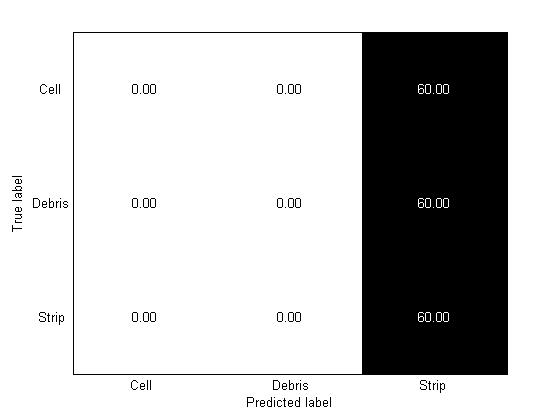
\includegraphics[width=\linewidth]{confusion_matrix/fig3_2}
\caption{A confusion matrix example when the accuracy is 33.33\%}
\end{figure}
As it illustrated, all testing data are classified as strip type. In the meantime, the probabilities of three classes are 0 for each testing example. In previous section, we mentioned that the mechanism of multiple class classification is applying the one-vs-all method and selecting the maximum probability of class as the predicted result. Thus, when the accuracy is 33.33\%, the achieved classifier doesn't work for classification. The classifier with accuracy 33.33\% is achieved by using feature s-MIP and p-MIP. Thus, we eliminate these two features. As Table 3.3 shown, the classifier can achieve the accuracy that is more than 50.00\% using feature p-ASM, p-COR, p-SEN, p-ENT, and p-MAP. Based on THE five features, we examine the remaining texture features and select six significant results shown in Table 3.4.   
\begin{table}[!h]
\begin{center}
\renewcommand{\arraystretch}{0.5}
\begin{tabular}{|| c | c c c ||}
\hline
 Feature Combination& p-ENT\&p-CON & p-ASM\&s-CLS & p-SEN\&p-CON \\
 \hline
 Accuracy & 57.78\% & 57.22\% & 57.22\% \\
 \hline
 Confusion Matrix & Figure 3.3(a) & Figure 3.3(b) & Figure 3.3(c) \\
 \hline
 \hline
 Feature Combination& p-ASM\&p-DIS & p-MAP\&p-CON & p-ASM\&p-CON \\
 \hline
 Accuracy & 57.22\% & 57.22\% & 56.67\% \\
 \hline
 Confusion Matrix & Figure 3.3(d) & Figure 3.3(e) & Figure 3.3(f) \\
 \hline
\end{tabular}
\end{center}
\caption{The accuracy of SVM classifier trained on data set with two feature parameters}
\end{table}
Due to the result, the accuracy is increased by adding one more feature. Especially, by comparing Table 3.4 with Table 3.3, we achieve a fact that the feature parameter contributing low accuracy is able to improve the performance of the classifier using another feature contributing a high accuracy. For example, when training the classifier on the data with feature parameter p-DIS, the accuracy is 26.67\%. However, by training the classifier on the data with the feature combination consisting of p-DIS and p-ASM, the accuracy is 57.22\% which is higher than the accuracy of the classifier trained on data only with the feature parameter p-ASM. 
\begin{figure}[!h]
\centering
  \begin{subfigure}[b]{0.3\textwidth}
    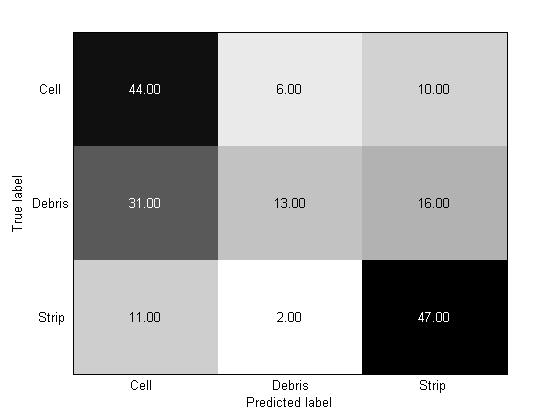
\includegraphics[width=\textwidth]{confusion_matrix/fig3_3_a.jpg}
    \caption{}
  \end{subfigure}
  \begin{subfigure}[b]{0.3\textwidth}
    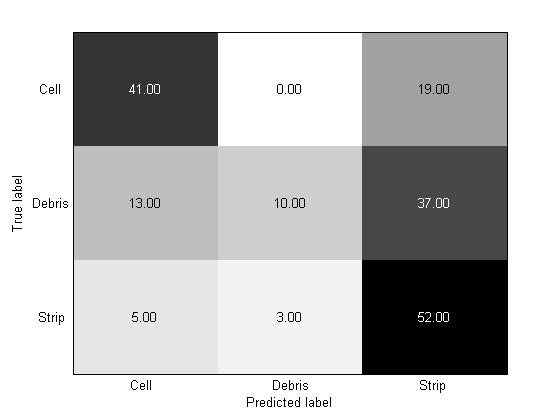
\includegraphics[width=\textwidth]{confusion_matrix/fig3_3_b.jpg}
    \caption{}
  \end{subfigure}
  \begin{subfigure}[b]{0.3\textwidth}
    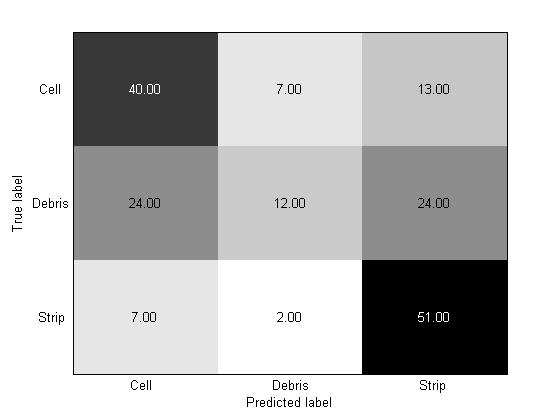
\includegraphics[width=\textwidth]{confusion_matrix/fig3_3_c.jpg}
    \caption{}
  \end{subfigure}
  \begin{subfigure}[b]{0.3\textwidth}
    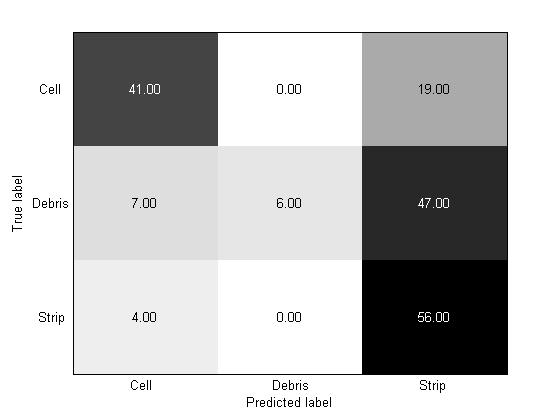
\includegraphics[width=\textwidth]{confusion_matrix/fig3_3_d.jpg}
    \caption{}
  \end{subfigure}
  \begin{subfigure}[b]{0.3\textwidth}
    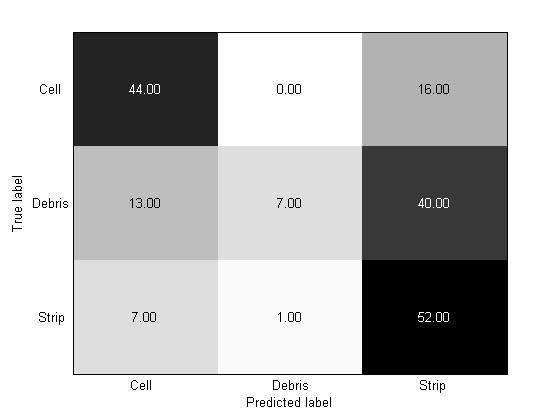
\includegraphics[width=\textwidth]{confusion_matrix/fig3_3_e.jpg}
    \caption{}
  \end{subfigure}
  \begin{subfigure}[b]{0.3\textwidth}
    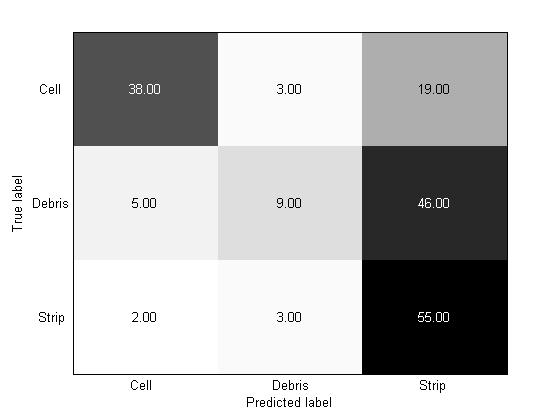
\includegraphics[width=\textwidth]{confusion_matrix/fig3_3_f.jpg}
    \caption{}
  \end{subfigure}
  \caption{Confusion matrix of the SVM classifier trained on data with two feature parameters}
\end{figure}
Based on the result in Table 3.4, we achieve the accuracy of the SVM classifier trained on the data with three feature parameters shown in Table 3.5. All the combination as Table 3.5 shown are evolved from the significant four combination shown in Table 3.4 by adding new feature parameter selected from the remaining feature parameters. 
\begin{table}[!h]
\begin{center}
\renewcommand{\arraystretch}{0.5}
\begin{tabular}{|| c | c c ||}
\hline
 Feature Combination & p-ENT\;p-CON\&s-CLS & p-ENT\;p-CON\&s-CLP  \\
 \hline
 Accuracy & 60.56\% & 60.00\% \\
 \hline
 Confusion Matrix & Figure 3.4(a) & Figure 3.4(b)  \\
 \hline
 \hline
 Feature Combination & p-ASM\;p-CON\&s-CLP & p-SEN\;p-CON\&s-CLP \\
 \hline
 Accuracy & 59.44\% & 60.56\% \\
 \hline
 Confusion Matrix & Figure 3.4(c) & Figure 3.4(d)  \\
 \hline
 \hline
  Feature Combination & p-MAP\;p-CON\&s-VAR & p-MAP\;p-CON\&s-SEN \\
 \hline
 Accuracy & 60.00\% & 60.56\% \\
 \hline
 Confusion Matrix & Figure 3.4(e) & Figure 3.4(f)  \\
 \hline
\end{tabular}
\end{center}
\caption{The accuracy of SVM classifier trained on 360 data with three feature parameters}
\end{table}
\begin{figure}[!h]
\centering
  \begin{subfigure}[b]{0.3\textwidth}
    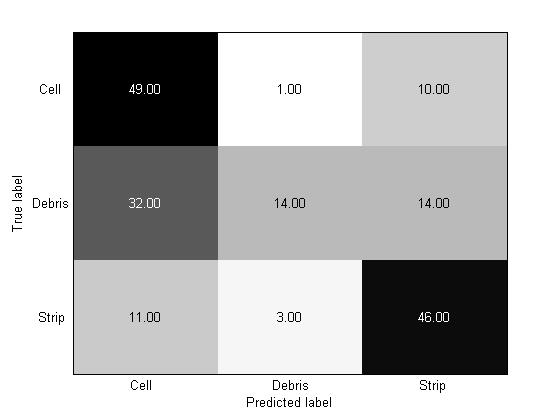
\includegraphics[width=\textwidth]{confusion_matrix/fig3_4_a.jpg}
    \caption{}
  \end{subfigure}
  \begin{subfigure}[b]{0.3\textwidth}
    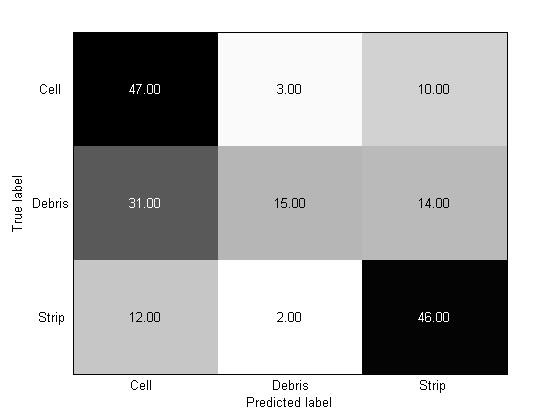
\includegraphics[width=\textwidth]{confusion_matrix/fig3_4_b.jpg}
    \caption{}
  \end{subfigure}
  \begin{subfigure}[b]{0.3\textwidth}
    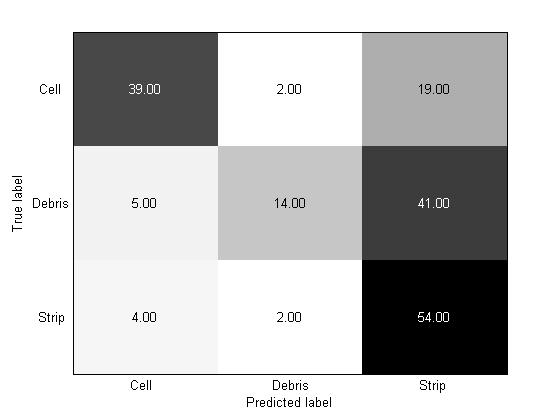
\includegraphics[width=\textwidth]{confusion_matrix/fig3_4_c.jpg}
    \caption{}
  \end{subfigure}
  \begin{subfigure}[b]{0.3\textwidth}
    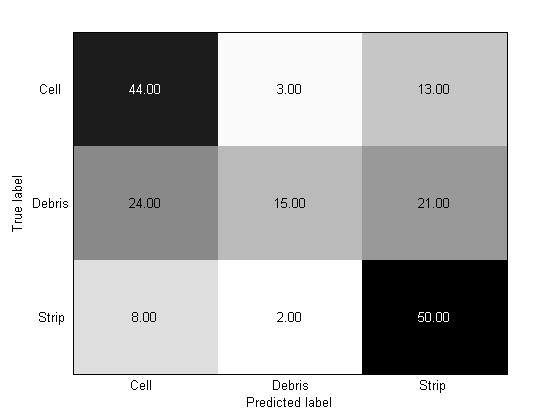
\includegraphics[width=\textwidth]{confusion_matrix/fig3_4_d.jpg}
    \caption{}
  \end{subfigure}
  \begin{subfigure}[b]{0.3\textwidth}
    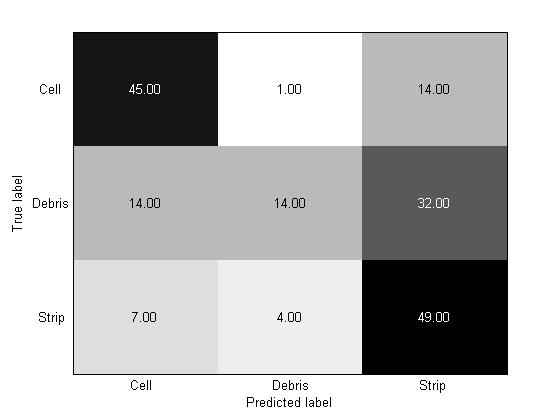
\includegraphics[width=\textwidth]{confusion_matrix/fig3_4_e.jpg}
    \caption{}
  \end{subfigure}
  \begin{subfigure}[b]{0.3\textwidth}
    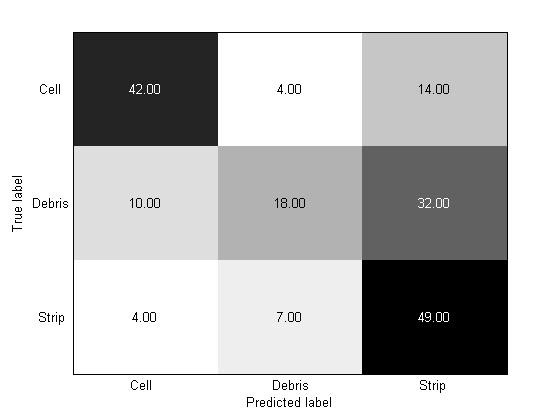
\includegraphics[width=\textwidth]{confusion_matrix/fig3_4_f.jpg}
    \caption{}
  \end{subfigure}
  \caption{Confusion matrix of the SVM classifier trained on data with three feature parameters}
\end{figure}
The confusion matrix presents the visualization of a classifier's performance. We can see from the Figure 3.3 that the classifier has trouble in distinguishing the type between cell and debris using feature p-ENT and p-CON and the type between debris and strip using the rest combination in Table 3.4. By comparing the confusion matrix between Figure 3.3 and Figure 3.4, adding new feature parameter mitigates the trouble.   
\begin{table}[!h]
\begin{center}
\renewcommand{\arraystretch}{0.7}
\begin{tabular}{|| c | c ||}
\hline
 Feature Combination & Accuracy  \\
\hline
 p-ENT\;p-CON\;s-CLS\&s-COR & 61.11\% \\
 p-ENT\;p-CON\;s-CLP\&s-COR & 61.11\% \\
 p-SEN\;p-CON\;s-CLP\&p-SAV & 61.67\% \\
 p-SEN\;p-CON\;s-CLP\&p-MEA & 61.67\% \\
 p-MAP\;p-CON\;s-VAR\&p-SAV & 61.67\% \\
 p-MAP\;p-CON\;s-VAR\&p-MEA & 61.67\% \\
\hline
\end{tabular}
\end{center}
\caption{The accuracy of SVM classifier trained on 360 data with four feature parameters}
\end{table}
Table 3.6 indicate that the highest accuracy increases from 60.56\% to 61.67\% by adding a new feature. For example, the texture feature p-SVA is added into the combination including s-CLP, p-CON and p-SEN. In addition, we can find a situation that adding either s-CLS or s-CLP can result in the same accuracy as well as adding either p-SAV or p-MEA. We introduce the line chart of these four texture features as Figure 3.5 shown. 
\begin{figure}[!h]
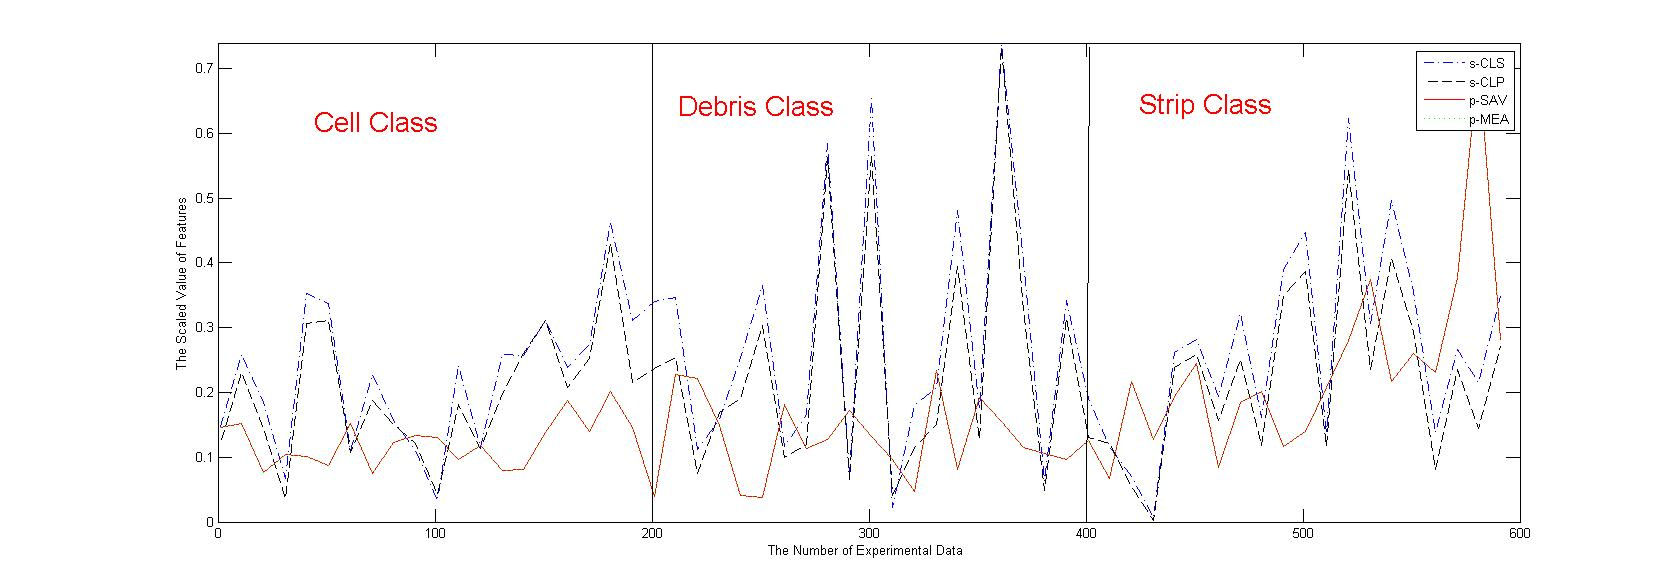
\includegraphics[width=\linewidth]{fig3_5}
\caption{The line chart for four texture features}
\end{figure}
In the figure, we can obviously see the correlation between two texture features. Especially, the feature p-SAV and p-MEA have the same values after scaling. Thus, adding feature p-SAV or p-MEA makes no difference in increasing the accuracy of the classifier. However, the feature s-CLS and s-CLP may have the different result after adding one of them. Table 3.7 shows the accuracy of  experimental data with five feature parameters. 
\begin{table}[!h]
\begin{center}
\renewcommand{\arraystretch}{0.7}
\begin{tabular}{|| c | c ||}
\hline
 Feature Combination & Accuracy  \\
\hline
 p-ENT\;p-CON\;s-CLS\;s-COR\&p-DIS & 62.22\% \\
 p-ENT\;p-CON\;s-CLP\;s-COR\&p-DIS & 59.44\% \\
 p-SEN\;p-CON\;s-CLP\;p-SAV\&s-COR & 61.67\% \\
 p-SEN\;p-CON\;s-CLP\;p-MEA\&s-COR & 61.67\% \\
 p-MAP\;p-CON\;s-VAR\;p-SAV\&p-SVA & 62.78\% \\
\hline
\end{tabular}
\end{center}
\caption{The accuracy of SVM classifier trained on 360 data with five feature parameters}
\end{table}
As Table 3.7 presented, by adding feature p-DIS, the combination with feature s-CLS results in the increased accuracy, while the combination with feature s-CLP results in the decreased accuracy. This result indicates that although feature s-CLS and s-CLP are correlated, they can be affected by another feature. On the contrary, the third row and fourth row results denote that feature p-SAV and p-MEA are not affected by adding new feature because they are considered as one feature after scaling. Currently, the highest accuracy of the SVM classifier trained on the data with the feature combination including p-MAP, p-CON, s-VAR, p-SAV and p-SVA is 62.78\%. When adding one more feature into this combination, the accuracy decreases to 62.22\%. Nevertheless, the combination including p-ENT, p-CON, s-CLS, s-COR and p-DIS results in the higher accuracy by adding feature p-SEN as Table 3.8 shown.
\begin{table}[!h]
\begin{center}
\renewcommand{\arraystretch}{0.7}
\begin{tabular}{|| c | c ||}
\hline
 Feature Combination & Accuracy  \\
\hline
 Six Features &\\
\hline
 p-ENT\;p-CON\;s-CLS\;s-COR\;p-DIS\&p-SEN & 63.33\% \\
 p-MAP\;p-CON\;s-VAR\;p-SAV\;p-SVA\&p-DIS & 62.22\% \\
\hline
 Seven Features & \\
\hline
 p-ENT\;p-CON\;s-CLS\;s-COR\;p-DIS\;p-SEN\&p-VAR & 63.89\% \\
 \hline
 Eight Features & \\
\hline
 p-ENT\;p-CON\;s-CLS\;s-COR\;p-DIS\;p-SEN\;p-VAR\&p-CLP & 63.89\% \\
  \hline
 Nine Features & \\
\hline
 p-ENT\;p-CON\;s-CLS\;s-COR\;p-DIS\;p-SEN\;p-VAR\;p-CLP\&p-SVA & 62.78\% \\
\hline
\end{tabular}
\end{center}
\caption{The accuracy of SVM classifier trained on 360 data with more than five feature parameters}
\end{table}
After continuing adding feature p-VAR, the accuracy of the SVM classifier reaches the peak because adding more features can't result in accuracy increasing. Instead, when adding the feature p-SVA, the accuracy commences decreasing as Table 3.8 shown. In the meanwhile, a line chart in Figure 3.6 is created to conclude the results at each step. 
\begin{figure}[!h]
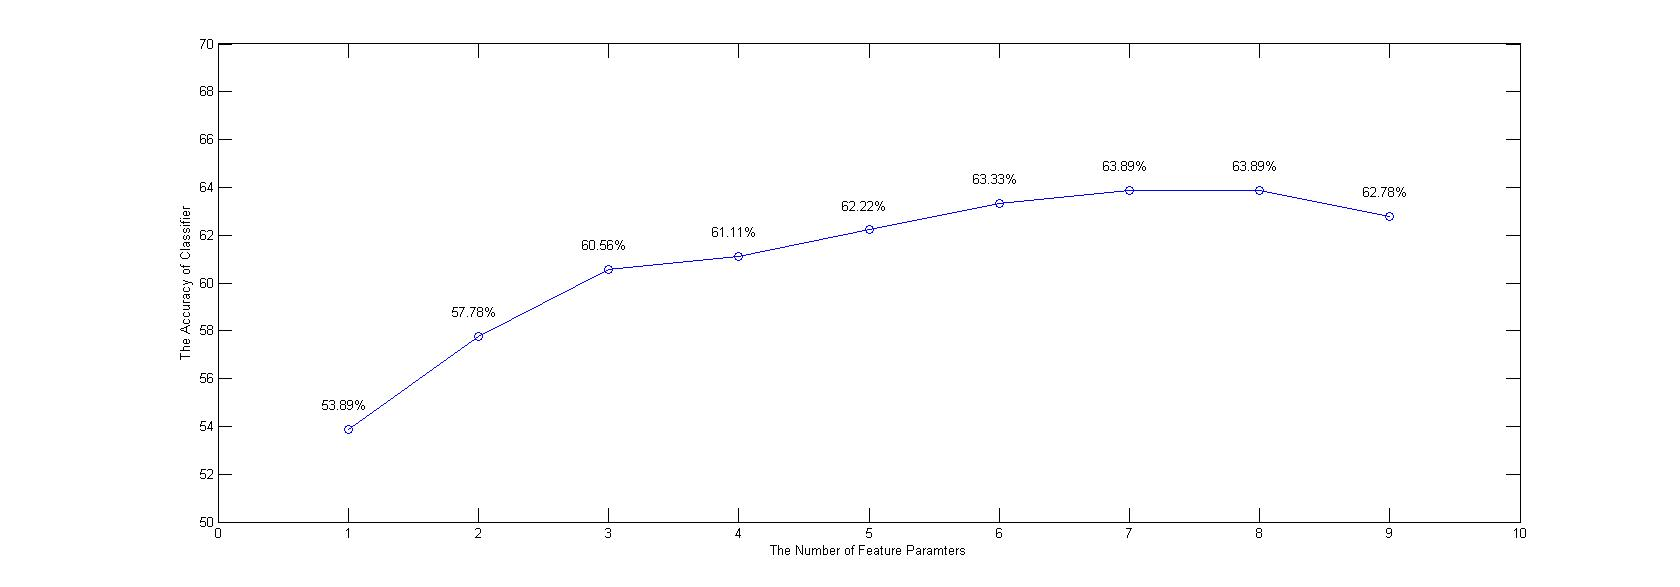
\includegraphics[width=\linewidth]{fig3_6}
\caption{One scenario of selecting feature parameters using forward propagation approach (600 experimental data)}
\end{figure}
Therefore, we get the highest accuracy 63.89\% by using the feature combination consisting of s-COR, s-CLS, p-CON, p-ENT, p-DIS, p-SEN and p-VAR. By applying this approach, we select eight texture features, and achieve the suitable SVM classifier with the highest accuracy by using these selected feature parameters.\par
In real situation, even though we achieve the classifier with the highest accuracy, it sometimes can't generalize to new examples. This is called classifier overfitting which describes the situation that the the classifier fits training set very well. In other words, the SVM classifier is overly optimistic. Thus, validating the classifier is necessary. We extracted 20 data examples from each class, and a validating data set is constructed with total 60 data examples. By adding these data examples into training data set, the accuracy of the classifier decreases from 63.89\% to 41.11\%. The result reveals the fact that the previous classifier is overfitted with the specific feature parameter combination. To further examine, we apply a common method called k-folder cross-validation in the training data set. Through specifying the parameter k with the value 5, we achieve the result for each folder as Table 3.9 shown.  
\begin{table}[!h]
\begin{center}
\begin{tabular}{||c c | c c ||}
\hline
Subset Index & Accuracy & Subset Index & Accuracy \\[0.7ex]
\hline\hline
1 & 43.06\% & 4 & 44.44\% \\
2 & 47.22\% & 5 & 51.39\% \\
3 & 45.83\% &  &  \\
\hline
 & & Average & 46.39\% \\
\hline
\end{tabular}
\caption {5-folder cross-validation result of SVM classifier}
\end{center}
\end{table}
From the table, we can see the average accuracy is 46.39\% which is far away from the highest accuracy 63.89\%. As a result, the validation process confirm the fact that the SVM classifier achieved from previous experiment is neither stable nor general. \par
The previous experiment and classifier validation process reveal the problem that the SVM classifier with the accuracy 63.89\% fit the training data set too well to generalize to new examples. Once new examples added, the classifier can not keep the accuracy anymore. To solve, we involve more training data to improve the generalization of the classifier. At this time, we apply all 3000 experimental data. Within the 3000 data, there are 957 data labeled as Cell, 1555 data labeled as Debris and 488 data labeled as Strip. To construct the training data set, we select 1200 out of 3000 experimental data. Also, we select 600 out of 3000 data as the testing data set and the rest as the validating data set. Then, by repeating the experiment with the new experimental data, we achieve the each accuracy of the SVM classifier trained on the data with single feature as Table 3.10 shown. 
\begin{table}[!h]
\begin{center}
\renewcommand{\arraystretch}{0.5}
\begin{tabular}{||c c c c c c ||}
\hline
Index & Feature & Accuracy & Index & Feature & Accuracy \\[0.7ex]
\hline\hline
1 & s-ASM & 53.33\% & 21 & p-ASM & 56.50\% \\
2 & s-CON & 53.33\% & 22 & p-CON & 53.33\% \\
3 & s-COR & 53.33\% & 23 & p-COR & 53.33\% \\
4 & s-VAR & 53.33\% & 24 & p-VAR & 53.33\% \\
5 & s-IDM & 53.33\% & 25 & p-IDM & 53.33\% \\
6 & s-SAV & 53.33\% & 26 & p-SAV & 53.33\% \\
7 & s-SEN & 53.33\% & 27 & p-SEN & 53.33\% \\
8 & s-SVA & 53.33\% & 28 & p-SVA & 53.33\% \\
9 & s-ENT & 53.33\% & 29 & p-ENT & 55.67\% \\
10 & s-DEN & 53.33\% & 30 & p-DEN & 53.33\% \\
11 & s-DVA & 53.33\% & 31 & p-DVA & 53.33\% \\
12 & s-DIS & 53.33\% & 32 & p-DIS & 53.33\% \\
13 & s-CLS & 53.33\% & 33 & p-CLS & 53.33\% \\
14 & s-CLP & 53.33\% & 34 & p-CLP & 53.33\% \\
16 & s-MAP & 53.33\% & 36 & p-MAP & 55.50\% \\
17 & s-MEA & 53.33\% & 37 & p-MEA & 53.33\% \\
\hline
\end{tabular}
\caption {The accuracy of the SVM classifier trained on 1200 experimental data with single feature parameter}
\end{center}
\end{table}
From the Table 3.10 we can see only using feature p-ASM, p-ENT, and p-MAP for classification can achieve the accuracy that is more than 53.33\%. Since there are 320 debris data in testing data set, the accuracy 53.33\% has the same meaning with the accuracy 33.33\%. Based on the three features, we select one more feature to evolve the combination with two feature parameters and list six results with high accuracy in Table 3.11.
\begin{table}[!h]
\begin{center}
\renewcommand{\arraystretch}{0.5}
\begin{tabular}{|| c | c c c ||}
\hline
 Feature Combination& p-CON\&p-MAP & p-ASM\&p-CON & p-ENT\&p-DIS \\
 \hline
 Accuracy & 58.33\% & 58.00\% & 58.00\% \\
 \hline
 \hline
 Feature Combination& p-CON\&p-ENT & s-SAV\&p-ASM & p-ASM\&p-SAV \\
 \hline
 Accuracy & 57.83\% & 57.17\% & 57.17\% \\
 \hline
\end{tabular}
\end{center}
\caption{The accuracy of SVM classifier trained on 1200 data with two feature parameters}
\end{table}
The result in Table 3.11 indicates the accuracy increases by adding another feature parameter. In general, each feature parameter in the same combination is from different group. For instance, the feature p-CON comes from group 1 which is the measures of Contrast, while the feature p-MAP comes from group 2 which is the measures of Uniformity or Orderliness of pixels. For each combination in Table 3.11, we add one more feature parameter and achieve higher accuracy shown in Table 3.12. 
\begin{table}[!h]
\begin{center}
\renewcommand{\arraystretch}{0.5}
\begin{tabular}{|| c | c c ||}
\hline
 Feature Combination & p-CON\;p-MAP\&p-COR & p-ASM\;p-CON\&p-SEN  \\
 \hline
 Accuracy & 59.67\% & 58.50\% \\
 \hline
 \hline
 Feature Combination & p-ENT\;p-DIS\&s-SAV & p-CON\;p-ENT\&s-SAV \\
 \hline
 Accuracy & 59.33\% & 59.67\% \\
 \hline
 \hline
  Feature Combination & s-SAV\;p-ASM\&p-CON & p-ASM\;p-SAV\&p-CON \\
 \hline
 Accuracy & 58.00\% & 57.83\% \\
 \hline
\end{tabular}
\end{center}
\caption{The accuracy of SVM classifier trained on 1200 data with three feature parameters}
\end{table}
For most combinations containing three feature parameters, each feature comes from different group as we mentioned for the combination with two feature parameters. By adding one more feature into the combination, we achieve the result shown in Table 3.13. 
\begin{table}[!h]
\begin{center}
\renewcommand{\arraystretch}{0.7}
\begin{tabular}{|| c | c ||}
\hline
 Feature Combination & Accuracy  \\
\hline
 p-CON\;p-MAP\;p-COR\&s-MAP & 60.17\% \\
 p-ASM\;p-CON\;p-SEN\&s-ASM & 58.83\% \\
 p-ENT\;p-DIS\;s-SAV\&s-MEA & 59.67\% \\
 p-CON\;p-ENT\;s-SAV\&s-MEA & 60.67\% \\
 s-SAV\;p-ASM\;p-CON\&p-ENT & 59.17\% \\
 p-ASM\;p-SAV\;p-CON\&p-SEN & 58.67\% \\
\hline
\end{tabular}
\end{center}
\caption{The accuracy of SVM classifier trained on 1200 data with four feature parameters}
\end{table}
For each combination in Table 3.12, the accuracy increases through adding new feature parameter. When the number of feature parameters is five, the accuracy is increasing as well shown in Table 3.14.
\begin{table}[!h]
\begin{center}
\renewcommand{\arraystretch}{0.7}
\begin{tabular}{|| c | c ||}
\hline
 Feature Combination & Accuracy  \\
\hline
 p-CON\;p-MAP\;p-COR\;s-MAP\&s-SEN & 60.33\% \\
 p-ASM\;p-CON\;p-SEN\;s-ASM\&s-SAV & 59.67\% \\
 p-ENT\;p-DIS\;s-SAV\;s-MEA\&s-ASM & 60.67\% \\
 p-CON\;p-ENT\;s-SAV\;s-MEA\&s-MAP & 60.83\% \\
 s-SAV\;p-ASM\;p-CON\;p-ENT\&s-IDM & 59.83\% \\
 p-ASM\;p-SAV\;p-CON\;p-SEN\&s-VAR & 59.17\% \\
\hline
\end{tabular}
\end{center}
\caption{The accuracy of SVM classifier trained on 1200 data with five feature parameters}
\end{table}
However, when the number of feature parameters reaches six, the SVM classifier can't be improved by using some feature parameter combinations. For example, the SVM classifier with accuracy 59.67\% no longer increases when adding feature s-SAV. Nevertheless, when adding feature s-SVA, the accuracy decreases. Considering this situation, we eliminate the classifiers with accuracy below 60\%.   
\begin{table}[!b]
\begin{center}
\renewcommand{\arraystretch}{0.7}
\begin{tabular}{|| c | c ||}
\hline
 Feature Combination & Accuracy  \\
\hline
 Six Features &\\
\hline
 p-CON\;p-MAP\;p-COR\;s-MAP\;s-SEN\&s-DIS & 60.67\% \\
 p-ENT\;p-DIS\;s-SAV\;s-MEA\;s-ASM\&s-MAP & 61.17\% \\
 p-CON\;p-ENT\;s-SAV\;s-MEA\;s-MAP\&p-SVA & 61.33\% \\
\hline
 Seven Features & \\
\hline
 p-CON\;p-MAP\;p-COR\;s-MAP\;s-SEN\;s-DIS\&s-CON & 60.67\% \\
 p-ENT\;p-DIS\;s-SAV\;s-MEA\;s-ASM\:s-MAP\&s-IDM & 61.50\% \\
 p-CON\;p-ENT\;s-SAV\;s-MEA\;s-MAP\;p-SVA\&s-CON & 61.33\% \\
 \hline
 Eight Features & \\
\hline
 p-CON\;p-MAP\;p-COR\;s-MAP\;s-SEN\;s-DIS\;s-CON\&p-SAV & 60.83\% \\
 p-ENT\;p-DIS\;s-SAV\;s-MEA\;s-ASM\:s-MAP\;s-IDM\&p-CLS & 61.50\% \\
 p-CON\;p-ENT\;s-SAV\;s-MEA\;s-MAP\;p-SVA\;s-CON\&s-SEN & 61.33\% \\
\hline
 Nine Features & \\
\hline
  p-ENT\;p-DIS\;s-SAV\;s-MEA\;s-ASM &\\
  s-MAP\;s-IDM\;p-CLS\&s-DVA & 61.50\% \\
\hline
 Eleven Features & \\
\hline
 p-ENT\;p-DIS\;s-SAV\;s-MEA\;s-ASM &\\
 s-MAP\;s-IDM\;p-CLS\;s-DVA\;s-COR\&p-CLP & 61.67\% \\
\hline
 Twelve Features & \\
\hline
 p-ENT\;p-DIS\;s-SAV\;s-MEA\;s-ASM\;s-MAP &\\
 s-IDM\;p-CLS\;s-DVA\;s-COR\;p-CLP\&s-CLP & 61.33\% \\
\hline
\end{tabular}
\end{center}
\caption{The accuracy of SVM classifier trained on 1200 data with more than five feature parameters}
\end{table}
Thus, we have three SVM models left. With the number of feature parameters increased, two classifiers reveal the fact that the accuracy can't grow. By adding two more feature parameters, the accuracy is still the same. Therefore, there is only one feature parameter combination remained. Eventually, the SVM classifier reaches the highest accuracy 61.67\% when it is trained on the data with 11 feature parameters which are s-ASM, s-COR, s-IDM, s-SAV, s-DVA, s-MAP, s-MEA, p-ENT, p-DIS, p-CLS and p-CLP. By adding the validating data set into training data set, the accuracy of the selected model decreases 0.34\%. The slight change is acceptable since the experimental data we used are not ideal. Figure 3.7 presents a scenario that the accuracy variation of  the SVM classifier with the number of feature parameters increases for this combination.
\begin{figure}
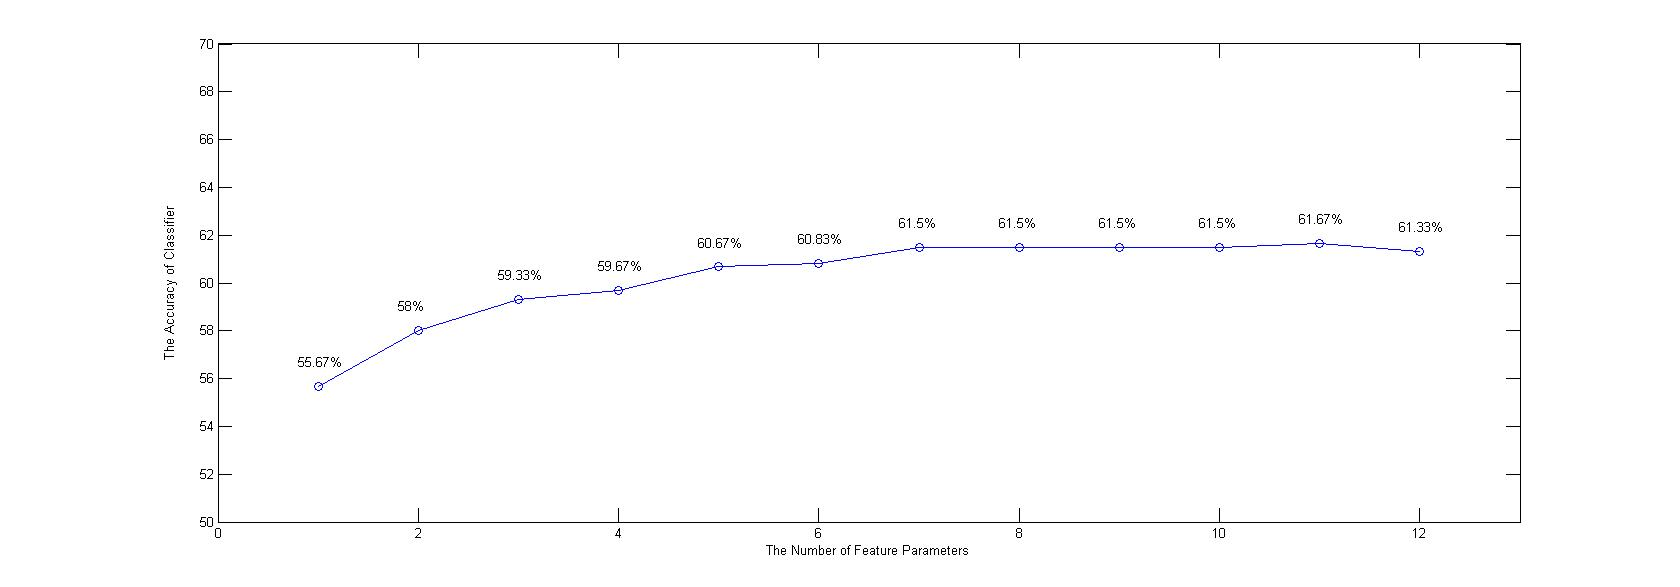
\includegraphics[width=\linewidth]{fig3_7}
\caption{One scenario of selecting feature parameters using forward propagation approach (3000 experimental data)}
\end{figure}
The primary goal of selecting feature parameters is to prevent invalid texture feature from affecting the accuracy of classification. Thus, the classifier trained on the data with all feature parameters should have lower accuracy than the one selected from the previous experiment. Through forward propagation approach, we achieve the highest accuracy of the SVM classifier is 61.67\% by using 11 feature parameters. However, when training the SVM classifier with all 32 feature parameters, we attain a higher accuracy 64.17\%. Obviously, the previous experimental approach fails to reach the goal. To improve, another feature selection approach is proposed. In contrast to adding feature parameter, we monitor the change of the SVM classifier's accuracy by directly removing invalid feature parameter from the original combination containing all 32 feature parameters. Firstly, we monitor the variations of each accuracy when removing a feature parameter. the accuracy is increased when the feature s-CON, p-ASM, p-ENT or p-MAP is removed from the combination shown in Table 3.16. 
\begin{table}[!h]
\begin{center}
\renewcommand{\arraystretch}{0.5}
\begin{tabular}{|| c | c | c c c||}
\hline
 Feature Removed & NONE & s-CON & p-ASM & p-MAP  \\
 \hline
 Accuracy & 64.17\% & 64.67\% & 65.00\% & 65.17\% \\
 \hline
\end{tabular}
\end{center}
\caption{The accuracy change of SVM classifier after removing a feature parameter from experimental data}
\end{table}
By comparing with Table 3.10, we achieve a totally conflicting result. For previous experimental approach, the new feature parameter combination is always created due to the old combination with high accuracy of SVM classifier. Thus, the feature p-ASM, p-ENT and p-MAP are considered as the first feature parameters that are selected. However, current experimental approach proves that these three feature parameters are considered as invalid features so that they may result in the lower accuracy of a classifier. After removing the feature p-MAP, we repeat the same process. The accuracy of the SVM classifier increases to 65.33\% by removing s-CON, s-SEN or s-MAP shown in Table 3.17.
\begin{table}[!h]
\begin{center}
\renewcommand{\arraystretch}{0.5}
\begin{tabular}{|| c | c | c c ||}
\hline
 Feature Removed & p-MAP & p-MAP\&s-CON & p-MAP\&p-SVA \\
 \hline
 Accuracy & 65.17\% & 65.33\% & 65.33\% \\
 \hline
\end{tabular}
\end{center}
\caption{The accuracy change of SVM classifier after removing two feature parameters from experimental data}
\end{table}
Since the SVM classifier can reach the same accuracy by removing the feature s-CON or p-SVA, we examine separately for each feature parameter. Due to the combination removing the feature s-CON, the accuracy of the classifier increases to 65.50\% after the feature parameter s-COR, p-VAR or p-CLS is removed shown in Table 3.18. 
\begin{table}[!h]
\begin{center}
\renewcommand{\arraystretch}{0.5}
\begin{tabular}{|| c | c | c c c||}
\hline
 & Features Have Removed & & Feature Is Removed &\\
\hline
 Feature & p-MAP\&s-CON & s-COR & p-VAR & p-CLS\\
 \hline
 Accuracy & 65.33\% & 65.50\% & 65.50\% & 65.50\% \\
 \hline
 Feature & p-MAP\&p-SVA & & s-CON &\\
 \hline
 Accuracy & 65.33\% & & 65.17\% & \\
 \hline
\end{tabular}
\end{center}
\caption{The accuracy change of SVM classifier after removing three feature parameters from experimental data}
\end{table}
In addition, Table 3.18 presents another result that after removing feature p-SVA, the accuracy commences decreasing. Therefore, we start the first scenario from removing the feature s-COR.    
\begin{table}[!h]
\begin{center}
\renewcommand{\arraystretch}{0.5}
\begin{tabular}{|| c | c | c | c | c | c ||}
\hline
 Step & Feature & Accuracy & Step & Feature & Accuracy \\
\hline
 0 & p-MAP\;\&\;s-CON & 65.33\% & & & \\
\hline
 1 & s-COR & 65.50\% & 6 & p-DEN & 65.33\% \\
 2 & p-SVA & 65.50\% & 7 & s-CLS & 65.33\% \\
 3 & p-ASM & 65.50\% & 8 & s-CLP & 65.50\% \\
 4 & s-ENT & 65.50\% & 9 & s-SVA & 65.50\% \\
 5 & p-CLP & 65.50\% & 10 & p-VAR & 65.17\% \\
\hline
\end{tabular}
\end{center}
\caption{The first scenario of selecting a SVM classifier starting with removing feature s-COR}
\end{table}
However, by sequentially removing feature p-SVA, p-ASM, s-ENT, p-CLP, the highest accuracy is still 65.50\%. When removing feature p-DEN, the accuracy decreases. Even though the accuracy is back to 65.50\% by keeping removing feature s-CLP, it decrease significantly by removing feature p-VAR. Thus, we are unable to reach a higher accuracy by following the first scenario of selecting feature parameters for classification. 
We follow the same procedure and start examining the second scenario of selecting feature parameters shown in Table 3.20.
\begin{table}[!h]
\begin{center}
\renewcommand{\arraystretch}{0.5}
\begin{tabular}{|| c | c | c | c | c | c ||}
\hline
 Step & Feature & Accuracy & Step & Feature & Accuracy \\
\hline
 0 & p-MAP\;\&\;s-CON & 65.33\% & & & \\
\hline
 1 & p-VAR & 65.33\% & 4 & s-CLP & 65.50\% \\
 2 & p-CLS & 65.67\% & 5 & p-CLP & 65.17\% \\
 3 & p-SVA & 65.50\% &  &  & \\
\hline
\end{tabular}
\end{center}
\caption{The second scenario of selecting a SVM classifier starting with removing feature p-VAR}
\end{table}
The second scenario is simply. The accuracy reaches the peak when sequentially removing p-VAR and p-CLS. It decreases when removing more feature parameters. The third scenario of selecting feature parameters starts with removing feature p-CLS shown in Table 3.21. 
\begin{table}[!h]
\begin{center}
\renewcommand{\arraystretch}{0.5}
\begin{tabular}{|| c | c | c | c | c | c ||}
\hline
 Step & Feature & Accuracy & Step & Feature & Accuracy \\
\hline
 0 & p-MAP\;\&\;s-CON & 65.33\% & & & \\
\hline
 1 & p-CLS & 65.50\% & 6 & s-CLS & 65.50\% \\
 2 & p-SVA & 65.67\% & 7 & p-ASM & 65.50\% \\
 3 & s-CLP & 65.67\% & 8 & s-ASM & 65.50\% \\
 4 & p-CLP & 65.50\% & 9 & s-SEN & 65.33\% \\
 5 & s-COR & 65.67\% & & &  \\
\hline
\end{tabular}
\end{center}
\caption{The third scenario of selecting a SVM classifier starting with removing feature p-CLS}
\end{table}
It is more complex than the second scenario. We can select three feature combinations from it. Figure 3.8 presents a line chart to visualize the accuracy variation of the third scenario.
\begin{figure}
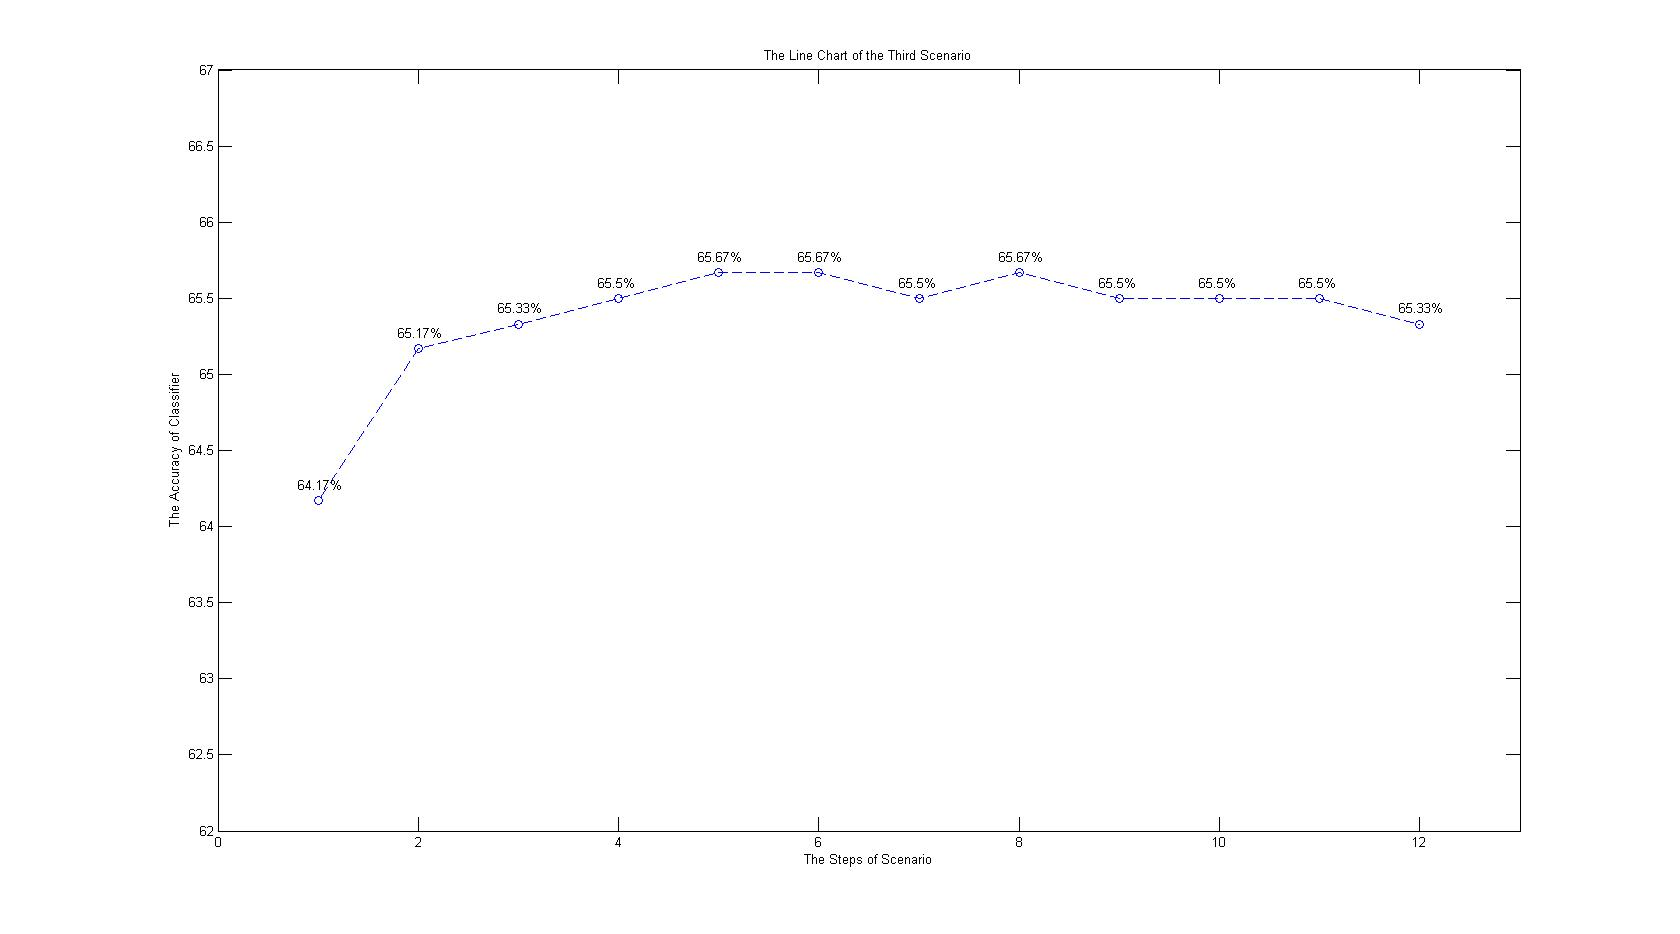
\includegraphics[width=\linewidth]{fig3_8c}
\caption{One scenario of selecting feature parameters using backward propagation approach}
\end{figure}
We create four SVM classifiers using the feature parameter combinations from second and third scenario shown in Table 3.22. 
\begin{table}[!h]
\begin{center}
\renewcommand{\arraystretch}{0.8}
\begin{tabular}{|| c | c | c | c | c ||}
\hline
 Classifier & Classifier & Number of & Accuracy & Accuracy \\
 Index & From Scenario &  Features & Before Validation & After Validation \\
\hline
 1 & 2 &28 & 65.67\% & 65.67\% \\
 2 & 3 &28 & 65.67\% & 65.50\% \\
 3 & 3 &27 & 65.67\% & 65.50\% \\
 4 & 3 &25 & 65.67\% & 65.50\% \\
\hline 
\end{tabular}
\end{center}
\caption{The comparison among four classifiers}
\end{table}
The table illustrates the basic information for the classifier using four selected feature combination for classification. The first classifier is created using the combination selected from the second scenario and the rest classifiers are created using the combinations from the third scenario. To select the best feature parameter combination, we perform the validation by adding validating data set in training data set for each classifier. As Table 3.22 shown, the classifier trained on data with feature combination selected from second scenario is the best. In addition, we apply the 10-folder cross-validation method in the first classifier. The result is shown in Table 3.23. 
\begin{table}[!h]
\begin{center}
\begin{tabular}{||c c | c c ||}
\hline
Subset Index & Accuracy & Subset Index & Accuracy \\[0.7ex]
\hline\hline
1 & 70.50\% & 6 & 70.50\% \\
2 & 65.50\% & 7 & 64.00\% \\
3 & 67.50\% & 8 & 60.00\% \\
4 & 65.50\% & 9 & 62.50\% \\
5 & 65.00\% & 10 & 67.00\%  \\
\hline
 & & Average & 65.80\% \\
\hline
\end{tabular}
\caption {10-folder cross-validation result of SVM classifier}
\end{center}
\end{table}
The average accuracy of the cross-validation further confirm the classifier we selected is satisfied with our expectation. 
\subsection{The SVM Kernel Optimization}
In this research, we apply the RBF kernel which has two important parameters C and $\gamma$. Practically speaking, a SVM classifier can be further optimized by identifying the best parameter pair of (C, $\gamma$). We estimate the parameter pair of (C, $\gamma$) to C = $2^0$ and $\gamma = 0.07$ as the default values and achieve the SVM classifier with accuracy 65.67\%. Then, we try all combinations between parameter C from $2^{-5}$ to $2^{15}$ and $\gamma$ from $2^{-15}$ to $2^3$ (for example, C = $2^{-5}$, $2^{-4}$, $\ldots$, $2^{15}$, $\gamma$ = $2^{-15}$, $2^{-14}$, $\ldots$, $2^3$) to identify the best parameter pair. We list some of the result in Table 3.24. 
\begin{table}[!h]
\begin{center}
\renewcommand{\arraystretch}{0.8}
\begin{tabular}{||c| c c c c c c c c c ||}
\hline
 \backslashbox{C}{$\gamma$} & $2^{-15}$ & $2^{-14}$ & $\ldots$ & $2^{-3}$ & $2^{-2}$ & $2^{-1}$ & $\ldots$ & $2^2$ & $2^3$ \\
\hline
 $2^{-5}$ & 53.33 & 53.33 & $\ldots$ & 53.33 & 56.67 & 58.50 & $\ldots$ & 65.33 & 59.33 \\
 $2^{-4}$ & 53.33 & 53.33 & $\ldots$ & 57.00 & 58.67 & 62.17 & $\ldots$ 
& 69.00 & 68.67 \\
 $\ldots$ & $\ldots$ & $\ldots$ & $\ldots$ & $\ldots$ & $\ldots$ & $\ldots$ & $\ldots$ 
& $\ldots$ & $\ldots$ \\
 $2^{9}$ & 58.16 & 59.00 & $\ldots$ & 78.33 & 79.67 & \cellcolor{blue!25}80.00 & $\ldots$ 
& 66.00 & 67.67 \\
 $\ldots$ & $\ldots$ & $\ldots$ & $\ldots$ & $\ldots$ & $\ldots$ & $\ldots$ & $\ldots$ 
& $\ldots$ & $\ldots$ \\
 $2^{12}$ & 63.00 & 64.83 & $\ldots$ & \cellcolor{blue!25}80.33 & 79.50 & 75.50 & $\ldots$ 
& 65.83 & 67.67 \\
 $\ldots$ & $\ldots$ & $\ldots$ & $\ldots$ & $\ldots$ & $\ldots$ & $\ldots$ & $\ldots$ 
& $\ldots$ & $\ldots$ \\
 $2^{14}$ & 67.33 & 67.83 & $\ldots$ & 79.33 & 76.67 & 74.33 & $\ldots$ 
& 65.83 & 67.67 \\
 $2^{15}$ & 67.83 & 67.83 & $\ldots$ & 79.33 & 75.33 & 72.83 & $\ldots$ 
& 65.83 & 67.67 \\
\hline
\end{tabular}
\caption {The various pairs of (C, $\gamma$) values}
\end{center}
\end{table}
Based on the results, the accuracy of the SVM classifier is 80.33\% when C=$2^{12}$ and $\gamma = 2^{-3}$ and 80.00\% when C=$2^{9}$ and $\gamma = 2^{-1}$. By adding validating data set and the result is shown in Table 3.25. 
\begin{table}[!h]
\begin{center}
\renewcommand{\arraystretch}{0.8}
\begin{tabular}{|| c | c | c | c ||}
\hline
 Classifier Index & pair of (C, $\gamma$) & Accuracy & Accuracy \\
 & & Before Validation & After Validation \\
\hline
 1 & ($2^{9}$, $\gamma = 2^{-1}$) & 80.00\% & 78.83\% \\
 2 & ($2^{12}$, $\gamma = 2^{-3}$) & 80.33\% & 80.5\% \\
\hline 
\end{tabular}
\end{center}
\caption{The comparison between two pairs of (C, $\gamma$)}
\end{table}
The accuracy variation of the first classifier is larger than the second classifier. Therefore, we consider the first classifier has higher risk than the second one in failing to generalize to new examples. To conclude, we consider the second SVM classifier as the best experimental result and achieve the confusion matrix as Figure 3.9 shown. 
\begin{figure}[!b]
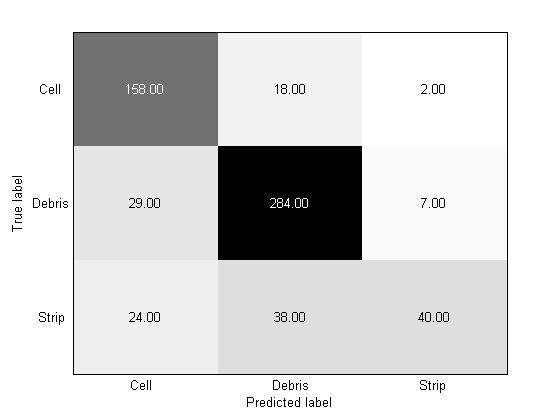
\includegraphics[width=\linewidth]{fig3_9}
\caption{The confusion matrix of the best SVM classifier}
\end{figure}
\section{Conclusion}
In this research, we have 3000 experimental data extracting from GLCM which is a statistic method to illustrate the image data. To prevent ambiguous images from increasing the error rate of a SVM classifier, we manually select 600 out of the 3000 experimental data for which we have high level confidence in pre-classification. By taking the forward propagation method for selecting feature parameters, we attain the SVM classifier with accuracy 63.89\%. However, through applying validating data set and the 5-folder cross validation methods, the SVM classifier using the selected feature combination as attribute parameters is proved neither stable nor being able to generalize to new examples. To make the SVM classifier more common to new examples, we increase the amount of experimental data and apply all 3000 experimental data for the forward propagation method. As a result, we achieve a new SVM classifier with accuracy 61.67\% which is lower than the previous achieved one. However, by taking the validation process, this classifier only have a slight change which is acceptable in reality. For the classifier using selected feature combination as attribute parameters, it contains 11 feature parameters. Nevertheless, when we test the SVM classifier trained on the same size of data with 32 texture feature as attribute parameters, we achieve a classifier with higher accuracy which is 64.17\%. The result reveals a fact that there are some feature parameters that also are able to improve the SVM classifier performance but we can't reach them by forward propagation approach. To solve, a new method of selecting feature parameters is proposed. Instead of adding feature parameter, we monitor the accuracy variation of a SVM classifier when eliminating an existing feature parameter. By applying the method, we achieve four feature combination resulting in the accuracy 65.67\%. Eventually, we select the classifier using the feature combination selected from the second scenario as attribute parameters because it is the only one whose accuracy doesn't change when adding the validating data set into the training data set. We also apply 10-folder cross-validation approach for further validation. The average accuracy of the cross-validation confirm the classifier we select doesn't have overfitting problem. Finally, by identifying the best pair of (C,$\gamma$), we choose the pair of ($2^{12}$,$2^{-3}$) and achieve the best SVM classifier with accuracy 80.33\% from the experiment. The confusion matrix also reveals that the selected SVM classifier has good performance in selecting diffraction image type between cell and debris but trouble in distinguishing image type between strip and debris. Nevertheless, since the debris and strip are considered as invalid image type, the trouble can be ignored.      
%Chapter 4

\renewcommand{\thechapter}{4}

\chapter{Summary}
This thesis research aims at automated classification of diffraction images based on their texture features. To achieve the goal, we wanted to develop and verify a tool for extracting texture feature from GLCM. We also wanted to validate whether the SVM can be applied for image classification by using texture features of diffraction images. In addition, we tried to use two diffraction images captured at the same time but from different directions to improve the configuration. Also, we wanted to utilize the SVM kernel method to improve the performance of the SVM classifier. This thesis research achieved all its objectives by performing the empirical study.\par
Through the empirical study, we performed a case study in selecting features by using the EFCS approach which was performed in Thati's research\cite{Thati}. Due to the results of the case study, we found the classification accuracy is 70.33\% by using six out of 17 feature parameters. By contrast, the classification accuracy is 80.33\% by using 28 out of 34 feature parameters in our experiment. The comparison indicates that using two diffraction images has higher performance in pattern recognition of diffraction image. \par
To extract texture features from GLCM, we developed an application in JAVA with simple but convenient UI. By performing functional testing for the newly developed application, we found bugs in component loading images. Through the debugging process, the JAVA application was verified. In contrast to two existing tools, the JAVA application provides a more convenient way to modify GLCM parameters. Furthermore, the JAVA application can combine two diffraction images which are related to each other into one data example. Finally, the JAVA application can process unlimited diffraction images at once. The difference in feature values between the JAVA application and the MATLAB tool is caused by the sequence in processing GLCM normalization. \par
 In SVM, we fully utilized the tool LIBSVM to select feature parameters with high accuracy. The first SVM classifier we achieved by using 11 out of 34 feature parameters. The classification accuracy is 61.67\%. However, when applying 32 out of 34 feature parameters in SVM, we obtained the accuracy of 64.17\%. This result indicates that there are more than 11 feature parameters that can be applied in SVM for classification. Therefore, based on the second classifier with an accuracy of 64.17\%, we tried to remove the negative feature parameters to improve the performance. Through the process, we obtained the third classifier with an accuracy of 65.67\% by using 28 out of 34 feature parameters. \par
Through studying the SVM kernel method, we examined various parameter pairs of (C, $\gamma$). By selecting the parameter pair of ($2^{12}$, $2^{-3}$), we obtain the improved classification  accuracy of 80.33\%. To analyze the confusion matrix, the selected classifier has high performance in selecting cell and debris type diffraction images with classification accuracy of 88.76\% and 88.75\%. However, by comparing with other existing research\cite{Rakesh}, the accuracy is not good. The primary reason for this situation is that the accuracy of the training data set used in this experiment cannot be guaranteed. The classifier has plenty of space for improvement by refining the training data set in the future. Nevertheless, the SVM has higher performance in classification than the neural network method because we compared our experiment results with other existing research using a neural network for classification\cite{Qayyum}. \par



%%Appendix
\appendix
\renewcommand{\thechapter}{A}

\chapter{Overview}

The understanding of nonlinear processes in optical fibers is crucial towards 
extending the capabilities of modern optical communication systems based on 
wavelength division multiplexing (WDM), where each communication channel is 
represented by a unique wavelength. One of the nonlinear processes that 
limits the information carrying capacity of a WDM system is four-wave mixing 
(FWM), which causes cross-talk between neighboring channels. This places a 
lower limit on the wavelength separation between adjacent channels and an
upper limit on the input power in each channel. In this study, we describe
a process by which the evolution of FWM processes in an optical fiber can be 
used to estimate the inhomogeneities in the fiber core material, in particular 
the fluctuations in the linear refractive index of the fiber core.  

Experiments measuring the evolution of FWM processes along a length of fiber 
were carried out by Hart {\it et al.}\ \cite{hart1} and are described in detail in 
Sec.\ 2.2. In this experiment, two input pump waves at frequencies
$\omega_1$ and $\omega_2$, interacted with each other through the third-order 
nonlinearity of the fiber material to generate first-order sidebands at frequencies 
$\omega_3 = 2\omega_1 - \omega_2$ and $\omega_4 = 2\omega_2 - \omega_1$. 
These waves further interacted to produce second-order sidebands at 
$\omega_5 = 2\omega_3 - \omega_4$ and $\omega_6 = 2\omega_4 - \omega_3$. 
Higher-order sidebands were also generated. The normalized power in the 
sideband at frequency $\omega_m$ was represented by $\rho_m$. The 
evolution of the FWM processes was characterized by the evolution of 
$\rho_m$(z) as a function of fiber length z. 

In the present work, we make a quantitative comparison between these 
experimental results and our numerical results based on efficient algorithms 
\cite{Agrawal2} to solve the nonlinear Schr\"odinger equation (NLSE) that
governs the system. The numerical model, its underlying assumptions and
the results are described in Sec.\ 2.3. A realistic description of a 
standard single mode optical fiber must take into account the random phase 
perturbations a light wave undergoes while propagating through it, without 
disturbing the underlying conservative properties of the system. The NLSE 
needs to be suitably modified in order to incorporate the stochastic nature 
of the propagation. In order to preserve the conservative properties of the 
system, the stochastic terms in the NLSE must necessarily be multiplicative in 
nature as an additive term acts as a source or a sink. An algorithm that 
achieves this with linear, Gaussian, $\delta$-correlated noise is outlined in 
Sec.\ 2.3. This algorithm preserves the unconditional stability of the 
system. At the same time, care is taken to transform the stochastic NLSE from 
its original Ito representation \cite{ito} to the computationally feasible Stratanovich 
representation \cite{stratanovich} by compensating for the 
spurious linear drift that results from integrating such stochastic 
differential equations \cite{risken,werner2,drummond1,carter3}. The dominant 
sources of phase noise are discussed in Sec.\ 2.4. 

Conclusions on the relevance of the experiments of Hart {\it et al.}\ \cite{hart1} 
and the stochastic modeling presented here are summarized in Sec.\ 2.5.    

\section{Experimental and Computational Background}

In this work, we focus on tracing the evolution of the sidebands, generated 
through FWM, along a length of optical fiber. The FWM spectral evolution along
50\,m of fiber for two input pump power regimes (2.1\,W and 5.5\,W) was
investigated \cite{hart1}. In the 2.1\,W case, the sideband evolution followed a damped 
sinusoid along the length of the fiber. The experiments also found that the 
two first-order sidebands ($\rho_3$-blueshifted and $\rho_4$-redshifted from 
the two pumps) had different evolutions along the fiber (with different 
spatial wavelengths). For the 5.5\,W case, the evolution of both first- and 
second-order sidebands was measured. The damping in the first-order sidebands 
($\rho_3$ and $\rho_4$) occured faster than in the 2.1\,W case. Experiments 
probing the dependence of the sideband power on the input power (ranging from 
2\,W to 17\,W) were also performed at a fixed output length of 50\,m of the fiber.
At the same fiber length, the optical spectra for input powers ranging from 
2\,W to 17\,W were also recorded \cite{hart1}. The spectral envelopes were observed to fit 
well to a hyperbolic secant function and the fit parameters were recorded. 
Measurements with a high-resolution wavemeter showed that one of the two pumps 
consisted of two very closely spaced longitudinal modes 
($\Delta\nu\sim$ 0.5\,GHz) which were not resolved by the spectrometer used to 
record the FWM spectra. Inclusion of this multimode nature of the pump input 
in their model was found to alter the sideband dynamics dramatically and 
partly explained the asymmetry between the blue-shifted and red-shifted 
sidebands though it did not account for the damping in the sidebands. This 
was accounted for by adding weak phase fluctuations to the waves as they 
propagated along the fiber \cite{hart1}. The physical source of these phase fluctuations 
was not known at that time. However, the inclusion of the phase fluctuations 
into the model gave excellent qualitative and quantitative agreement with 
experiment. Their model involved integration of a system of coupled ODEs 
derived from the NLSE \cite{thompson1} by a process of truncation that 
retained only the leading frequency components (the pumps and the first- and 
second-order sidebands), a process justified by the fact that the input pump 
waves are well approximated by a combination of monochromatic waves. Their 
final numerical results are based on simulations using the truncated-ODE model
with Langevin noise terms representing phase fluctuations in the fiber. 
Another physical source of stochasticity in their experiment was the inherent 
power fluctuation in the lasers used as the input pumps. The level of 
fluctuations (5-20\%) was measured and incorporated appropriately into their 
model through stochastic initial conditions. This explained the evolution of 
the level of observed fluctuations in the sideband trajectories although it 
was found to be inadequate by itself, to account for the damping of the 
trajectories. They found that all three physical characteristics mentioned 
above, namely the multimode nature of the pump input, the stochastic phase 
fluctuations along the length of the fiber, and the stochastic initial power 
fluctuations were crucial to explaining the different features of the 
experimental measurements \cite{hart1}. 

\section{Stochastic NLSE Model}

In the present work, we have developed and implemented an unconditionally 
stable scheme for integrating the NLSE that successfully incorporates phase 
noise into the SSFM. Thus, we are now in a position to harness the high 
frequency / time resolution of the SSFM together with its efficient 
convergence properties. Due to these advances, we are now able to do 
simulations with much higher frequency resolution (60\,MHz as compared to 
300\,GHz in the ODE model). This high resolution, coupled with an appropriate 
convolution scheme, enables us to compare these simulated spectra with the 
composite spectra observed by the spectrometers which had a resolution of 
$\sim$ 60\,GHz. This was not possible with the truncated ODE model as the 
resolution of the simulated spectra in that case was $\sim$ 300\,GHz. For 
exactly the same levels of phase fluctuations, and initial condition 
fluctuations as used in Ref.\ \cite{hart1}, comparisons for the present NLSE 
model with the experimental sideband evolution functions $\rho_i(z)$ show 
excellent quantitative agreement. These results, along with the algorithms 
employed, are described in detail in this section. We have identified linear 
refractive index fluctuations along the fiber length to be a strong candidate 
for a physical source of the stochastic phase fluctuations. A comparison 
between the various possible sources is given in Sec.\ 2.4.

Under the assumption that the electric field of the light in the fiber has a 
slowly varying envelope $A(z,\tau)$, and that the fiber medium has an 
instantaneous nonlinear response, the system is well described by the 
nonlinear Schr\"{o}dinger equation (NLSE) with a linear multiplicative
stochastic term
%A.1
\begin{equation}
{\partial U \over \partial z} + {i\beta^{(2)} \over 2T_0^2} 
{\partial^2 U \over \partial\tau^2} + {\alpha U \over 2}
 + i\Gamma(z,\tau)U-i\gamma P_0 |U|^2 U = 0.
\end{equation}
$Z$ is distance along the length of the fiber, 
$U(z,\tau)=A(z,\tau)/\sqrt{P_0}$ is the complex electric field envelope 
$A(z,\tau)$ normalized to the absolute amplitude of the field $\sqrt{P_0}$, 
$P_0$ is the total power in the fiber, $\tau$ is time normalized to a 
convenient time scale $T_0(\sim 1\ ns)$ measured in a reference frame 
moving with the group velocity of the pulse [$\tau=(t-z/v_g)/T_0$]. The 
simulations are carried out for exactly the same physical parameters as the 
experiments and simulations reported by Hart {\it et al}.\ \cite{hart1}, i.e., 
$\beta^{(2)}=55\,(ps)^2/km$, is the group velocity dispersion of the fiber at 
the operating wavelength $\lambda_{0}\sim$ 632\,nm 
($k_0\sim 10^7\,m^{-1}$). A loss of $\sim$ 6\,dB/km gives $\alpha$ = 0.0014\,m$^{-1}$ as the 
loss in the fiber at this wavelength. The nonlinearity coefficient 
$\gamma=0.019\,W^{-1}m^{-1}$ is given by 
%A.2
\begin{equation}
\gamma = {\omega_{ave}n_2^I \over cA_{eff}},
\end{equation}
where $A_{eff}$ is the effective core area of the fiber,
$n_2^I$ is the Kerr coefficient for the intensity-dependent refractive index, and 
$\omega_{ave}$ is the average angular frequency of the wave envelope. 
$\Gamma(z,\tau)$ is a linear multiplicative phase noise field. In this study 
the noise field is assumed to be $\delta$-correlated in both space and time. 
The evolution of the FWM dynamics is found to be sensitive to the strength of 
this noise field. It can be physically interpreted as phase noise arising due 
to fluctuations in the linear refractive index of the fiber medium. A detailed 
discussion of its physical origin is given in Sec.\ 2.4.

The system was simulated using the Split-Step Fourier Method (SSFM) 
\cite{Agrawal2}. An algorithm for appropriately incorporating stochastic
phase fluctuations along the length of the fiber in the SSFM was developed
and is summarized below.

The NLSE is composed of linear and nonlinear terms, and can be written in operator form as
%A.3
\begin{eqnarray}
{\partial U \over \partial z} & = & (\hat{D}+\hat{S}+\hat{N})U \nonumber \\
\hat{D}& = & {-i\beta^{(2)} \over 2T_0^2}
{\partial^2 \over \partial\tau^2} - {\alpha \over 2} \nonumber \\
\hat{S} & = & i\Gamma(z,\tau) \nonumber \\
\hat{N} & = & i\gamma P_0|U|^2,
\end{eqnarray}
where $\hat{D}$, $\hat{S}$ and $\hat{N}$ are linear
(dispersive), nonlinear 
and stochastic operators, respectively. It has an exact solution for 
infinitesimal $\Delta z$ given by - 
%A.4
\begin{equation}
U(z + \Delta z,\tau) = exp[\Delta z(\hat{D} + \hat{S} + \hat{N})]U(z,\tau) ,
\end{equation}
which can be approximated by
%A.5
\begin{equation}
U(z + \Delta z,\tau) \approx exp[\Delta z \hat{D}]exp[\Delta z \hat{S}]exp[\Delta z \hat{N}]U(z,\tau) .
\end{equation}

The execution of $exp[\Delta z \hat{N}]$ is carried out in $\tau$-space:
%A.6
\begin{equation}
B_1(z,\tau)=exp[\Delta z \hat{N}]U(z,\tau) .
\end{equation}

The execution of $exp[\Delta z \hat{S}]$ and $exp[\Delta z \hat{D}]$ is 
carried out in $\omega$-space.

In particular, the stochastic phase fluctuations are introduced by modifying 
the phase $\phi_j$ of each frequency component $\omega_j$ of the complex 
field according to
%A.7
\begin{eqnarray}
B_2(z,\omega) & = & {\cal{F}}[B_1(z,\tau)] \nonumber \\
B_3(z,\omega_{j}) & = & exp[i \delta\phi(z,\omega_j)]B_2(z,\omega_j) ,
\end{eqnarray}
where $\cal{F}$ represents the Fourier transform operation.

This process only modifies the phase of each complex frequency component, 
leaving its absolute value unchanged. Thus the algorithm conserves the total 
power and the unconditional stability of the system.

The stochastic phase fluctuations $\delta\phi(z,\omega_j)$ are taken to be 
$\delta$-correlated in frequency as well as spatially along the fiber length. 
The Box-Muller algorithm \cite{boxmuller} was used to generate Gaussian random
deviates from computer-generated uniform random deviates $r_{1j}$ and $r_{2j}$
at each spatial step and for each frequency component $\omega_j$. The 
fluctuations are given by
%A.8
\begin{equation}
\delta\phi(z,\omega_{j}) = \sqrt{-2\sigma_{\phi}^2 \Delta z ln(r_{1j})}cos(2 \pi r_{2j}) .
\end{equation}

This is followed by the execution of $exp[\Delta z \hat{D}]$, which is also 
carried out in Fourier space, followed by the inverse transform
%A.9
\begin{equation}
U(z + \Delta z,\tau) = {\cal{F}}^{-1}[exp[\Delta z \hat{D}(i\omega)]B_{3}(z,\omega)] .
\end{equation}

$\hat{D}(i\omega)$ is obtained by replacing $(\partial / \partial \tau)$ 
by $i \omega$.

%Figure A.1
\begin{figure}
\begin{center}
\includegraphics[width=3.25in]{nlsetime}
\end{center}
\renewcommand{\baselinestretch}{1}
\small\normalsize
\begin{quote}
\caption{Multimode pulse input to the NLSE: (a) input pulse in time
domain and (b) input spectrum.}
\label{figA.1}
\end{quote}
\end{figure}
\renewcommand{\baselinestretch}{2}
\small\normalsize

The basic form of the initial complex wave envelope function is 
%A.10
\begin {equation}
U(0,\tau) = exp \left( - {\tau^2 \over 2\tau_p^2} \right)
\left\{ 
\begin{array}{l}
exp\left( {i\Omega\tau \over 2} \right) + \\
exp\left( - {i\Omega\tau \over 2} \right)
\end{array}
\right\} ,
\end{equation}
where $\tau_p$ is the pulse width T$_p$ =5\,ns FWHM, normalized to the time scale 
T$_0$, $\Omega$=366\,GHz is the frequency detuning between the two laser 
sources normalized to a frequency scale $\Omega_0$ = 62.5\,MHz.  Figure A.1(a) 
shows a plot of this pulse $|U(0,\tau)|^2$. The overall Gaussian envelope 
has an FWHM of 5\,ns, the closely spaced dark lines are due to the 366\,GHz 
($\sim$3\,ps) beating between the two input pump frequencies. The 2\,ns 
modulations on the pulse are due to the 0.5\,GHz mode-structure in the 
blue-shifted pump wave. Figure A.1(b) shows the input spectrum of this pulse 
which consists of two highly monochromatic pump waves with a detuning of 
$\Omega$=366\,GHz. The spectrum of the blue-shifted pump, upon magnification, 
is seen to be composed of two very closely spaced peaks, with a separation of 
$\Delta\nu$=0.5\,GHz. Hart {\it et al}.\ \cite{hart1} did not use pulsed 
wave functions in their NLSE simulations as the size of the FFT required to do 
so made it computationally prohibitive at that time. The size of the FFT was 
chosen such that it would accommodate a time span of 16\,ns in order to go 
sufficiently far into the wings on the Gaussian pulse; and a frequency span of 
16\,THz in order to accommodate all the sidebands generated and prevent 
spurious effects due to the reflection boundary conditions implicit in the 
SSFM algorithm. These considerations dictated the size of the FFT to be 
$\geq$(16 THz)$\cdot$(16 ns) = 256000. The nearest power of 2 is 
2$^{18} = 262144$, which has been used throughout the present work. The 
incorporation of the pulsed nature of the light was found to be necessary in 
explaining the dynamics. From the perspective of the coupled amplitude 
equations used by Hart {\it et al}.\ \cite{hart1}, the present model is equivalent 
to a coupled-ODE model with $2^{18}$ coupled ODEs. 

%Figure A.2
\begin{figure}
\begin{center}
\includegraphics[width=6in]{modestruc21ornot}
\end{center}
\renewcommand{\baselinestretch}{1}
\small\normalsize
\begin{quote}
\caption[Short caption for Figure A.2.]
{Effects of inclusion of the multimode nature ($\Delta\nu = 0.5$\,GHz) of the blue-shifted input pump laser on the 1st order sideband evolution as a function of fiber length for P$_0 = 2.1$\,W. Dashed curves represent simulations without the multimode nature and solid curves represent simulations with the multimode nature. $\Omega = 366$\,GHz, $\gamma = 0.019$\,W$^{-1}$\,m$^{-1}$, and $\beta^{(2)} = 55$\,ps$^2$/km (a) power in the blue-shifted sideband, (b) power in the red-shifted sideband.}
\label{figA.2}
\end{quote}
\end{figure}
\renewcommand{\baselinestretch}{2}
\small\normalsize

%Figure A.3
\begin{figure}
\begin{center}
\includegraphics[width=6in]{modestruc55ornot}
\end{center}
\renewcommand{\baselinestretch}{1}
\small\normalsize
\begin{quote}
\caption[Effects of inclusion of the multimode nature]
{Effects of inclusion of the multimode nature ($\Delta\nu = 0.5$\,GHz) of the blue-shifted input pump laser on the 1st order sideband evolution as a function of fiber length for P$_0 = 5.5$\,W. Dashed curves represent simulations without the multimode nature and solid curves represent simulations with the multimode nature. $\Omega = 366$\,GHz, $\gamma = 0.019$\,W$^{-1}$\,m$^{-1}$, and $\beta^{(2)} = 55$\,ps$^2$/km (a) power in the first-order blue-shifted sideband, (b) power in the first-order red-shifted sideband, (c) power in the second-order blue-shifted sideband, (d) power in the second-order red-shifted sideband.}
\label{figA.3}
\end{quote}
\end{figure}
\renewcommand{\baselinestretch}{2}
\small\normalsize

%Figure A.4
\begin{figure}
\begin{center}
\includegraphics[width=6in]{nlsez21cwpulse}
\end{center}
\renewcommand{\baselinestretch}{1}
\small\normalsize
\begin{quote}
\caption[Effects of inclusion of the pulsed nature]
{Effects of inclusion of the pulsed nature (5\,ns FWHM) of the input pump laser light on the first-order sideband evolution as a function of fiber length for P$_0 = 2.1$\,W. Dashed curves represent cw simulations and solid curves represent pulsed simulations. $\Omega = 366$\,GHz, $\Delta\nu = 0.5$, $\gamma = 0.019$\,W$^{-1}$m$^{-1}$, and $\beta^{(2)} = 55$\,ps$^2$/,km (a) power in the blue-shifted sideband, (b) power in the red-shifted sideband.}
\label{figA.4}
\end{quote}
\end{figure}
\renewcommand{\baselinestretch}{1}
\small\normalsize

%Figure A.5
\begin{figure}
\begin{center}
\includegraphics[width=6in]{nlsez55cwpulse}
\end{center}
\renewcommand{\baselinestretch}{1}
\small\normalsize
\begin{quote}
\caption
[Other effects of inclusion of the pulsed nature]
{Effects of inclusion of the pulsed nature (5\,ns FWHM) of the input pump laser on the first- and second-order sideband evolution as a function of fiber length for P$_0 = 5.5$\,W. Dashed curves represent cw simulations and solid curves represent pulsed simulations. $\Omega = 366$\,GHz, $\Delta\nu = 0.5$, $\gamma = 0.019$\,W$^{-1}$m$^{-1}$, and $\beta^{(2)} = 55$\,ps$^2$/,km (a) power in the first-order blue-shifted sideband, (b) power in the first-order red-shifted sideband, (c) power in the second-order blue-shifted sideband, (d) power in the second-order red-shifted sideband.}
\label{figA.5}
\end{quote}
\end{figure}
\renewcommand{\baselinestretch}{2}
\small\normalsize

Upon incorporation of the multimode nature of the blue input pump laser source 
and the stochastic fluctuations in the initial power in the lasers, the 
initial wave function takes the form
%A.11
\begin {equation}
U(0,\tau) = exp\left( - {\tau^2 \over 2\tau_p^2} \right)
\left\{
\begin{array}{l}
\sqrt{{1 + \delta\rho_1 \over 2}} 
\left[ \begin{array}{l}
exp \left( {i(\Omega+\Delta\nu)\tau \over 2} \right) + \\
exp \left( {i(\Omega-\Delta\nu)\tau \over 2} \right) 
\end{array} \right]\\
+ \sqrt{1 + \delta\rho_2} exp\left( - {i\Omega\tau \over 2} \right)
\end{array}
\right\}.
\end{equation}

\

\noindent $\Delta\nu = 0.5$\,GHz is the frequency separation between the two longitudinal 
modes in the blue-shifted pump. $\delta\rho_1$ and $\delta\rho_2$ are 
Gaussian random deviates (generated using the Box-Muller algorithm 
\cite{boxmuller}) that represent the initial power fluctuations in each of the 
pump laser sources. Their standard deviations were taken to be, 
$\sigma_{\rho_1} = 0.2$, $\sigma_{\rho_2} = 0.11$ for simulations from 0\,m to 
20\,m, $\sigma_{\rho_1} = 0.12$, $\sigma_{\rho_2} = 0.05$ for simulations from 
20\,m to 50\,m along the length of the fiber. This is exactly the same 
prescription used by Hart {\it et al}.\ \cite{hart1} in their simulations and is 
dictated by their experimental measurements of the fluctuations in the pump 
laser intensities.

At this point it is worth noting the effects of the inclusion of two attributes of 
the input laser light, namely, the multimode nature of the blue-shifted pump, and 
the pulsed nature of the input light (assumed to be cw in the simulations reported by 
Hart {\it et al}.\ \cite{hart1}). 

Figure A.2 shows a comparison between simulations with (solid curves) and without (dashed curves) the multimode nature for an input pump power of 2.1 Watts. The simulations with the mode structure show the asymmetry between the blue- and red-shifted sideband evolution, in particular, the difference in spatial wavelength between the two, and a non-return to zero nature of the evolution, as observed in the experimental data (black dots with error bars). These features are absent in the simulations without mode-structure. $\rho_3$ and $\rho_4$ stands for the first order blue- and red-shifted sidebands respectively.  Figure 2.3 shows the corresponding comparison for the case of 5.5 Watts of input pump power.  Here, too, the simulations incorporating the multimode nature of the blue-shifted pump (solid curves) are seen to be an improvement over those not incorporating it (dashed curves). A feature of the experimental data (black dots with errorbars) is that for the $\rho_3$ sideband, the initial part of the evolution involves a peak followed by a shoulder, while for the $\rho_4$ sideband, the initial part of the evolution involves a shoulder followed by a peak. This feature, too, is seen to occur as a result of the inclusion of the multimode nature of the blue-shifted pump.  

The effect of inclusion of the pulsed nature of the input beam is seen in Fig.\ A.4 (for the 2.1 Watt case) and Fig.\ A.5 (for the 5.5 Watt case). The solid dashes represent simulations for a cw input beam and the solid curves represent those for a pulsed input beam. The incorporation of the pulsed nature clearly results in damping of the sideband trajectories which are seen to come closer to the experimental data \cite{hart1} (black dots with error bars). 

Use of the FFT algorithm makes evaluation relatively fast compared to other 
finite-difference schemes. The computational error is $O(\Delta z^2)$, thus 
the solution converges with decreasing spatial step-size $\Delta z$. 

The simulations were tested for the conservation of total power along the 
fiber length (by setting the loss $\alpha$ to zero) and for the conservation 
of asymmetry \cite{thompson1,hart1} given by 
%A.12
\begin{equation}
C(Z) = \sum_{i=1}^{\infty}(2i-1)[\rho_{2i-1}(Z)-\rho_{2i}(Z)] .
\end{equation}

A clearer picture of the evolution of the sidebands is obtained by plotting both the 
power in the sidebands and their standard deviations as a function of length along the fiber. Figures A.6(a) and A.6(b) show a comparison between simulation and experiment of the evolution 
of the first-order blue-shifted ($\rho_3$) and red-shifted ($\rho_4$) sidebands,  
respectively, for an input power of 2.1 W. The dashed curves represent NLSE simulations 
which include the stochastic nature of the input powers of the pump lasers but exclude 
the stochastic phase fluctuations added along the length of the fiber, an attribute 
which is included in the simulations represented by the solid curves. The black dots 
with error bars represent the experimental data. The measured sideband 
power, normalized to the total power in the fiber, is periodic in length but 
appears to be damping to a constant value. The measured data also show a clear 
difference between the spatial wavelengths of oscillation of the blue-shifted ($\rho_3$) and red-shifted ($\rho_4$) sidebands trajectories, respectively. Both these features are captured well by both the simulations. Figures A.6(c) and A.6(d) compare experimental and simulated 
measures of the evolution of the standard deviation in the sideband power 
along the fiber length. It is clearly observed that simulations with phase noise 
added to the light field along the length of the fiber (solid curves) are closer to the 
experimental data as compared to those that exclude this feature (dashed curves). This indicates
the instrumental nature of the phase fluctuations in explaining key features of the dynamics.

%Figure A.6
\begin{figure}
\begin{center}
\includegraphics[width=6in]{nlsez21phaseornot}
\end{center}
\renewcommand{\baselinestretch}{1}
\small\normalsize
\begin{quote}
\caption
[Comparison between experiments measurements]
{Comparison between the experimental measurements \cite{hart1}(black), the random initial condition NLSE model excluding phase noise (dashed curves) and the stochastic phase noise NLSE model (solid curves) showing the first-order sideband evolution as a function of fiber length for P$_{0} = 2.1$\,W, $\Omega = 366$\,GHz, $\Delta\nu = 0.5$\,GHz,$\gamma = 0.019$\,W$^{-1}$m$^{-1}$, and $\beta^{(2)} = 55$ps$^2$/km: dynamical evolution of the: (a) power in the blue-shifted sideband, (b) power in the red-shifted sideband, (c) fluctuations in the blue-shifted sideband, (d) fluctuations in the red-shifted sideband.}
\label{figA.6}
\end{quote}
\end{figure}
\renewcommand{\baselinestretch}{2}
\small\normalsize

The apparent damping of the periodic sideband trajectory is seen more 
dramatically in Figs.\ A.7(a) and A.7(b), which show the evolution of the 
first-order sideband power along the fiber for an input power of 5.5\,W. 
The two first-order sidebands evolve differently. They appear to 
damp to a constant value at a faster rate than for the case with an input pump 
power of 2.1\,W. Here again, NLSE simulations that incorporate phase noise along the length
of the fiber (solid curves) are much more successful in accurately capturing the dynamical features of the system than NLSE simulations that do not take this feature into account (dashed curves).  Figures A.7(c) and A.7(d) show a comparison between the simulated and measured standard deviations. Comparisons for the second-order blue-shifted ($\rho_5$) and red-shifted ($\rho_6$) sidebands, respectively, are shown in Figs.\ A.7(e) and A.7(f). 


%Figure A.7
\begin{figure}
\begin{center}
\includegraphics[width=6in]{nlsez55phaseornot}
\end{center}
\renewcommand{\baselinestretch}{1}
\small\normalsize
\begin{quote}
\caption
[This figure caption is indented and single-spaced.]
{This figure caption is indented and single-spaced.  Comparison between the experimental measurements \cite{hart1} (black), the random initial condition NLSE model excluding phase noise (dashed curves) and the stochastic phase noise NLSE model (solid curves) showing the first- and second-order sideband evolution as a function of fiber length for P$_{0} = 5.5$\,W, $\Omega = 366$\,GHz, $\Delta\nu = 0.5$\,GHz, $\gamma = 0.019$\,W$^{-1}$m$^{-1}$, and $\beta^{(2)} = 55$\,ps$^2$/km: dynamical evolution of the: (a) power in the first-order blue-shifted sideband, (b) power in the first-order red-shifted sideband, (c) fluctuations in the first-order blue-shifted sideband, (d) fluctuations in the first-order red-shifted sideband, (e) power in the second-order blue-shifted sideband, (f) power in the second-order red-shifted sideband.}
\label{figA.7}
\end{quote}
\end{figure} 
\renewcommand{\baselinestretch}{2}
\small\normalsize

The observed dynamical evolution of the sidebands is found to depend 
sensitively on the strength of the stochastic phase fluctuations. Yet, best 
agreement with the experimental results of Hart {\it et al}.\ \cite{hart1} is 
achieved with exactly the same noise strength $\sigma^2_\phi$ as used in 
their truncated ODE model, namely, $\sigma^2_\phi = 0.0067$\,m$^{-1}$. They 
report that including phase noise in their FWM calculations resulted in a 
spurious linear drift in the trajectories for the sideband power with length. 
To remove this artifact of the computations, they added a linear loss to their 
coupled ODEs. They set the loss coefficient $\alpha = 0.0046$\,m$^{-1}$ by 
finding the value that removed this increasing slope. We have observed exactly 
the same secular growth phenomenon for a wide range of the noise strength 
$\sigma^2_\phi$ and have arrived at an empirical prescription for $\alpha$ 
namely, $\alpha\sim\sigma^2_\phi$, where $\sigma^2_\phi$ is the 
variance of the added phase noise. This indicates the general nature of 
dynamics resulting from the addition of stochastic, $\delta$-correlated phase 
fluctuations to systems governed by nonlinear partial differential equations 
\cite{risken}. 

It is remarkable that the strength of the phase noise required is the same in 
both the 2.1\,W and the 5.5\,W cases. Further, it is worth noting that exactly 
the same noise strength was used by Hart {\it et al}.\ \cite{hart1}, the difference 
being that they introduced phase noise only in the pump frequencies, whereas 
we have introduced it in all the Fourier modes ($\sim2^{18}$). As a 
confirmation of this result, they also performed experiments and numerical 
simulations examining the sideband power dependence on the input power at a 
fixed length of 50.4\,m of the same fiber. We have repeated these simulations 
with the stochastic NLSE model and the results are shown in Figs.\ 2.8(a) 
(blue-shifted sideband) and 2.8(b) (red-shifted sideband). The experimental 
measurements of the sideband powers are represented by filled squares and the 
results of numerical simulations are represented by triangles (without phase 
noise) and by circles (with phase noise). The simulations are seen to follow 
the general trend seen in the experiments. As the pump power is increased, the 
triangles (without phase noise) start to disagree with experiment, whereas the 
circles (with phase noise) are much closer to experiment. The phase noise 
strength used in these simulations was exactly the same as that used in the 
simulations depicted in Figs.\ A.6 and A.7. The agreement between the phase noise 
simulations and the experimental data was (once again) highly sensitive to the 
noise strength. Since this experiment (unlike those shown in Figs.\ A.2 - A.7) 
is non-destructive, it can be used to deduce the strength of phase noise 
processes in a given optical fiber. It will be shown in Sec.\ 2.4 that a 
likely cause of the phase noise is fluctuation in the linear refractive index 
of the fiber. The noise strength deduced from the present computational study 
corresponds to a refractive index inhomogeneity of 
$\langle \Delta n^{2} \rangle \sim 10^{-16}$.   

%Figure A.8
\begin{figure}
\hspace{1.25in}

\includegraphics[width=6in]{nlsefinal}
\renewcommand{\baselinestretch}{1}
\small\normalsize
\begin{quote}
\caption
[Comparison between the experiments measurements (filled squares]
{Comparison between the experimental measurements (filled squares), simulations without stochastic phase fluctuations (open triangles) and with stochastic phase fluctuations (open circles) of the first-order sideband power versus pump input power for L=50.39\,m, and $\Omega = 366$\,GHz: power in the (a) blue-shifted sideband and (b) red-shifted sideband.}
\label{figA.8}
\end{quote}
\end{figure}
\renewcommand{\baselinestretch}{2}
\small\normalsize

%Figure A.9
\begin{figure}
\begin{center}

% \includegraphics[width=6in]% {fig292}
\end{center}
\renewcommand{\baselinestretch}{1}
\small\normalsize
\begin{quote}
\caption
[Evolution of the FWM spectrum]
{Evolution of the FWM spectrum along the fiber (a) P=2.1\,W, experiment, (b) P=5.5\,W, experiment, (c) P=2.1\,W, stochastic-NLSE model, (d) P=5.5\,W, stochastic-NLSE model.}
\label{figA.9}
\end{quote}
\end{figure}
\renewcommand{\baselinestretch}{2}
\small\normalsize

Till now the comparisons between our simulations of the full NLSE and the 
truncated ODE model give basically the same results, although with much better 
agreement with experiment. However, the full NLSE can also provide a detailed 
comparison with the experimental spectra. This was not available from the 
truncated ODE model. The simulations reported in this work were carried out 
with a very high frequency and time resolution in order to incorporate the 
fact that the input light was not cw, but was composed of $\sim$ 5\,ns long 
pulses; and that the number of sidebands generated required the frequency 
spread of the FFT to be $\sim$ 16\,THz, while resolving a longitudinal 
mode-structure of $\Delta\nu$ $\sim 0.5$\,GHz. The spectral resolution used was 
$\sim$ 0.05\,GHz, whereas the spectrometer used to observe the spectra had a 
resolution 1000 times larger ($\sim$ 50\,GHz). To account for this difference, 
the simulated spectra were first convolved with a Gaussian of unit peak and 
62\,GHz FWHM, before they were compared with the observed spectra.  

Figures A.9(a) and A.9(b) show three-dimensional plots of the average experimental 
FWM output spectrum along the length of the fiber for input pump powers of 2.1\,W and 5.5\,W,
 respectively (courtesy Hart {\it et al}.\ \cite{hart1}). The vertical 
axis represents the intensity, normalized to the peak power in one of the 
input pumps, plotted on a logarithmic scale. The pump frequencies are centered 
on $+/-\Omega/2$ and the fiber length is increasing into the page. Figures 
9(c) and 9(d) show the corresponding comparisons based on simulations using 
the stochastic-NLSE model. The basic features of the spectral evolution are 
captured by the simulations. 

%Figure  A.10
\begin{figure}
\begin{center}
\includegraphics[width=6in]{nlsespec}
\end{center}
\renewcommand{\baselinestretch}{1}
\small\normalsize
\begin{quote}
\caption
[Experimental FWM output spectrum]
{Experimental FWM output spectrum (solid line), convolved spectra from simulations of the stochastic NLSE model (dashed line), and hyperbolic secant envelope fit (dotted line) for pump input powers P$_0$ of (a) 2.1\,W, (b) 5.5\,W, (c) 6.7\,W, (d) 8.3\,W, (e) 12.7\,W, (f) 17.4\,W, fiber length L$= 50.39$\,m, $\Omega = 366$\,GHz, $\Delta\nu = 0.5$\,GHz, $\gamma = 0.019$\,W$^{-1}$m$^{-1}$, and $\beta^{(2)} = 55$\,ps$^2$/km.}
\label{figA.10}
\end{quote}
\end{figure}
\renewcommand{\baselinestretch}{2}
\small\normalsize

Hart {\it et al}.\ \cite{hart1} also documented the experimentally observed FWM 
output spectra for a fixed fiber length of 50.39 meters for 6 different input 
pump powers. They state the coefficients A and B of the hyperbolic secant 
envelopes that best fit the output spectra which are given by
%A.13
\begin{equation}
f(\omega) = Asech(B\omega) ,
\end{equation}
where A and B are the experimental fit parameters.

The hyperbolic secant parameters A and B, that best fit the simulated spectra 
are exactly the same as those that best fit the experimental spectra 
\cite{hart1} for all the 6 cases of input power considered. Figure 2.10 shows an 
overlap of the simulated spectra (dashed line), with the experimental spectra 
(solid line) and the experimental hyperbolic secant envelope (dotted line) for 
6 different pump powers, namely, (a) 2.1\,W, (b) 5.5\,W, (c) 6.7\,W, (d) 8.3\,W, (e) 
12.7\,W, (f) 17.4\,W. The hyperbolic secant parameters for each of these pump 
powers are (a) A=3.85 and B=0.36, (b) A=2.26 and B=0.27, (c) A=1.81, B=0.25, 
(d) A=1.56 and B=0.23, (e) A=0.98,B=0.20, and (f) A=0.81 and B=0.20. The exact 
shapes of the simulated spectra match very well with the experimental spectra 
for low input pump powers (2.1\,W and 5.5\,W), but tend to lack the "filled-in" 
character of the experimental spectra at higher powers (6.7\,W, 8.3\,W, 12.7\,W and 
17.4\,W).

\section{Discussion}

Hart {\it et al}.\ \cite{hart1} postulated that strong candidates for the possible 
physical sources of the phase fluctuations are stimulated Brillouin 
scattering, stimulated Raman scattering and fiber medium inhomogeneities. 
Brillouin scattering was eliminated as a source, since a backward propagating 
wave, which is a signature of Brillouin scattering in optical fibers, was not 
observed in the experiments. We have  modeled stimulated Raman scattering 
\cite{Agrawal8, headley} for our system and have found no evidence to
support the hypothesis that it could be a possible source of the stochastic phase 
fluctuations for fiber lengths up to 50 meters and pump power levels up to 5.5 Watts. 
A more detailed discussion of the Raman scattering simulations performed is given in Chap.\ 3.
Apart from these, quantum phase fluctuations are another well 
known, though extremely weak, source of phase noise in optical fibers 
\cite{Agrawal2,perlmutter1}.

Fiber medium inhomogeneities were identified as the major cause of the 
stochastic phase fluctuations. These inhomogeneities can manifest themselves 
through spatial and/or temporal fluctuations in the fiber parameters, namely, 
the linear refractive index $n_0$, the group velocity $v_g$, the group 
velocity dispersion $\beta^{(2)}$ and the nonlinearity 
$\gamma$ \cite{abdullaev}. Of these, the fluctuation in the linear refractive 
index was found to be the only source of phase fluctuation that had a 
significant effect on the dynamics. A relationship between the level of 
refractive index fluctuations and the  corresponding level of phase 
fluctuations has been arrived at. It is found that refractive index 
fluctuations as small as $\sigma_n^2 \sim 10^{-17}$\,m$^{-1}$ can cause the 
desired phase fluctuations. Possible sources of these refractive index 
fluctuations are discussed below.   

Consider the modified nonlinear Schr\"odinger equation (NLSE) which is
stated below, with the linear multiplicative noise term represented in terms of 
spatial and temporal fluctuations in the refractive index of the fiber.
%A.14
\begin{equation}
{\partial U \over \partial z} + {i\beta^{(2)} \over 2T_0^2} {\partial^2U \over \partial\tau^2} + {\alpha U \over 2} + ik_0 \delta n(z,\tau)U - i\gamma P_{0}|U|^2 U = 0 ,
\end{equation}
where $\delta n(z,\tau)$ is the spatial and temporal variation of the refractive 
index along the fiber. It can be caused by temperature and density 
fluctuations in the fiber \cite{glenn}. 

The thermodynamic estimate for $\Delta n$ is given by \cite{glenn}
%A.15
\begin{equation}
\langle \Delta n^{2} \rangle = {-kT\rho^2 \over V^2}  
\left( {\partial V \over \partial P} \right)_{T} 
\left( {\partial n \over \partial \rho} \right)_{T}^{2}
 + {kT^2 \over \rho VC_v} \left( {\partial n \over \partial T} \right)_{\rho}^2 .
\end{equation} 

This gives the mean-square index fluctuation in terms of the properties of 
the material. It can be rewritten as
%A.16
\begin{equation}
\langle \Delta n^{2} \rangle = {V_{\rho}+V_T \over V} = \langle \Delta n^{2} \rangle_{\rho}+\langle \Delta n^{2} \rangle_{T} .
\end{equation}

For a fiber of length z=1\,m and radius r=2.82\,$\mu$m 
(Volume V=2.5 $\times 10^{-12}$\,m$^3$), these have been calculated to be 
%A.17
\begin{eqnarray}
\langle \Delta n^2 \rangle_{\rho} \sim 10^{-21} & \equiv & \langle \Delta \rho^2 \rangle \sim 10^{-14} 
{kg^2 \over m^6}, \nonumber \\
\langle \Delta n^2 \rangle_T \sim 10^{-23} & \equiv & \langle \Delta T^2 \rangle \sim 10^{-12}~{^\circ}C^2 .
\end{eqnarray}

It should be noted that $\langle \Delta n^2 \rangle \propto (1/z) \Rightarrow \delta n \propto  (1 / \sqrt{z})$. The corresponding phase fluctuation that this would lead to in the NLSE is given by $\delta \phi=k_{0} \delta n z \propto \sqrt {z}$, which is equivalent to the prescription for incorporating phase fluctuations into the stochastic NLSE model described in Sec.\ 2.3, namely,  $\langle \Delta \phi^2 \rangle = 6.7 \times 10^{-3}z$. Hart {\it et al}.\ \cite{hart1} used the same prescription and the same noise strength in their truncated-ODE model. From this we can estimate the level of refractive index fluctuation that corresponds to the noise strength used in the simulations described in Sec.\ 2.3 
%A.18
\begin{eqnarray}
\langle \Delta n^2 \rangle = {6.7 \times 10^{-3} \over k_0^2} = 6.78 \times 10^{-17} \nonumber\\
\equiv \langle \Delta T^{2} \rangle \sim 10^{-6}~{^\circ}C^2 \equiv \Delta T \sim 10^{-3}~{^\circ}C 
\end{eqnarray}

The temperature coefficient of the refractive index of silica \cite{glenn}, 
$(\partial n / \partial T)_{\rho} \sim 10^{-5} ~{^\circ}C^{-1}$. Thus even small spatio-temporal temperature fluctuations of $\sim 10^{-3} ~{^\circ}C$ are enough to cause the inferred level of refractive index fluctuations.

The refractive index fluctuations could also be due to inhomogeneities in the 
density of the fiber material, frozen in at the time of manufacture of the 
fiber. The simulations were averaged over $\sim$ 600 iterations to get a good 
estimate of the power fluctuations in the sidebands. Initially, simulations 
were performed with a different phase noise distribution for each iteration. 
Later, a particular (arbitrary) phase noise distribution was selected and 
frozen for all the iterations.
This did not reduce the level of damping observed in the sideband trajectories 
provided that the strength of the phase noise was kept the same, thus 
indicating that density fluctuations induced during fiber manufacture could be 
a possible source. The phase noise was modeled as $\delta$-correlated in
both space and time. A more realistic approach would be to use correlated
noise. Numerical methods to incorporate linear multiplicative correlated noise 
into the NLSE have been developed by M.J. Werner {\it et al}.\ \cite{werner2}.

\section{Conclusions}

The role of stochasticity in the dynamical evolution of four-wave-mixing 
processes in an optical fiber has been investigated. This research consisted 
of theoretical and numerical computations. It focuses on tracing the evolution 
of the sidebands, generated through FWM, along a length of optical fiber. 
Detailed comparisons were made with the experimental results of 
Hart {\it et al}.\ \cite{hart1} and the agreement was excellent. The present work 
uses numerical techniques that have much higher resolution and better 
efficiency, and it presents a theoretical basis for the role of the 
stochasticity in the dynamics. The system is known to be governed by the 
nonlinear Schr\"odinger equation (NLSE) to a very good 
approximation \cite{Agrawal2}. 

A powerful technique that can be used for simulations of the stochastic NLSE 
is the Split-step Fourier Method (SSFM) \cite{Agrawal2}. An algorithm for the 
direct implementation of stochastic processes along the length of the fiber in 
the SSFM has been developed. The advantages of this approach with respect to 
the coupled-ODE approach are that we can carry out simulations with much 
higher frequency and time resolution without sacrificing computational 
efficiency.
 
The physical sources of these stochastic phase fluctuations are investigated 
quantitatively and are identified to be due to fluctuations in the linear 
refractive index of the fiber. Strong candidates for the causes of these 
refractive index fluctuations are temperature fluctuations in the fiber medium 
caused by the fluctuating temperature of the fiber environment, density 
fluctuations in the fiber medium frozen into the fiber during manufacture, and 
intrinsic thermodynamic fluctuations in the temperature and density of the 
fiber.  

The experiments performed by Hart {\it et al}.\ \cite{hart1} can be used to 
determine the level of these refractive index fluctuations in commercial 
fibers. Results described in Figs.\ 2 and 3 represent a destructive 
experiment that measures the sideband evolution with fiber length for a fixed 
input pump power, necessarily requiring the fiber to be cut repeatedly. The 
level of refractive index fluctuations can be used as a parameter in the 
simulations to best fit the experimental results. Alternatively, Fig.\ 4 
represents a non-destructive experiment that measures the sideband evolution 
with input pump power for a fixed fiber length. These experiments are found to 
be effective for estimating the refractive index fluctuations, as the dynamics 
is observed to be sensitively dependent on the strength of the phase 
fluctuations. 


%%Appendix

\renewcommand{\thechapter}{B}

\chapter{Overview}

The understanding of nonlinear processes in optical fibers is crucial towards 
extending the capabilities of modern optical communication systems based on 
wavelength division multiplexing (WDM), where each communication channel is 
represented by a unique wavelength. One of the nonlinear processes that 
limits the information carrying capacity of a WDM system is four-wave mixing 
(FWM), which causes cross-talk between neighboring channels. This places a 
lower limit on the wavelength separation between adjacent channels and an
upper limit on the input power in each channel. In this study, we describe
a process by which the evolution of FWM processes in an optical fiber can be 
used to estimate the inhomogeneities in the fiber core material, in particular 
the fluctuations in the linear refractive index of the fiber core.  

Experiments measuring the evolution of FWM processes along a length of fiber 
were carried out by Hart {\it et al.}\ \cite{hart1} and are described in detail in 
Sec.\ 2.2. In this experiment, two input pump waves at frequencies
$\omega_1$ and $\omega_2$, interacted with each other through the third-order 
nonlinearity of the fiber material to generate first-order sidebands at frequencies 
$\omega_3 = 2\omega_1 - \omega_2$ and $\omega_4 = 2\omega_2 - \omega_1$. 
These waves further interacted to produce second-order sidebands at 
$\omega_5 = 2\omega_3 - \omega_4$ and $\omega_6 = 2\omega_4 - \omega_3$. 
Higher-order sidebands were also generated. The normalized power in the 
sideband at frequency $\omega_m$ was represented by $\rho_m$. The 
evolution of the FWM processes was characterized by the evolution of 
$\rho_m$(z) as a function of fiber length z. 

In the present work, we make a quantitative comparison between these 
experimental results and our numerical results based on efficient algorithms 
\cite{Agrawal2} to solve the nonlinear Schr\"odinger equation (NLSE) that
governs the system. The numerical model, its underlying assumptions and
the results are described in Sec.\ B.3. A realistic description of a 
standard single mode optical fiber must take into account the random phase 
perturbations a light wave undergoes while propagating through it, without 
disturbing the underlying conservative properties of the system. The NLSE 
needs to be suitably modified in order to incorporate the stochastic nature 
of the propagation. In order to preserve the conservative properties of the 
system, the stochastic terms in the NLSE must necessarily be multiplicative in 
nature as an additive term acts as a source or a sink. An algorithm that 
achieves this with linear, Gaussian, $\delta$-correlated noise is outlined in 
Sec.\ B.3. This algorithm preserves the unconditional stability of the 
system. At the same time, care is taken to transform the stochastic NLSE from 
its original Ito representation \cite{ito} to the computationally feasible Stratanovich 
representation \cite{stratanovich} by compensating for the 
spurious linear drift that results from integrating such stochastic 
differential equations \cite{risken,werner2,drummond1,carter3}. The dominant 
sources of phase noise are discussed in Sec.\ B.4. 

Conclusions on the relevance of the experiments of Hart {\it et al.}\ \cite{hart1} 
and the stochastic modeling presented here are summarized in Sec.\ B.5.    

\section{Experimental and Computational Background}

In this work, we focus on tracing the evolution of the sidebands, generated 
through FWM, along a length of optical fiber. The FWM spectral evolution along
50\,m of fiber for two input pump power regimes (2.1\,W and 5.5\,W) was
investigated \cite{hart1}. In the 2.1\,W case, the sideband evolution followed a damped 
sinusoid along the length of the fiber. The experiments also found that the 
two first-order sidebands ($\rho_3$-blueshifted and $\rho_4$-redshifted from 
the two pumps) had different evolutions along the fiber (with different 
spatial wavelengths). For the 5.5\,W case, the evolution of both first- and 
second-order sidebands was measured. The damping in the first-order sidebands 
($\rho_3$ and $\rho_4$) occured faster than in the 2.1\,W case. Experiments 
probing the dependence of the sideband power on the input power (ranging from 
2\,W to 17\,W) were also performed at a fixed output length of 50\,m of the fiber.
At the same fiber length, the optical spectra for input powers ranging from 
2\,W to 17\,W were also recorded \cite{hart1}. The spectral envelopes were observed to fit 
well to a hyperbolic secant function and the fit parameters were recorded. 
Measurements with a high-resolution wavemeter showed that one of the two pumps 
consisted of two very closely spaced longitudinal modes 
($\Delta\nu\sim$ 0.5\,GHz) which were not resolved by the spectrometer used to 
record the FWM spectra. Inclusion of this multimode nature of the pump input 
in their model was found to alter the sideband dynamics dramatically and 
partly explained the asymmetry between the blue-shifted and red-shifted 
sidebands though it did not account for the damping in the sidebands. This 
was accounted for by adding weak phase fluctuations to the waves as they 
propagated along the fiber \cite{hart1}. The physical source of these phase fluctuations 
was not known at that time. However, the inclusion of the phase fluctuations 
into the model gave excellent qualitative and quantitative agreement with 
experiment. Their model involved integration of a system of coupled ODEs 
derived from the NLSE \cite{thompson1} by a process of truncation that 
retained only the leading frequency components (the pumps and the first- and 
second-order sidebands), a process justified by the fact that the input pump 
waves are well approximated by a combination of monochromatic waves. Their 
final numerical results are based on simulations using the truncated-ODE model
with Langevin noise terms representing phase fluctuations in the fiber. 
Another physical source of stochasticity in their experiment was the inherent 
power fluctuation in the lasers used as the input pumps. The level of 
fluctuations (5-20\%) was measured and incorporated appropriately into their 
model through stochastic initial conditions. This explained the evolution of 
the level of observed fluctuations in the sideband trajectories although it 
was found to be inadequate by itself, to account for the damping of the 
trajectories. They found that all three physical characteristics mentioned 
above, namely the multimode nature of the pump input, the stochastic phase 
fluctuations along the length of the fiber, and the stochastic initial power 
fluctuations were crucial to explaining the different features of the 
experimental measurements \cite{hart1}. 

\section{Stochastic NLSE Model}

In the present work, we have developed and implemented an unconditionally 
stable scheme for integrating the NLSE that successfully incorporates phase 
noise into the SSFM. Thus, we are now in a position to harness the high 
frequency / time resolution of the SSFM together with its efficient 
convergence properties. Due to these advances, we are now able to do 
simulations with much higher frequency resolution (60\,MHz as compared to 
300\,GHz in the ODE model). This high resolution, coupled with an appropriate 
convolution scheme, enables us to compare these simulated spectra with the 
composite spectra observed by the spectrometers which had a resolution of 
$\sim$ 60\,GHz. This was not possible with the truncated ODE model as the 
resolution of the simulated spectra in that case was $\sim$ 300\,GHz. For 
exactly the same levels of phase fluctuations, and initial condition 
fluctuations as used in Ref.\ \cite{hart1}, comparisons for the present NLSE 
model with the experimental sideband evolution functions $\rho_i(z)$ show 
excellent quantitative agreement. These results, along with the algorithms 
employed, are described in detail in this section. We have identified linear 
refractive index fluctuations along the fiber length to be a strong candidate 
for a physical source of the stochastic phase fluctuations. A comparison 
between the various possible sources is given in Sec.\ B.4.

Under the assumption that the electric field of the light in the fiber has a 
slowly varying envelope $A(z,\tau)$, and that the fiber medium has an 
instantaneous nonlinear response, the system is well described by the 
nonlinear Schr\"{o}dinger equation (NLSE) with a linear multiplicative
stochastic term
%B.1
\begin{equation}
{\partial U \over \partial z} + {i\beta^{(2)} \over 2T_0^2} 
{\partial^2 U \over \partial\tau^2} + {\alpha U \over 2}
 + i\Gamma(z,\tau)U-i\gamma P_0 |U|^2 U = 0.
\end{equation}
$Z$ is distance along the length of the fiber, 
$U(z,\tau)=A(z,\tau)/\sqrt{P_0}$ is the complex electric field envelope 
$A(z,\tau)$ normalized to the absolute amplitude of the field $\sqrt{P_0}$, 
$P_0$ is the total power in the fiber, $\tau$ is time normalized to a 
convenient time scale $T_0(\sim 1\ ns)$ measured in a reference frame 
moving with the group velocity of the pulse [$\tau=(t-z/v_g)/T_0$]. The 
simulations are carried out for exactly the same physical parameters as the 
experiments and simulations reported by Hart {\it et al}.\ \cite{hart1}, i.e., 
$\beta^{(2)}=55\,(ps)^2/km$, is the group velocity dispersion of the fiber at 
the operating wavelength $\lambda_{0}\sim$ 632\,nm 
($k_0\sim 10^7\,m^{-1}$). A loss of $\sim$ 6\,dB/km gives $\alpha$ = 0.0014\,m$^{-1}$ as the 
loss in the fiber at this wavelength. The nonlinearity coefficient 
$\gamma=0.019\,W^{-1}m^{-1}$ is given by 
%B.2
\begin{equation}
\gamma = {\omega_{ave}n_2^I \over cA_{eff}},
\end{equation}
where $A_{eff}$ is the effective core area of the fiber,
$n_2^I$ is the Kerr coefficient for the intensity-dependent refractive index, and 
$\omega_{ave}$ is the average angular frequency of the wave envelope. 
$\Gamma(z,\tau)$ is a linear multiplicative phase noise field. In this study 
the noise field is assumed to be $\delta$-correlated in both space and time. 
The evolution of the FWM dynamics is found to be sensitive to the strength of 
this noise field. It can be physically interpreted as phase noise arising due 
to fluctuations in the linear refractive index of the fiber medium. A detailed 
discussion of its physical origin is given in Sec.\ B.4.

The system was simulated using the Split-Step Fourier Method (SSFM) 
\cite{Agrawal2}. An algorithm for appropriately incorporating stochastic
phase fluctuations along the length of the fiber in the SSFM was developed
and is summarized below.

The NLSE is composed of linear and nonlinear terms, and can be written in operator form as
%B.3
\begin{eqnarray}
{\partial U \over \partial z} & = & (\hat{D}+\hat{S}+\hat{N})U \nonumber \\
\hat{D}& = & {-i\beta^{(2)} \over 2T_0^2}
{\partial^2 \over \partial\tau^2} - {\alpha \over 2} \nonumber \\
\hat{S} & = & i\Gamma(z,\tau) \nonumber \\
\hat{N} & = & i\gamma P_0|U|^2,
\end{eqnarray}
where $\hat{D}$, $\hat{S}$ and $\hat{N}$ are linear
(dispersive), nonlinear 
and stochastic operators, respectively. It has an exact solution for 
infinitesimal $\Delta z$ given by - 
%B.4
\begin{equation}
U(z + \Delta z,\tau) = exp[\Delta z(\hat{D} + \hat{S} + \hat{N})]U(z,\tau) ,
\end{equation}
which can be approximated by
%B.5
\begin{equation}
U(z + \Delta z,\tau) \approx exp[\Delta z \hat{D}]exp[\Delta z \hat{S}]exp[\Delta z \hat{N}]U(z,\tau) .
\end{equation}

The execution of $exp[\Delta z \hat{N}]$ is carried out in $\tau$-space:
%B.6
\begin{equation}
B_1(z,\tau)=exp[\Delta z \hat{N}]U(z,\tau) .
\end{equation}

The execution of $exp[\Delta z \hat{S}]$ and $exp[\Delta z \hat{D}]$ is 
carried out in $\omega$-space.

In particular, the stochastic phase fluctuations are introduced by modifying 
the phase $\phi_j$ of each frequency component $\omega_j$ of the complex 
field according to
%B.7
\begin{eqnarray}
B_2(z,\omega) & = & {\cal{F}}[B_1(z,\tau)] \nonumber \\
B_3(z,\omega_{j}) & = & exp[i \delta\phi(z,\omega_j)]B_2(z,\omega_j) ,
\end{eqnarray}
where $\cal{F}$ represents the Fourier transform operation.

This process only modifies the phase of each complex frequency component, 
leaving its absolute value unchanged. Thus the algorithm conserves the total 
power and the unconditional stability of the system.

The stochastic phase fluctuations $\delta\phi(z,\omega_j)$ are taken to be 
$\delta$-correlated in frequency as well as spatially along the fiber length. 
The Box-Muller algorithm \cite{boxmuller} was used to generate Gaussian random
deviates from computer-generated uniform random deviates $r_{1j}$ and $r_{2j}$
at each spatial step and for each frequency component $\omega_j$. The 
fluctuations are given by
%B.8
\begin{equation}
\delta\phi(z,\omega_{j}) = \sqrt{-2\sigma_{\phi}^2 \Delta z ln(r_{1j})}cos(2 \pi r_{2j}) .
\end{equation}

This is followed by the execution of $exp[\Delta z \hat{D}]$, which is also 
carried out in Fourier space, followed by the inverse transform
%B.9
\begin{equation}
U(z + \Delta z,\tau) = {\cal{F}}^{-1}[exp[\Delta z \hat{D}(i\omega)]B_{3}(z,\omega)] .
\end{equation}

$\hat{D}(i\omega)$ is obtained by replacing $(\partial / \partial \tau)$ 
by $i \omega$.

%Figure B.1\renewcommand{\baselinestretch}{1}

\begin{figure}
\begin{center}
\includegraphics[width=3.25in]{nlsetime}
\end{center}
\renewcommand{\baselinestretch}{1}
\small\normalsize
\begin{quote}
\caption{Multimode pulse input to the NLSE: (a) input pulse in time
domain and (b) input spectrum.}
\label{figB.1}
\end{quote}
\end{figure}
\renewcommand{\baselinestretch}{2}
\small\normalsize

The basic form of the initial complex wave envelope function is 
%B.10 
\begin {equation}
U(0,\tau) = exp \left( - {\tau^2 \over 2\tau_p^2} \right)
\left\{ 
\begin{array}{l}
exp\left( {i\Omega\tau \over 2} \right) + \\
exp\left( - {i\Omega\tau \over 2} \right)
\end{array}
\right\} ,
\end{equation}
where $\tau_p$ is the pulse width T$_p$ =5\,ns FWHM, normalized to the time scale 
T$_0$, $\Omega$=366\,GHz is the frequency detuning between the two laser 
sources normalized to a frequency scale $\Omega_0$ = 62.5\,MHz.  Figure B.1(a) 
shows a plot of this pulse $|U(0,\tau)|^2$. The overall Gaussian envelope 
has an FWHM of 5\,ns, the closely spaced dark lines are due to the 366\,GHz 
($\sim$3\,ps) beating between the two input pump frequencies. The 2\,ns 
modulations on the pulse are due to the 0.5\,GHz mode-structure in the 
blue-shifted pump wave. Figure 2.1(b) shows the input spectrum of this pulse 
which consists of two highly monochromatic pump waves with a detuning of 
$\Omega$=366\,GHz. The spectrum of the blue-shifted pump, upon magnification, 
is seen to be composed of two very closely spaced peaks, with a separation of 
$\Delta\nu$=0.5\,GHz. Hart {\it et al}.\ \cite{hart1} did not use pulsed 
wave functions in their NLSE simulations as the size of the FFT required to do 
so made it computationally prohibitive at that time. The size of the FFT was 
chosen such that it would accommodate a time span of 16\,ns in order to go 
sufficiently far into the wings on the Gaussian pulse; and a frequency span of 
16\,THz in order to accommodate all the sidebands generated and prevent 
spurious effects due to the reflection boundary conditions implicit in the 
SSFM algorithm. These considerations dictated the size of the FFT to be 
$\geq$(16 THz)$\cdot$(16 ns) = 256000. The nearest power of 2 is 
2$^{18} = 262144$, which has been used throughout the present work. The 
incorporation of the pulsed nature of the light was found to be necessary in 
explaining the dynamics. From the perspective of the coupled amplitude 
equations used by Hart {\it et al}.\ \cite{hart1}, the present model is equivalent 
to a coupled-ODE model with $2^{18}$ coupled ODEs. 

%Figure B.2
\begin{figure}
\begin{center}
\includegraphics[width=6in]{modestruc21ornot}
\end{center}
\renewcommand{\baselinestretch}{1}
\small\normalsize
\renewcommand{\baselinestretch}{1}
\small\normalsize
\begin{quote}
\caption[Short caption for Figure B.2.]
{Effects of inclusion of the multimode nature ($\Delta\nu = 0.5$\,GHz) of the blue-shifted input pump laser on the 1st order sideband evolution as a function of fiber length for P$_0 = 2.1$\,W. Dashed curves represent simulations without the multimode nature and solid curves represent simulations with the multimode nature. $\Omega = 366$\,GHz, $\gamma = 0.019$\,W$^{-1}$\,m$^{-1}$, and $\beta^{(2)} = 55$\,ps$^2$/km (a) power in the blue-shifted sideband, (b) power in the red-shifted sideband.}
\label{figB.2}
\end{quote}
\end{figure}
\renewcommand{\baselinestretch}{2}
\small\normalsize

%Figure B.3
\begin{figure}
\begin{center}
\includegraphics[width=6in]{modestruc55ornot}
\end{center}
\renewcommand{\baselinestretch}{1}
\small\normalsize
\begin{quote}
\caption[Effects of inclusion of the multimode nature]
{Effects of inclusion of the multimode nature ($\Delta\nu = 0.5$\,GHz) of the blue-shifted input pump laser on the 1st order sideband evolution as a function of fiber length for P$_0 = 5.5$\,W. Dashed curves represent simulations without the multimode nature and solid curves represent simulations with the multimode nature. $\Omega = 366$\,GHz, $\gamma = 0.019$\,W$^{-1}$\,m$^{-1}$, and $\beta^{(2)} = 55$\,ps$^2$/km (a) power in the first-order blue-shifted sideband, (b) power in the first-order red-shifted sideband, (c) power in the second-order blue-shifted sideband, (d) power in the second-order red-shifted sideband.}
\label{figB.3}
\end{quote}
\end{figure}
\renewcommand{\baselinestretch}{2}
\small\normalsize

%Figure B.4
\begin{figure}
\begin{center}
\includegraphics[width=6in]{nlsez21cwpulse}
\end{center}
\renewcommand{\baselinestretch}{1}
\small\normalsize
\begin{quote}
\caption[Effects of inclusion of the pulsed nature]
{Effects of inclusion of the pulsed nature (5\,ns FWHM) of the input pump laser light on the first-order sideband evolution as a function of fiber length for P$_0 = 2.1$\,W. Dashed curves represent cw simulations and solid curves represent pulsed simulations. $\Omega = 366$\,GHz, $\Delta\nu = 0.5$, $\gamma = 0.019$\,W$^{-1}$m$^{-1}$, and $\beta^{(2)} = 55$\,ps$^2$/,km (a) power in the blue-shifted sideband, (b) power in the red-shifted sideband.}
\label{fig24}
\end{quote}
\end{figure}
\renewcommand{\baselinestretch}{2}
\small\normalsize


%Figure B.5
\begin{figure}
\begin{center}
\includegraphics[width=6in]{nlsez55cwpulse}
\end{center}
\renewcommand{\baselinestretch}{1}
\small\normalsize
\begin{quote}
\caption
[Other effects of inclusion of the pulsed nature]
{Effects of inclusion of the pulsed nature (5\,ns FWHM) of the input pump laser on the first- and second-order sideband evolution as a function of fiber length for P$_0 = 5.5$\,W. Dashed curves represent cw simulations and solid curves represent pulsed simulations. $\Omega = 366$\,GHz, $\Delta\nu = 0.5$, $\gamma = 0.019$\,W$^{-1}$m$^{-1}$, and $\beta^{(2)} = 55$\,ps$^2$/,km (a) power in the first-order blue-shifted sideband, (b) power in the first-order red-shifted sideband, (c) power in the second-order blue-shifted sideband, (d) power in the second-order red-shifted sideband.}
\label{fig25}
\end{quote}
\end{figure}
\renewcommand{\baselinestretch}{2}
\small\normalsize

Upon incorporation of the multimode nature of the blue input pump laser source 
and the stochastic fluctuations in the initial power in the lasers, the 
initial wave function takes the form
%B.11
\begin {equation}
U(0,\tau) = exp\left( - {\tau^2 \over 2\tau_p^2} \right)
\left\{
\begin{array}{l}
\sqrt{{1 + \delta\rho_1 \over 2}} 
\left[ \begin{array}{l}
exp \left( {i(\Omega+\Delta\nu)\tau \over 2} \right) + \\
exp \left( {i(\Omega-\Delta\nu)\tau \over 2} \right) 
\end{array} \right]\\
+ \sqrt{1 + \delta\rho_2} exp\left( - {i\Omega\tau \over 2} \right)
\end{array}
\right\}.
\end{equation}

\

\noindent $\Delta\nu = 0.5$\,GHz is the frequency separation between the two longitudinal 
modes in the blue-shifted pump. $\delta\rho_1$ and $\delta\rho_2$ are 
Gaussian random deviates (generated using the Box-Muller algorithm 
\cite{boxmuller}) that represent the initial power fluctuations in each of the 
pump laser sources. Their standard deviations were taken to be, 
$\sigma_{\rho_1} = 0.2$, $\sigma_{\rho_2} = 0.11$ for simulations from 0\,m to 
20\,m, $\sigma_{\rho_1} = 0.12$, $\sigma_{\rho_2} = 0.05$ for simulations from 
20\,m to 50\,m along the length of the fiber. This is exactly the same 
prescription used by Hart {\it et al}.\ \cite{hart1} in their simulations and is 
dictated by their experimental measurements of the fluctuations in the pump 
laser intensities.

At this point it is worth noting the effects of the inclusion of two attributes of 
the input laser light, namely, the multimode nature of the blue-shifted pump, and 
the pulsed nature of the input light (assumed to be cw in the simulations reported by 
Hart {\it et al}.\ \cite{hart1}). 

Figure B.2 shows a comparison between simulations with (solid curves) and without (dashed curves) the multimode nature for an input pump power of 2.1 Watts. The simulations with the mode structure show the asymmetry between the blue- and red-shifted sideband evolution, in particular, the difference in spatial wavelength between the two, and a non-return to zero nature of the evolution, as observed in the experimental data (black dots with error bars). These features are absent in the simulations without mode-structure. $\rho_3$ and $\rho_4$ stands for the first order blue- and red-shifted sidebands respectively.  Figure 2.3 shows the corresponding comparison for the case of 5.5 Watts of input pump power.  Here, too, the simulations incorporating the multimode nature of the blue-shifted pump (solid curves) are seen to be an improvement over those not incorporating it (dashed curves). A feature of the experimental data (black dots with errorbars) is that for the $\rho_3$ sideband, the initial part of the evolution involves a peak followed by a shoulder, while for the $\rho_4$ sideband, the initial part of the evolution involves a shoulder followed by a peak. This feature, too, is seen to occur as a result of the inclusion of the multimode nature of the blue-shifted pump.  

The effect of inclusion of the pulsed nature of the input beam is seen in Fig.\ B.4 (for the 2.1 Watt case) and Fig.\ B.5 (for the 5.5 Watt case). The solid dashes represent simulations for a cw input beam and the solid curves represent those for a pulsed input beam. The incorporation of the pulsed nature clearly results in damping of the sideband trajectories which are seen to come closer to the experimental data \cite{hart1} (black dots with error bars). 

Use of the FFT algorithm makes evaluation relatively fast compared to other 
finite-difference schemes. The computational error is $O(\Delta z^2)$, thus 
the solution converges with decreasing spatial step-size $\Delta z$. 

The simulations were tested for the conservation of total power along the 
fiber length (by setting the loss $\alpha$ to zero) and for the conservation 
of asymmetry \cite{thompson1,hart1} given by 
%B.12
\begin{equation}
C(Z) = \sum_{i=1}^{\infty}(2i-1)[\rho_{2i-1}(Z)-\rho_{2i}(Z)] .
\end{equation}

A clearer picture of the evolution of the sidebands is obtained by plotting both the 
power in the sidebands and their standard deviations as a function of length along the fiber. Figures B.6(a) and B.6(b) show a comparison between simulation and experiment of the evolution 
of the first-order blue-shifted ($\rho_3$) and red-shifted ($\rho_4$) sidebands,  
respectively, for an input power of 2.1 W. The dashed curves represent NLSE simulations 
which include the stochastic nature of the input powers of the pump lasers but exclude 
the stochastic phase fluctuations added along the length of the fiber, an attribute 
which is included in the simulations represented by the solid curves. The black dots 
with error bars represent the experimental data. The measured sideband 
power, normalized to the total power in the fiber, is periodic in length but 
appears to be damping to a constant value. The measured data also show a clear 
difference between the spatial wavelengths of oscillation of the blue-shifted ($\rho_3$) and red-shifted ($\rho_4$) sidebands trajectories, respectively. Both these features are captured well by both the simulations. Figures B.6(c) and B.6(d) compare experimental and simulated 
measures of the evolution of the standard deviation in the sideband power 
along the fiber length. It is clearly observed that simulations with phase noise 
added to the light field along the length of the fiber (solid curves) are closer to the 
experimental data as compared to those that exclude this feature (dashed curves). This indicates
the instrumental nature of the phase fluctuations in explaining key features of the dynamics.

%Figure B.6
\begin{figure}
\begin{center}
\includegraphics[width=6in]{nlsez21phaseornot}
\end{center}
\renewcommand{\baselinestretch}{1}
\small\normalsize
\begin{quote}
\caption
[Comparison between experiments measurements]
{Comparison between the experimental measurements \cite{hart1}(black), the random initial condition NLSE model excluding phase noise (dashed curves) and the stochastic phase noise NLSE model (solid curves) showing the first-order sideband evolution as a function of fiber length for P$_{0} = 2.1$\,W, $\Omega = 366$\,GHz, $\Delta\nu = 0.5$\,GHz,$\gamma = 0.019$\,W$^{-1}$m$^{-1}$, and $\beta^{(2)} = 55$ps$^2$/km: dynamical evolution of the: (a) power in the blue-shifted sideband, (b) power in the red-shifted sideband, (c) fluctuations in the blue-shifted sideband, (d) fluctuations in the red-shifted sideband.}
\label{figB.6}
\end{quote}
\end{figure}
\renewcommand{\baselinestretch}{2}
\small\normalsize

The apparent damping of the periodic sideband trajectory is seen more 
dramatically in Figs.\ B.7(a) and B.7(b), which show the evolution of the 
first-order sideband power along the fiber for an input power of 5.5\,W. 
The two first-order sidebands evolve differently. They appear to 
damp to a constant value at a faster rate than for the case with an input pump 
power of 2.1\,W. Here again, NLSE simulations that incorporate phase noise along the length
of the fiber (solid curves) are much more successful in accurately capturing the dynamical features of the system than NLSE simulations that do not take this feature into account (dashed curves).  Figures B.7(c) and B.7(d) show a comparison between the simulated and measured standard deviations. Comparisons for the second-order blue-shifted ($\rho_5$) and red-shifted ($\rho_6$) sidebands, respectively, are shown in Figs.\ B.7(e) and B.7(f). 


%Figure B.7
\begin{figure}
\begin{center}
\includegraphics[width=6in]{nlsez55phaseornot}
\end{center}
\renewcommand{\baselinestretch}{1}
\small\normalsize
\begin{quote}
\caption
[This figure caption is indented and single-spaced.]
{This figure caption is indented and single-spaced.  Comparison between the experimental measurements \cite{hart1} (black), the random initial condition NLSE model excluding phase noise (dashed curves) and the stochastic phase noise NLSE model (solid curves) showing the first- and second-order sideband evolution as a function of fiber length for P$_{0} = 5.5$\,W, $\Omega = 366$\,GHz, $\Delta\nu = 0.5$\,GHz, $\gamma = 0.019$\,W$^{-1}$m$^{-1}$, and $\beta^{(2)} = 55$\,ps$^2$/km: dynamical evolution of the: (a) power in the first-order blue-shifted sideband, (b) power in the first-order red-shifted sideband, (c) fluctuations in the first-order blue-shifted sideband, (d) fluctuations in the first-order red-shifted sideband, (e) power in the second-order blue-shifted sideband, (f) power in the second-order red-shifted sideband.}
\label{figB.7}
\end{quote}
\end{figure} 
\renewcommand{\baselinestretch}{2}
\small\normalsize

The observed dynamical evolution of the sidebands is found to depend 
sensitively on the strength of the stochastic phase fluctuations. Yet, best 
agreement with the experimental results of Hart {\it et al}.\ \cite{hart1} is 
achieved with exactly the same noise strength $\sigma^2_\phi$ as used in 
their truncated ODE model, namely, $\sigma^2_\phi = 0.0067$\,m$^{-1}$. They 
report that including phase noise in their FWM calculations resulted in a 
spurious linear drift in the trajectories for the sideband power with length. 
To remove this artifact of the computations, they added a linear loss to their 
coupled ODEs. They set the loss coefficient $\alpha = 0.0046$\,m$^{-1}$ by 
finding the value that removed this increasing slope. We have observed exactly 
the same secular growth phenomenon for a wide range of the noise strength 
$\sigma^2_\phi$ and have arrived at an empirical prescription for $\alpha$ 
namely, $\alpha\sim\sigma^2_\phi$, where $\sigma^2_\phi$ is the 
variance of the added phase noise. This indicates the general nature of 
dynamics resulting from the addition of stochastic, $\delta$-correlated phase 
fluctuations to systems governed by nonlinear partial differential equations 
\cite{risken}. 

It is remarkable that the strength of the phase noise required is the same in 
both the 2.1\,W and the 5.5\,W cases. Further, it is worth noting that exactly 
the same noise strength was used by Hart {\it et al}.\ \cite{hart1}, the difference 
being that they introduced phase noise only in the pump frequencies, whereas 
we have introduced it in all the Fourier modes ($\sim2^{18}$). As a 
confirmation of this result, they also performed experiments and numerical 
simulations examining the sideband power dependence on the input power at a 
fixed length of 50.4\,m of the same fiber. We have repeated these simulations 
with the stochastic NLSE model and the results are shown in Figs.\ B.8(a) 
(blue-shifted sideband) and B.8(b) (red-shifted sideband). The experimental 
measurements of the sideband powers are represented by filled squares and the 
results of numerical simulations are represented by triangles (without phase 
noise) and by circles (with phase noise). The simulations are seen to follow 
the general trend seen in the experiments. As the pump power is increased, the 
triangles (without phase noise) start to disagree with experiment, whereas the 
circles (with phase noise) are much closer to experiment. The phase noise 
strength used in these simulations was exactly the same as that used in the 
simulations depicted in Figs.\ B.6 and B.7. The agreement between the phase noise 
simulations and the experimental data was (once again) highly sensitive to the 
noise strength. Since this experiment (unlike those shown in Figs.\ B.2 - B.7) 
is non-destructive, it can be used to deduce the strength of phase noise 
processes in a given optical fiber. It will be shown in Sec.\ B.4 that a 
likely cause of the phase noise is fluctuation in the linear refractive index 
of the fiber. The noise strength deduced from the present computational study 
corresponds to a refractive index inhomogeneity of 
$\langle \Delta n^{2} \rangle \sim 10^{-16}$.   

%Figure B.8
\begin{figure}
\hspace{1.25in}
\includegraphics[width=6in]{nlsefinal}
\renewcommand{\baselinestretch}{1}
\small\normalsize
\begin{quote}
\caption
[Comparison between the experiments measurements (filled squares]
{Comparison between the experimental measurements (filled squares), simulations without stochastic phase fluctuations (open triangles) and with stochastic phase fluctuations (open circles) of the first-order sideband power versus pump input power for L=50.39\,m, and $\Omega = 366$\,GHz: power in the (a) blue-shifted sideband and (b) red-shifted sideband.}
\label{figB.8}
\end{quote}
\end{figure}
\renewcommand{\baselinestretch}{2}
\small\normalsize


%Figure B.9
\begin{figure}
\begin{center}
% \includegraphics[width=6in]{fig292}
\end{center}
\renewcommand{\baselinestretch}{1}
\small\normalsize
\begin{quote}
\caption
[Evolution of the FWM spectrum]
{Evolution of the FWM spectrum along the fiber (a) P=2.1\,W, experiment, 
(b) P=5.5\,W, experiment, (c) P=2.1\,W, stochastic-NLSE model, (d) P=5.5\,W, stochastic-NLSE model.}
\label{figB.9}
\end{quote}
\end{figure}
\renewcommand{\baselinestretch}{2}
\small\normalsize

Till now the comparisons between our simulations of the full NLSE and the 
truncated ODE model give basically the same results, although with much better 
agreement with experiment. However, the full NLSE can also provide a detailed 
comparison with the experimental spectra. This was not available from the 
truncated ODE model. The simulations reported in this work were carried out 
with a very high frequency and time resolution in order to incorporate the 
fact that the input light was not cw, but was composed of $\sim$ 5\,ns long 
pulses; and that the number of sidebands generated required the frequency 
spread of the FFT to be $\sim$ 16\,THz, while resolving a longitudinal 
mode-structure of $\Delta\nu$ $\sim 0.5$\,GHz. The spectral resolution used was 
$\sim$ 0.05\,GHz, whereas the spectrometer used to observe the spectra had a 
resolution 1000 times larger ($\sim$ 50\,GHz). To account for this difference, 
the simulated spectra were first convolved with a Gaussian of unit peak and 
62\,GHz FWHM, before they were compared with the observed spectra.  

Figures B.9(a) and B.9(b) show three-dimensional plots of the average experimental 
FWM output spectrum along the length of the fiber for input pump powers of 2.1\,W and 5.5\,W,
 respectively (courtesy Hart {\it et al}.\ \cite{hart1}). The vertical 
axis represents the intensity, normalized to the peak power in one of the 
input pumps, plotted on a logarithmic scale. The pump frequencies are centered 
on $+/-\Omega/2$ and the fiber length is increasing into the page. Figures B.9(c) 
and B.9(d) show the corresponding comparisons based on simulations using 
the stochastic-NLSE model. The basic features of the spectral evolution are 
captured by the simulations. 

%Figure B.10
\begin{figure}
\begin{center}
\includegraphics[width=6in]{nlsespec}
\end{center}
\renewcommand{\baselinestretch}{1}
\small\normalsize
\begin{quote}
\caption
[Experimental FWM output spectrum]
{Experimental FWM output spectrum (solid line), convolved spectra from simulations of the stochastic NLSE model (dashed line), and hyperbolic secant envelope fit (dotted line) for pump input powers P$_0$ of (a) 2.1\,W, (b) 5.5\,W, (c) 6.7\,W, (d) 8.3\,W, (e) 12.7\,W, (f) 17.4\,W, fiber length L$= 50.39$\,m, $\Omega = 366$\,GHz, $\Delta\nu = 0.5$\,GHz, $\gamma = 0.019$\,W$^{-1}$m$^{-1}$, and $\beta^{(2)} = 55$\,ps$^2$/km.}
\label{figB.10}
\end{quote}
\end{figure}
\renewcommand{\baselinestretch}{2}
\small\normalsize

Hart {\it et al}.\ \cite{hart1} also documented the experimentally observed FWM 
output spectra for a fixed fiber length of 50.39 meters for 6 different input 
pump powers. They state the coefficients A and B of the hyperbolic secant 
envelopes that best fit the output spectra which are given by
%B.13
\begin{equation}
f(\omega) = Asech(B\omega) ,
\end{equation}
where A and B are the experimental fit parameters.

The hyperbolic secant parameters A and B, that best fit the simulated spectra 
are exactly the same as those that best fit the experimental spectra 
\cite{hart1} for all the 6 cases of input power considered. Figure 2.10 shows an 
overlap of the simulated spectra (dashed line), with the experimental spectra 
(solid line) and the experimental hyperbolic secant envelope (dotted line) for 
6 different pump powers, namely, (a) 2.1\,W, (b) 5.5\,W, (c) 6.7\,W, (d) 8.3\,W, (e) 
12.7\,W, (f) 17.4\,W. The hyperbolic secant parameters for each of these pump 
powers are (a) A=3.85 and B=0.36, (b) A=2.26 and B=0.27, (c) A=1.81, B=0.25, 
(d) A=1.56 and B=0.23, (e) A=0.98,B=0.20, and (f) A=0.81 and B=0.20. The exact 
shapes of the simulated spectra match very well with the experimental spectra 
for low input pump powers (2.1\,W and 5.5\,W), but tend to lack the "filled-in" 
character of the experimental spectra at higher powers (6.7\,W, 8.3\,W, 12.7\,W and 
17.4\,W).

\section{Discussion}

Hart {\it et al}.\ \cite{hart1} postulated that strong candidates for the possible 
physical sources of the phase fluctuations are stimulated Brillouin 
scattering, stimulated Raman scattering and fiber medium inhomogeneities. 
Brillouin scattering was eliminated as a source, since a backward propagating 
wave, which is a signature of Brillouin scattering in optical fibers, was not 
observed in the experiments. We have  modeled stimulated Raman scattering 
\cite{Agrawal8, headley} for our system and have found no evidence to
support the hypothesis that it could be a possible source of the stochastic phase 
fluctuations for fiber lengths up to 50 meters and pump power levels up to 5.5 Watts. 
A more detailed discussion of the Raman scattering simulations performed is given in Chap.\ 3.
Apart from these, quantum phase fluctuations are another well 
known, though extremely weak, source of phase noise in optical fibers 
\cite{Agrawal2,perlmutter1}.

Fiber medium inhomogeneities were identified as the major cause of the 
stochastic phase fluctuations. These inhomogeneities can manifest themselves 
through spatial and/or temporal fluctuations in the fiber parameters, namely, 
the linear refractive index $n_0$, the group velocity $v_g$, the group 
velocity dispersion $\beta^{(2)}$ and the nonlinearity 
$\gamma$ \cite{abdullaev}. Of these, the fluctuation in the linear refractive 
index was found to be the only source of phase fluctuation that had a 
significant effect on the dynamics. A relationship between the level of 
refractive index fluctuations and the  corresponding level of phase 
fluctuations has been arrived at. It is found that refractive index 
fluctuations as small as $\sigma_n^2 \sim 10^{-17}$\,m$^{-1}$ can cause the 
desired phase fluctuations. Possible sources of these refractive index 
fluctuations are discussed below.   

Consider the modified nonlinear Schr\"odinger equation (NLSE) which is
stated below, with the linear multiplicative noise term represented in terms of 
spatial and temporal fluctuations in the refractive index of the fiber.
%B.14
\begin{equation}
{\partial U \over \partial z} + {i\beta^{(2)} \over 2T_0^2} {\partial^2U \over \partial\tau^2} + {\alpha U \over 2} + ik_0 \delta n(z,\tau)U - i\gamma P_{0}|U|^2 U = 0 ,
\end{equation}
where $\delta n(z,\tau)$ is the spatial and temporal variation of the refractive 
index along the fiber. It can be caused by temperature and density 
fluctuations in the fiber \cite{glenn}. 

The thermodynamic estimate for $\Delta n$ is given by \cite{glenn}
%B.15
\begin{equation}
\langle \Delta n^{2} \rangle = {-kT\rho^2 \over V^2}  
\left( {\partial V \over \partial P} \right)_{T} 
\left( {\partial n \over \partial \rho} \right)_{T}^{2}
 + {kT^2 \over \rho VC_v} \left( {\partial n \over \partial T} \right)_{\rho}^2 .
\end{equation} 

This gives the mean-square index fluctuation in terms of the properties of 
the material. It can be rewritten as
%B.16
\begin{equation}
\langle \Delta n^{2} \rangle = {V_{\rho}+V_T \over V} = \langle \Delta n^{2} \rangle_{\rho}+\langle \Delta n^{2} \rangle_{T} .
\end{equation}

For a fiber of length z=1\,m and radius r=2.82\,$\mu$m 
(Volume V=2.5 $\times 10^{-12}$\,m$^3$), these have been calculated to be 
%B.17
\begin{eqnarray}
\langle \Delta n^2 \rangle_{\rho} \sim 10^{-21} & \equiv & \langle \Delta \rho^2 \rangle \sim 10^{-14} 
{kg^2 \over m^6}, \nonumber \\
\langle \Delta n^2 \rangle_T \sim 10^{-23} & \equiv & \langle \Delta T^2 \rangle \sim 10^{-12}~{^\circ}C^2 .
\end{eqnarray}

It should be noted that $\langle \Delta n^2 \rangle \propto (1/z) \Rightarrow \delta n \propto  (1 / \sqrt{z})$. The corresponding phase fluctuation that this would lead to in the NLSE is given by $\delta \phi=k_{0} \delta n z \propto \sqrt {z}$, which is equivalent to the prescription for incorporating phase fluctuations into the stochastic NLSE model described in Sec.\ 2.3, namely,  $\langle \Delta \phi^2 \rangle = 6.7 \times 10^{-3}z$. Hart {\it et al}.\ \cite{hart1} used the same prescription and the same noise strength in their truncated-ODE model. From this we can estimate the level of refractive index fluctuation that corresponds to the noise strength used in the simulations described in Sec.\ 2.3 
%B.18
\begin{eqnarray}
\langle \Delta n^2 \rangle = {6.7 \times 10^{-3} \over k_0^2} = 6.78 \times 10^{-17} \nonumber\\
\equiv \langle \Delta T^{2} \rangle \sim 10^{-6}~{^\circ}C^2 \equiv \Delta T \sim 10^{-3}~{^\circ}C 
\end{eqnarray}

The temperature coefficient of the refractive index of silica \cite{glenn}, 
$(\partial n / \partial T)_{\rho} \sim 10^{-5} ~{^\circ}C^{-1}$. Thus even small spatio-temporal temperature fluctuations of $\sim 10^{-3} ~{^\circ}C$ are enough to cause the inferred level of refractive index fluctuations.

The refractive index fluctuations could also be due to inhomogeneities in the 
density of the fiber material, frozen in at the time of manufacture of the 
fiber. The simulations were averaged over $\sim$ 600 iterations to get a good 
estimate of the power fluctuations in the sidebands. Initially, simulations 
were performed with a different phase noise distribution for each iteration. 
Later, a particular (arbitrary) phase noise distribution was selected and 
frozen for all the iterations.
This did not reduce the level of damping observed in the sideband trajectories 
provided that the strength of the phase noise was kept the same, thus 
indicating that density fluctuations induced during fiber manufacture could be 
a possible source. The phase noise was modeled as $\delta$-correlated in
both space and time. A more realistic approach would be to use correlated
noise. Numerical methods to incorporate linear multiplicative correlated noise 
into the NLSE have been developed by M.J. Werner {\it et al}.\ \cite{werner2}.

\section{Conclusions}

The role of stochasticity in the dynamical evolution of four-wave-mixing 
processes in an optical fiber has been investigated. This research consisted 
of theoretical and numerical computations. It focuses on tracing the evolution 
of the sidebands, generated through FWM, along a length of optical fiber. 
Detailed comparisons were made with the experimental results of 
Hart {\it et al}.\ \cite{hart1} and the agreement was excellent. The present work 
uses numerical techniques that have much higher resolution and better 
efficiency, and it presents a theoretical basis for the role of the 
stochasticity in the dynamics. The system is known to be governed by the 
nonlinear Schr\"odinger equation (NLSE) to a very good 
approximation \cite{Agrawal2}. 

A powerful technique that can be used for simulations of the stochastic NLSE 
is the Split-step Fourier Method (SSFM) \cite{Agrawal2}. An algorithm for the 
direct implementation of stochastic processes along the length of the fiber in 
the SSFM has been developed. The advantages of this approach with respect to 
the coupled-ODE approach are that we can carry out simulations with much 
higher frequency and time resolution without sacrificing computational 
efficiency.
 
The physical sources of these stochastic phase fluctuations are investigated 
quantitatively and are identified to be due to fluctuations in the linear 
refractive index of the fiber. Strong candidates for the causes of these 
refractive index fluctuations are temperature fluctuations in the fiber medium 
caused by the fluctuating temperature of the fiber environment, density 
fluctuations in the fiber medium frozen into the fiber during manufacture, and 
intrinsic thermodynamic fluctuations in the temperature and density of the 
fiber.  

The experiments performed by Hart {\it et al}.\ \cite{hart1} can be used to 
determine the level of these refractive index fluctuations in commercial 
fibers. Results described in Figs.\ 2 and 3 represent a destructive 
experiment that measures the sideband evolution with fiber length for a fixed 
input pump power, necessarily requiring the fiber to be cut repeatedly. The 
level of refractive index fluctuations can be used as a parameter in the 
simulations to best fit the experimental results. Alternatively, Fig.\ 4 
represents a non-destructive experiment that measures the sideband evolution 
with input pump power for a fixed fiber length. These experiments are found to 
be effective for estimating the refractive index fluctuations, as the dynamics 
is observed to be sensitively dependent on the strength of the phase 
fluctuations. 



\renewcommand{\baselinestretch}{1}
\small\normalsize
\begin{thebibliography}{99}
\setlength{\parskip}{1em}

\bibitem{Snijders}
Snijders, C.; Matzat, U.; Reips, U.-D. (2012). "Big Data: Big gaps of knowledge in the field of Internet." International Journal of Internet Science. 7: 1–5.

\bibitem{Brown}
Brown, J. M.  and L. D. Attardi, “The role of apoptosis in cancer development and treatment response,” Nat. Rev. Cancer 5(3), 231-237 (2005).

\bibitem{Foley}
Foley, J. D.; and A. Fan Dam. (1982). Fundamentals of Interactive Computer Graphics. Reading, MA: Addison-Wesley. ISBN 0201144689.

\bibitem{Linda}
Shapiro, Linda G.  and George C. Stockman, Computer Vision. Upper Saddle River: Prentice–Hall, 2001

\bibitem{Nanni}
Nanni L., et al. , “Different approaches for extracting information from the co-occurrence matrix,” PLoS One 8(12), e83554 (2013).

\bibitem{Mitchell}
Mitchell, T. (1997). Machine Learning, McGraw Hill. ISBN 0-07-042807-7, p.2.

\bibitem{Mehryar}
Mehryar Mohri, Afshin Rostamizadeh, Ameet Talwalkar (2012) Foundations of Machine Learning, The MIT Press ISBN 9780262018258.

\bibitem{Cortes}
Cortes, C.; Vapnik, V. (1995). "Support-vector networks". Machine Learning. 20 (3): 273–297. doi:10.1007/BF00994018.

\bibitem{Aizerman}
Aizerman, M. A.; Braverman, Emmanuel M.; Rozoner, L. I. (1964). "Theoretical foundations of the potential function method in pattern recognition learning". Automation and Remote Control. 25: 821–837. Cited in Guyon, Isabelle; Boser, B.; Vapnik, Vladimir (1993). Automatic capacity tuning of very large VC-dimension classifiers. Advances in neural information processing systems. CiteSeerX 10.1.1.17.7215Freely accessible.

\bibitem{Haralick}
R. M. Haralick, K. Shanmugam, and I. Dinstein, "Textural features for image classification," IEEE Trans. on Systems, Man, and Cybernetics, SMC-3, 610-621 (1973).

\bibitem{Gomez}
W. Gomez, W.C.A. Pereira, and A.F.C Infantosi, "Analysis of cooccurance texture statistics as a function of gray-level quantization for classifying breast ultrasound," Trans. Medical Imaging, vol. 31, no. 10, pp. 1889-1899, 2012.

\bibitem{Umasankar}
Umasankar Kandaswamy, A. Adjeroh Donald, M. C. Lee, "Efficient Texture Analysis of SAR Imagery", IEEE Transaction on Geoscience and Remote Sending, vol. 43, no. 9, pp. 2075-2083, 2005.

\bibitem{Biswajit}
Biswajit Pathak, Debajyoti Barooah. "TEXTURE ANALYSIS BASED ON THE GRAY-LEVEL CO-OCCURRENCE MATRIX CONSIDERING POSSIBLE ORIENTATIONS." International Journal of Advanced Research in Electrical, Electronics and Instrumentation Engineering 

\bibitem{Peng}
Gong, Peng, Danielle J. Marceau, and Philip J. Howarth. "A comparison of spatial feature extraction algorithms for land-use classification with SPOT HRV data." Remote sensing of environment 40.2 (1992): 137-151.

\bibitem{Albregtsen}
Fritz Albregtsen. "Statistical Texture Measures Computed from Gray Level Coocurrence Matrices." Image Processing Laboratory, Department of Informatics, University of Oslo. (November 5, 2008).

\bibitem{Thati}
Sai Kiran Thati, Junhua Ding, Dongmei Zhang, Xin Hua Hu. "Feature Selection and Analysis of Diffraction Images." Software Quality, Reliability and Security - Companion (QRS-C), 2015 IEEE International Conference on.

\bibitem{Jiantao}
Software Testing by Jiantao Pan, Carnegie Mellon University

\bibitem{Kaner}
Kaner, Cem; A Course in Black Box Software Testing, 2004

\bibitem{Feng}
Y. Feng et al., “Polarization imaging and classification of Jurkat T and Ramos B cells using a flow cytometer,” Cytometry A 85(9), 817–826(2014).

\bibitem{Zhang}
J. Zhang et al., “Analysis of cellular objects through diffraction images acquired by flow cytometry,” Opt. Express 21(21), 24819–24828(2013).

\bibitem{McCulloch}
McCulloch, Warren; Walter Pitts (1943). "A Logical Calculus of Ideas Immanent in Nervous Activity". Bulletin of Mathematical Biophysics. 5 (4): 115–133. doi:10.1007/BF02478259.

\bibitem{Chang}
C.-C. Chang and C.-J. Lin. LIBSVM: a library for support vector machines. ACM
Transactions on Intelligent Systems and Technology, 2(3):27:1–27:27, 2011. Software
available at http://www.csie.ntu.edu.tw/~cjlin/libsvm

\bibitem{Rakesh}
Rakesh Asery, Ramesh Kumar Sunkaria, Lakhan Dev Sharma, Aman Kumar. "Fog detection using GLCM based features and SVM." Advances in Signal Processing (CASP), Conference on.

\bibitem{Qayyum}
R. Qayyum, K. Kamal, T. Zafar, S. Mathavan. "Wood defects classification using GLCM based features and PSO trained neural network." Automation and Computing (ICAC), 2016 22nd International Conference on.
\end{thebibliography}

%When using Bibtex, delete the previous line and use the following
%three lines.  
%\newpage
%\bibliographystyle{plain}
%\bibliography{Galactic,Dottie} %replace "Galactic,Dottie" with the
%                 file name(s) of your bib file(s)

\end{document}
